\documentclass{article}
\PassOptionsToPackage{numbers, compress}{natbib} % reference format
\usepackage{acl}
% \usepackage[review]{acl}
\usepackage{float} % for [htbp] float specifier
\usepackage{times}           % Times New Roman font (required by ACL)
\usepackage[utf8]{inputenc} % allow utf-8 input
\usepackage[T1]{fontenc}    % use 8-bit T1 fonts
\usepackage{hyperref}       % hyperlinks
\usepackage{url}            % simple URL typesetting
\usepackage{booktabs}       % professional-quality tables
\usepackage{amsfonts}       % blackboard math symbols
\usepackage{nicefrac}       % compact symbols for 1/2, etc.
\usepackage{microtype}      % microtypography
\usepackage{amsmath}
\usepackage{graphicx} 
\usepackage{multirow} 
\usepackage{caption}
\usepackage{subcaption}
\usepackage{tabularx}
\usepackage{makecell}
\usepackage{enumitem}
\usepackage{algorithm}
\usepackage{algpseudocode}

% \title{Role-Playing as Confidence Steering: Uncovering the Sparse Gain-Control Mechanism in LLMs}
\title{Role-Sensitive Neurons: A Neuron-Level Gain Control Mechanism for Confidence Steering}

\author{
  Peiwen Huang\textsuperscript{1} \quad Chih-Hao Hsu\textsuperscript{1} \quad Tzu-Hung Huang\textsuperscript{1} \quad Shou-De Lin\textsuperscript{1,2} \\
  \textsuperscript{1}Department of Computer Science and Information Engineering, National Taiwan University \\
  \textsuperscript{2}National Taiwan University AI Center of Research Excellence \\
  \texttt{d12922004@ntu.edu.tw} \quad \texttt{b11902080@csie.ntu.edu.tw} \\
  \texttt{b11902023@ntu.edu.tw} \quad \texttt{sdlin@csie.ntu.edu.tw}
}

\begin{document}
\maketitle

\begin{abstract}
Role-playing prompts effectively steer Large Language Models (LLMs), yet the neural mechanism driving this behavioral shift remains unclear. In this work, we identify \emph{Role-Sensitive Neurons (RSNs)}—a sparse sub-network governing the transition from hesitation to action. Using a novel evaluation framework with explicit abstention (MMLU-E), we reveal a \emph{Confidence-Performance Decoupling}: roles primarily modulate the model's probabilistic ``willingness to act'' rather than its underlying knowledge representation. We demonstrate that RSNs function as a mechanistic \emph{gain control system}: causal intervention on this subspace allows precise regulation of abstention behavior. Furthermore, cross-model transfer experiments indicate that these circuits are likely latent within pre-training, with Instruction Tuning (SFT) acting primarily as ``signal sharpener'' to refine latent gain dynamics. Finally, we identify a critical safety boundary: in knowledge-deficient models, amplifying RSNs induces ``unwarranted certainty,'' highlighting decisiveness as a tunable gain parameter distinct from epistemic truth.
\end{abstract}

\section{Introduction}
Large language models (LLMs) such as GPT-4~\cite{gpt-4} and Llama-3~\cite{Llama3} exhibit striking behavioral flexibility. The use of system prompts such as ``You are an expert'' is widely believed to enhance model performance~\cite{13-naacl2024-better,15-neurips2024-incontext,16-nature2023-role,25-emnlp2024-twotales}. However, these improvements are not always consistent~\cite{14-snu2024-persona,27-nankai2024-prompttuning}. Moreover, the mechanism behind this modulation remains opaque. Does adopting an expert persona inject new knowledge, or merely regulate decisiveness—unlocking latent capabilities without altering the underlying knowledge representation?

We propose that role-playing functions as a metacognitive gain control mechanism. Inspired by neuroscience theories~\cite{paper4_dopamine,paper6_context,paper7_metacognition}, we view confidence as a behavioral gate: suppressed states cause hesitation, while expert prompts act as a disinhibitory signal that amplifies confidence to unlock latent knowledge. This implies a disentangled geometry where models may possess correct knowledge yet fail to express it due to a conservative confidence state~\cite{paper7_metacognition, paper2_neural_basis}.

In this work, we move beyond prompt engineering to activation-level analysis, structuring our investigation around four questions:

\emph{RQ1 (Behavior): How do role prompts modulate confidence?} Using MMLU-E (with explicit abstention), we find that role prompts drastically shift abstention rates while maintaining stable conditional accuracy. This proves that roles do not create new knowledge but rather unlock latent knowledge by regulating the willingness to answer.

\emph{RQ2 (Neural Substrate): Is there a distinct neural substrate?} We identify Role-Sensitive Neurons (RSNs)—a sparse ($\sim$0.5\%) subset of neurons concentrated in the middle layers. Causal intervention confirms RSNs act as a bidirectional ``Gain Switch'': injecting them ($\alpha \cdot \text{RSN}$) recovers expert-level decisiveness, while negative scaling induces hesitation.

\emph{RQ3 (Internal State): Does steering reshape the latent confidence?} Beyond surface-level logits, we verify that RSN injection \emph{sharpens the entropy} of the internal distribution, shifting the model into a decisive latent regime even in neutral contexts without explicit role cues.

% \emph{RQ4 (Origin): Is this substrate indigenous?} We find that RSNs extracted from Instruction-Tuned (IT) models effectively steer Base models. This indicates the mechanism is native to pre-training but latent; instruction tuning acts largely as a signal sharpener rather than creating the capability from scratch.

\emph{RQ4 (Origin): Is this substrate indigenous?} We find that RSNs extracted from Instruction-Tuned (IT) models effectively steer Base models to recover decisiveness. This compatibility indicates the mechanism is native to pre-training but latent; instruction tuning acts largely as a signal sharpener rather than creating the capability de novo.

\noindent\textbf{Contributions.} (1) \emph{Phenomenon:} We reveal a Confidence-Performance Decoupling, showing that role-playing modulates decisiveness to unlock suppressed knowledge. (2) \emph{Method \& Mechanism:} We identify Role-Sensitive Neurons (RSNs), a sparse mid-layer subspace, and demonstrate via causal steering that they act as a bidirectional gain control knob regulating abstention. (3) \emph{Origin:} We trace this substrate to pre-training, showing that instruction tuning merely sharpens a pre-existing functional ensemble.\footnote{Code and data are available at \url{https://github.com/paveenH/RSN}.}

\begin{figure*}[t]
\centering
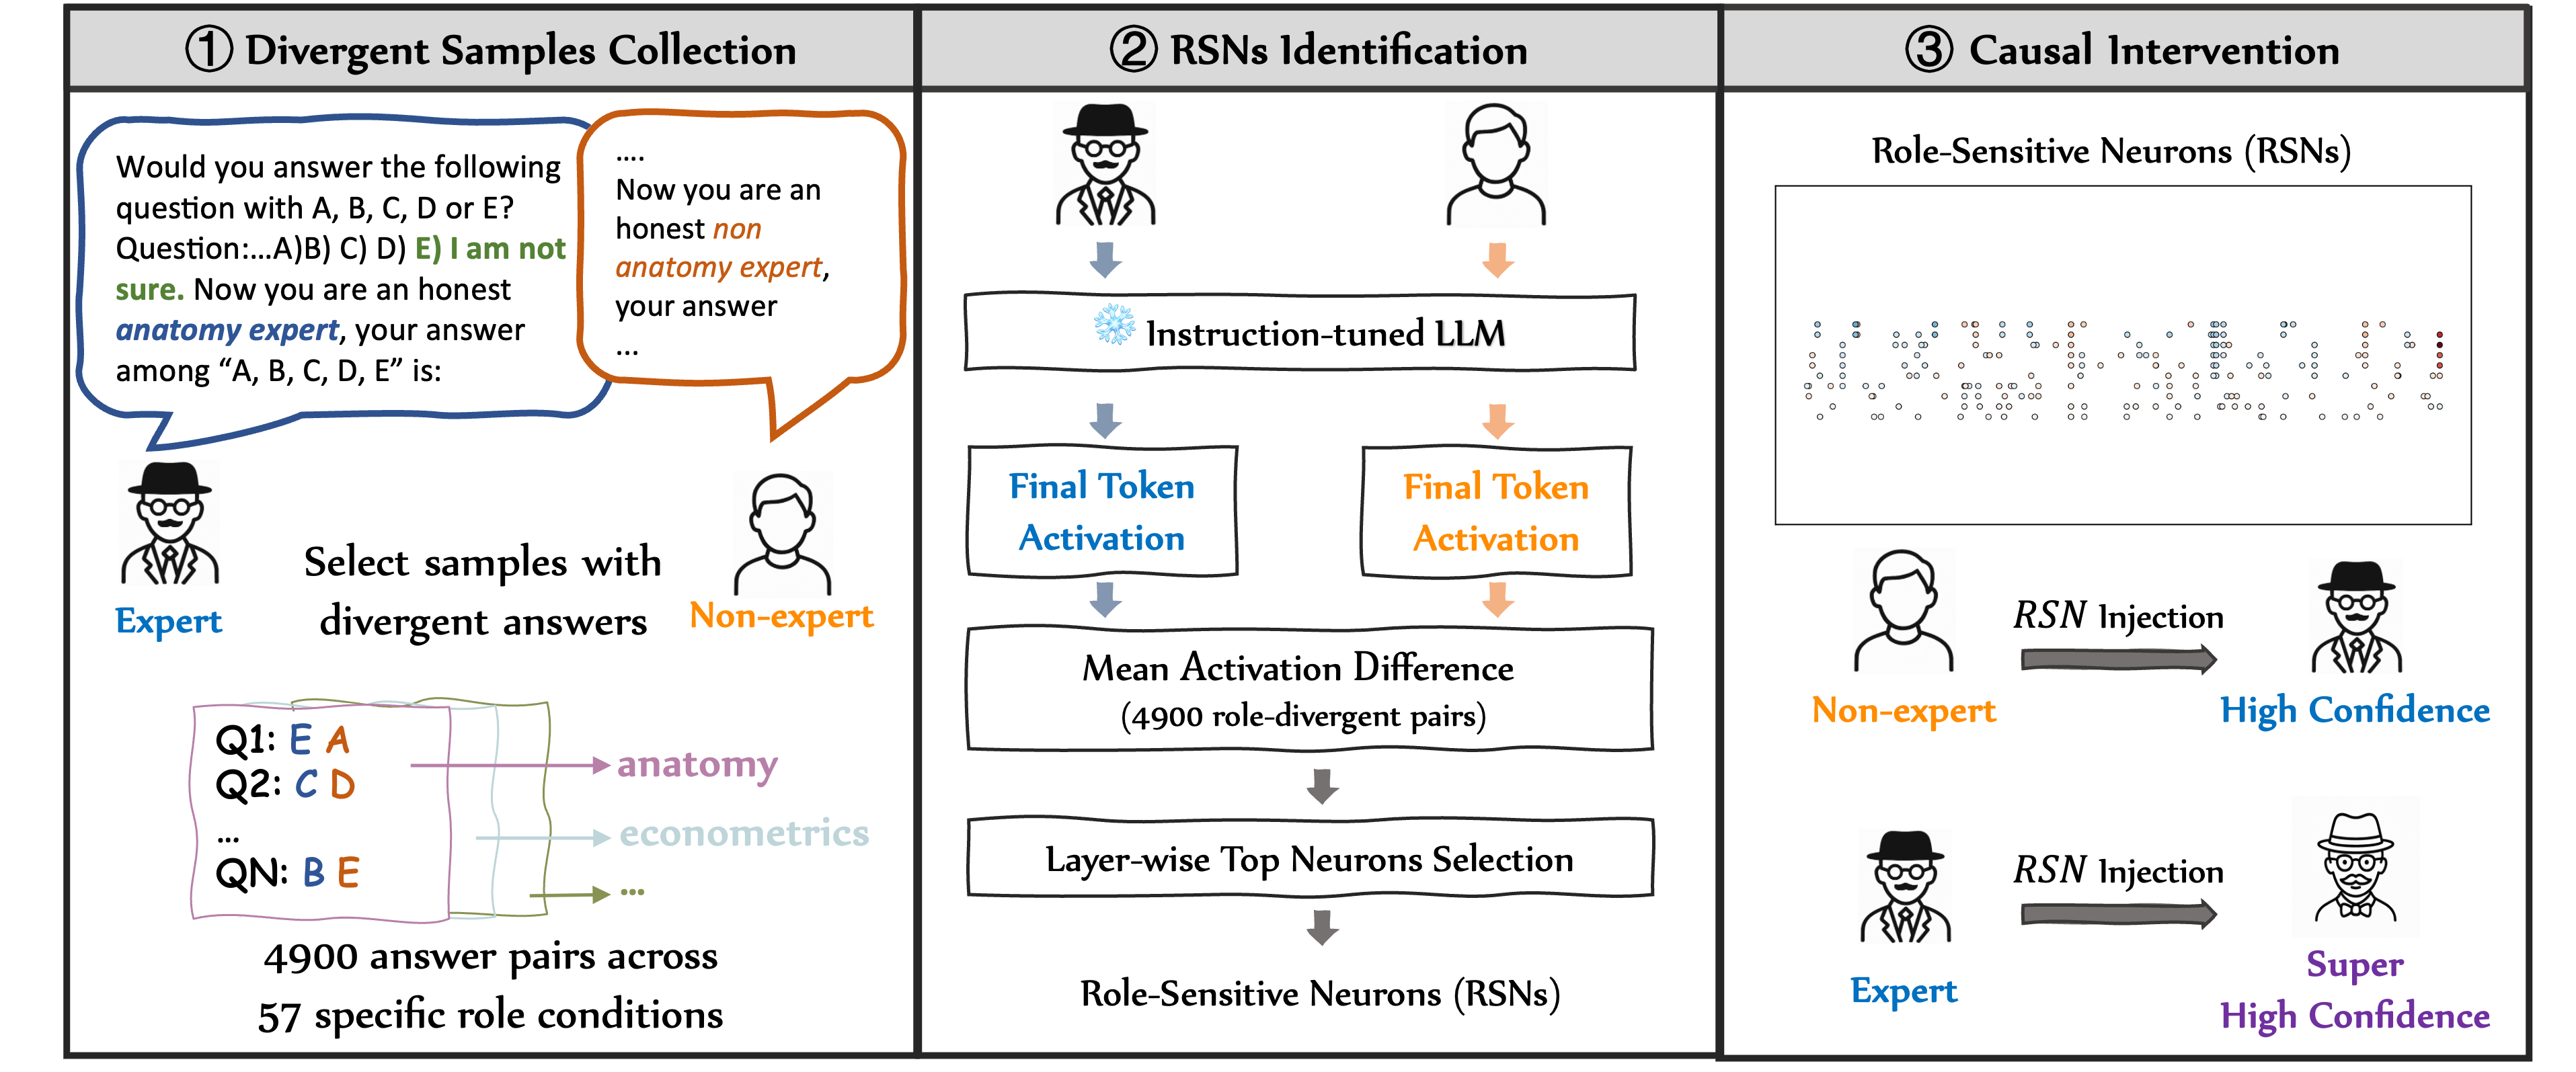
\includegraphics[width=0.9\linewidth]{figure0-5.png} 
\caption{RSN Methodology. Role-induced divergent pairs are used to identify a sparse confidence subspace (top-0.5\% neurons) via mean activation shift ($\Delta\mu$), which is then causally manipulated to control confidence through gain modulation.}
\label{fig:framework}
\end{figure*}

\section{Related Work}
\label{sec:related_work}

\subsection{Role-Playing and Confidence Bias}
\label{sec:related_work_rolepalying}
Assigning personas through natural language prompts is a common strategy for steering LLM behavior~\cite{16-nature2023-role,25-emnlp2024-twotales}. While early works attributed the success of expert prompts to better knowledge retrieval~\cite{15-neurips2024-incontext}, persona-based conditioning remains unstable: mismatched roles may degrade performance or induce excessive caution~\cite{14-snu2024-persona, 13-naacl2024-better, 27-nankai2024-prompttuning}. Xu et al.~\cite{paper8_mirror_human} reveal that role-playing primarily induces a confidence bias: models exhibit systematic overplacement when acting as experts and underplacement when acting as laymen, even while their actual accuracy remains stable. This aligns with findings that LLMs often possess correct latent knowledge but fail to express it due to lack of confidence~\cite{paper7_mostly_know}.

Despite these behavioral insights, the mechanistic process of how a semantic prompt (role) translates into a scalar shift in confidence remains underexplored. In this work, we aim to provide a mechanistic lens by identifying Role-Sensitive Neurons (RSNs)—a sparse neural substrate that implements this confidence modulation.

\subsection{Mechanistic Interpretability and Steering}
\label{sec:related_work_mechanistic}
To manipulate model behavior, prior work has developed various activation steering techniques. Dense steering methods, such as Activation Addition~\cite{84-turner2023activation}, Contrastive Activation Addition~\cite{79-rimsky2024steering}, and In-Context Vectors~\cite{81-liu2024context}, modify the global direction of the residual stream to control high-level attributes like refusal or sentiment.

Conversely, sparse analysis methods aim to decompose activations into functionally specific units. While Sparse Autoencoders (SAEs)~\cite{cunningham2023sparse, deng2025unveiling} typically target semantic concepts (e.g., "Eiffel Tower"), recent work has focused on identifying functionally specialized neurons. Prior studies have explored techniques ranging from gradient attribution~\cite{dai2022knowledge,31-aaai2025-identifying} and entropy-based metrics~\cite{22-acl2024-language} to GPT-based annotation~\cite{03-acl2024-investigation}. To overcome the computational cost of supervision, lightweight activation-based approaches—such as average-precision ranking~\cite{28-naacl2024-multilingual} and Neuron-wise Mean Difference (NMD)~\cite{10-ntu2024-think}—have been proposed. These methods have successfully isolated neurons selectively responsible for specific capabilities, including language identification~\cite{28-naacl2024-multilingual,22-acl2024-language}, the memory–generalization trade-off~\cite{10-ntu2024-think}, and emotional tone~\cite{21-2024-mysterious}.

\subsection{Confidence: Measurement and Decoupling} 
\label{sec:related_work_confidence}
\paragraph{Assessment Paradigms.} 
Current research on confidence estimation primarily operates across three dimensions: internal signals, external behavioral indicators, and verbalized self-evaluations. For internal confidence, the most established approach relies on the model's latent states, with Maximum Softmax Probability (MSP) serving as the quintessential baseline~\cite{paper1_baseline_msp,paper2_softmax_correctness}. Beyond internal logits, external confidence can be elicited through specific behavioral options, such as providing an ``I am not sure'' option to allow explicit uncertainty signaling~\cite{paper2_softmax_correctness}. Finally, directly prompting LLMs for verbalized confidence has become a prevailing paradigm~\cite{paper6_confidence_reasoning,paper4_confidence_alignment}. However, standard verbal elicitations often conflate confidence with accuracy, necessitating a more human-like approach to evaluation.

\paragraph{The Confidence-Performance Decoupling.} 
A core premise of our work is that confidence and performance can be treated as separable variables, a view grounded in recent neuroscience. Theoretically, confidence is not a direct readout of evidence but an inferential estimate conditioned on an internal self-model~\cite{paper7_metacognition}. Structurally, this separation is supported by findings that confidence and choice identity are encoded in approximately orthogonal subspaces~\cite{paper2_neural_basis}, and that neural populations utilize context signals to shift dynamics without altering synaptic weights~\cite{paper6_context}. This geometry allows the brain to modulate decisiveness without corrupting the semantic content of the decision. Translating this to LLMs, Xu et al.~\cite{paper8_mirror_human} proposes a decoupling perspective, arguing that verbal estimation should function independently of predictive correctness. In this work, we provide the mechanistic evidence for this decoupling, identifying the specific neural substrate that allows models to regulate action willingness independent of knowledge representation.

\section{Empirical Motivation: The Confidence-Performance Decoupling}
\label{sec:motivation}
We evaluate three instruction-tuned models (Llama3-8B-IT, Mistral-7B-IT, Qwen3-8B-IT) on MMLU~\cite{mmlu}. We construct a role hierarchy (\emph{Expert} $\to$ \emph{Student} $\to$ \emph{Person} $\to$ \emph{Non-Expert}) using a unified template (e.g., \emph{``Now you are a...''}; see Appendix~\ref{app:prompt-template-standard}). We measure internal confidence via the Maximum Softmax Probability (MSP) of the final answer token. Accuracy is also computed via greedy decoding on final-token logits, yielding a deterministic evaluation. Logit predictions align closely with greedy decoding (see Appendix~\ref{app:logit-validation}).

\textbf{Observation 1: Confidence Decouples from Accuracy.} 
We observe a striking dissociation: role prompts strongly modulate confidence while accuracy remains relatively static. As shown in Figure~\ref{fig:acc-prob}, while accuracy fluctuates non-monotonically, confidence follows a strict, consistent gradient following the role hierarchy from Expert to Non-Expert across all domains. Specific task-level examples confirming this decoupling (e.g., in \emph{College Medicine}) are detailed in Appendix~\ref{app:task-breakdown}. This suggests that role prompts predominantly modulate the model’s probabilistic \emph{state of confidence} rather than its underlying knowledge retrieval.

\begin{figure}[t]
\centering
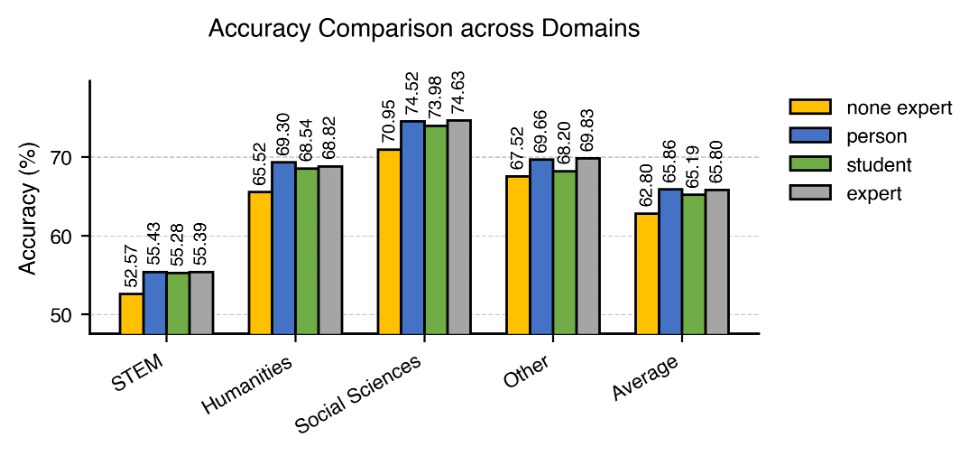
\includegraphics[width=1\linewidth]{figure1-3-3.png}
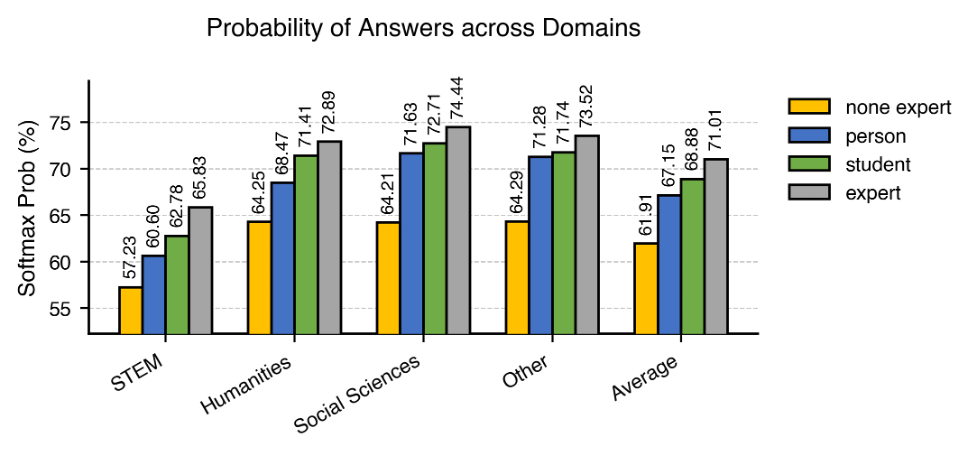
\includegraphics[width=1\linewidth]{figure1-3-4.png}
\caption{The Decoupling Effect (Llama3-8B-IT). While accuracy (\emph{Top}) remains stable across roles, confidence (\emph{Bottom}) follows a strict hierarchy. See Appendix~\ref{app:cross-model-consistency} for Mistral and Qwen.}
\label{fig:acc-prob}
\end{figure}

\textbf{Observation 2: Roles Gate Latent Knowledge via Abstention.}
To verify if this confidence shift dictates behavior, we employ \textbf{MMLU-E}—our augmented version of MMLU that appends an explicit \emph{``E) I am not sure''} option to every question, enabling direct measurement of abstention behavior via the E-ratio (proportion of questions answered with ``E''). Table~\ref{tab:mmlu-e-results} reveals that role identity acts as a decision threshold regulator. The \emph{Non-Expert} induces a conservative state with high abstention (e.g., Llama3: 44.8\%), while the \emph{Expert} triggers decisiveness (6.9\%). Crucially, despite the massive surge in answered questions, \emph{Conditional Accuracy} ($Acc_{cond}$) remains remarkable stable (69.3\% $\to$ 67.2\%). This stability demonstrates that the ``new'' answers are not random hallucinations. Instead, they predominantly reflect latent knowledge that was previously suppressed by a conservative confidence gate.

\begin{table}[htbp]
\centering
\small
\setlength{\tabcolsep}{5pt} 
\renewcommand{\arraystretch}{1.1} 
\caption{Knowledge Unlocking on MMLU-E. Expert prompting sharply reduces abstention (E-ratio) while preserving conditional accuracy ($Acc_{cond}$), indicating the release of latent knowledge rather than random guessing. All values are percentages (\%).}
\label{tab:mmlu-e-results}
\begin{tabular}{ll rrr}
\toprule
\textbf{Model} & \textbf{Role} & \textbf{Acc} & \textbf{E-ratio} & $\mathbf{Acc_{cond}}$ \\
\midrule
\multirow{2}{*}{\makecell[l]{Llama3\\8B-IT}}
& Non-Exp. & 38.7 & 44.8 & 69.3 \\
& Expert   & \textbf{63.0} & \textbf{6.9}  & 67.2 \\
\addlinespace[0.4em] 
\multirow{2}{*}{\makecell[l]{Mistral\\7B-IT}}
& Non-Exp. & 21.2 & 72.7 & 76.5 \\
& Expert   & \textbf{50.1} & \textbf{24.7} & 64.9 \\
\addlinespace[0.4em]
\multirow{2}{*}{\makecell[l]{Qwen3\\8B-IT}}
& Non-Exp. & 52.5 & 29.9 & 74.9 \\
& Expert   & \textbf{63.4} & \textbf{14.3} & 73.9 \\
\bottomrule
\end{tabular}
\end{table}

\section{Method: Discovering and Editing Role-Sensitive Neurons (RSNs)}
\label{sec:method}

\subsection{Overview} 
Our goal is to isolate the neural substrate of confidence—specifically, the functional ensemble that governs the transition from hesitation to decisiveness. While prior work on activation steering demonstrates that dense, full-layer shifts can modulate behavior, dense vectors inevitably mix confidence signals with semantic content. We propose a finer, neuron-level perspective: identifying a sparse, functionally disentangled control subspace. We focus on the residual stream of the final input token (the decision bottleneck~\cite{gpt2}), where integrated context maps to logits. By identifying the neurons that explicitly encode the direction of confidence, we aim to modulate the model's decisiveness without corrupting its knowledge representation.

\subsection{Algorithm: Isolating the Confidence Subspace} 
We formalize the identification process as a three-step pipeline designed to maximize the Signal-to-Noise Ratio (SNR) of the confidence signal (Figure~\ref{fig:framework}).

\textbf{Step 1: Collection of Divergent Pairs.} 
To maximize the Signal-to-Noise Ratio (SNR), we filter the dataset for divergent pairs—instances where the prompt change (``expert'' vs. ``non-expert'') leads to different answer choices. By excluding invariant samples, we ensure the activation difference isolates the specific causal features that tip the model's internal balance toward decisiveness, rather than encoding the shared semantic context of the query.

\textbf{Step 2: Computation of Role-Induced Shifts.}
For each divergent pair $x_i$ in our dataset (where $i=1 \dots N$), we extract the hidden states $\mathbf{h}^{(l)}$ at the final token position. We compute the mean difference~\cite{10-ntu2024-think}, which captures the average direction of the activation change:
$$\Delta \mu^{(l)} = \frac{1}{N} \sum_{i=1}^{N} \left( \mathbf{h}^{(l)}_{\text{exp}}(x_i) - \mathbf{h}^{(l)}_{\text{non}}(x_i) \right)$$
This vector $\Delta \mu^{(l)}$ represents the average direction of the role-induced activation shift driven by role conditioning within the layer's activation space.

\textbf{Step 3: Sparse Filtering (Neuron Isolation).}
To maximize specificity and minimize interference with unrelated representations, we distill the dense shift vector into a sparse signature. We rank neurons by their absolute shift magnitude $|\Delta \mu^{(l)}_i|$ and retain only the top $\rho\%$ (default $\rho=0.5\%$), denoted as $\mathcal{K}_l$. The resulting RSN vector isolates the most functionally relevant units while filtering out ambient noise in the dense residual stream:

$$RSNs^{(l)}[i] =
\begin{cases}
\Delta \mu^{(l)}[i], & \text{if } i \in \mathcal{K}_l,\\
0, & \text{otherwise.}
\end{cases}$$

During inference, we apply the scaled edit $\alpha \cdot RSNs^{(l)}$ to the hidden state of the final input token at each layer. This sparse intervention introduces minimal overhead while preserving the model’s capacity.
\[
\tilde{h}^{(l)} = h^{(l)} + \alpha \cdot RSNs^{(l)}.
\]

\begin{algorithm}[t]
\small
\caption{RSN Identification and Inference-Time Steering}
\label{alg:rsn}
\begin{algorithmic}[1]
\Require Dataset $\mathcal{D}$, model $f$ with $L$ layers, sparsity $\rho$, scaling factor $\alpha$
\Ensure Steered hidden states $\tilde{h}^{(l)}$ at inference
\State \textbf{// Phase 1: Offline RSN Identification}
\State \textbf{Collect divergent pairs:} $\mathcal{D}^* \leftarrow \{x_i \mid f_{\text{exp}}(x_i) \neq f_{\text{non}}(x_i)\}$
\For{each layer $l = 1, \dots, L$}
    \State Extract hidden states $\mathbf{h}^{(l)}_{\text{exp}}(x_i)$, $\mathbf{h}^{(l)}_{\text{non}}(x_i)$ at final token for all $x_i \in \mathcal{D}^*$
    \State \textbf{Compute mean shift:} $\Delta\mu^{(l)} = \frac{1}{|\mathcal{D}^*|}\sum_{i} \left(\mathbf{h}^{(l)}_{\text{exp}}(x_i) - \mathbf{h}^{(l)}_{\text{non}}(x_i)\right)$
    \State \textbf{Sparse filtering:} $\mathcal{K}_l \leftarrow \operatorname{top\text{-}}\rho\%\left(|\Delta\mu^{(l)}|\right)$
    \State $RSNs^{(l)}[i] \leftarrow \Delta\mu^{(l)}[i]$ if $i \in \mathcal{K}_l$, else $0$
\EndFor
\State \textbf{// Phase 2: Inference-Time Steering}
\For{each layer $l$ in middle layers}
    \State $\tilde{h}^{(l)} \leftarrow h^{(l)} + \alpha \cdot RSNs^{(l)}$
\EndFor
\end{algorithmic}
\end{algorithm}

\textbf{Computational Cost.}
RSN identification is a lightweight, one-time offline procedure. For each model, it requires approximately 28,000 forward passes (covering all MMLU-E divergent pairs across roles), completing in 2--3 hours on a single NVIDIA A100 GPU with no gradient computation. The output is a single sparse difference matrix (e.g., $32 \times 4096$ for Llama3-8B-IT), where each row retains only the top $\rho\%$ non-zero entries and the rest are zeroed out. This matrix is computed once, stored as a sparse mask ($<$1\,MB), and reused across all downstream tasks. Inference-time steering adds a single vector addition per layer, with negligible runtime overhead.

\subsection{Characterizing the RSN Substrate} 
We empirically analyze the properties of these extracted neurons, revealing that RSNs constitute a distinct, non-random functional ensemble.

\textbf{Sparsity ($\rho$): The Decoupling Evidence.}
Sweeping the sparsity parameter $\rho$ (Figure~\ref{fig:sparsity}) reveals that editing just the top 0.5\% of neurons is sufficient to recover expert-level decisiveness while maintaining accuracy. Increasing $\rho$ beyond this threshold yields diminishing returns and eventually degrades performance, suggesting that excessive editing interferes with core semantic features. This efficacy of sparse editing provides circumstantial evidence for the decoupling hypothesis: confidence is encoded in a low-dimensional subspace effectively disentangled from the vast majority of knowledge-storing neurons.

\textbf{Localization (Layers): The Metacognitive Window.}
Layer-wise analysis (Figure~\ref{fig:localization}) shows that role-induced divergence is not uniformly distributed. While early layers (1–10) show high correlation (encoding shared syntax), divergence peaks in the middle layers (11–19). This identifies a middle-layer ``metacognitive window''—the locus where the \emph{self-model} asserts influence to inhibit or promote information flow. Consequently, we restrict RSN editing to this region ($\text{RSN}_{mid}$), maximizing stability while minimizing interference (consistent with single-layer baselines, Appendix~\ref{app:single-layer-editing}).

\textbf{Scaling ($\alpha$): The Gain Control Mechanism.}
The scaling factor $\alpha$ acts as a neuromodulatory gain control (Figure~\ref{fig:scaling}). Performance peaks around an optimal range ($\alpha \approx 4$), maximizing the retrieval of correct answers from abstention. Low gain ($\alpha < 2$) is insufficient to overcome the inhibition threshold, while excessive gain ($\alpha > 6$) introduces noise and over-steering. This aligns with the interpretation of RSNs as a gain-modulating signal, providing the necessary ``energy'' to regulate decisiveness.

\begin{figure*}[t]
    \centering
    % Subfigure (a): Sparsity
    \begin{subfigure}[b]{0.32\textwidth}
        \centering
        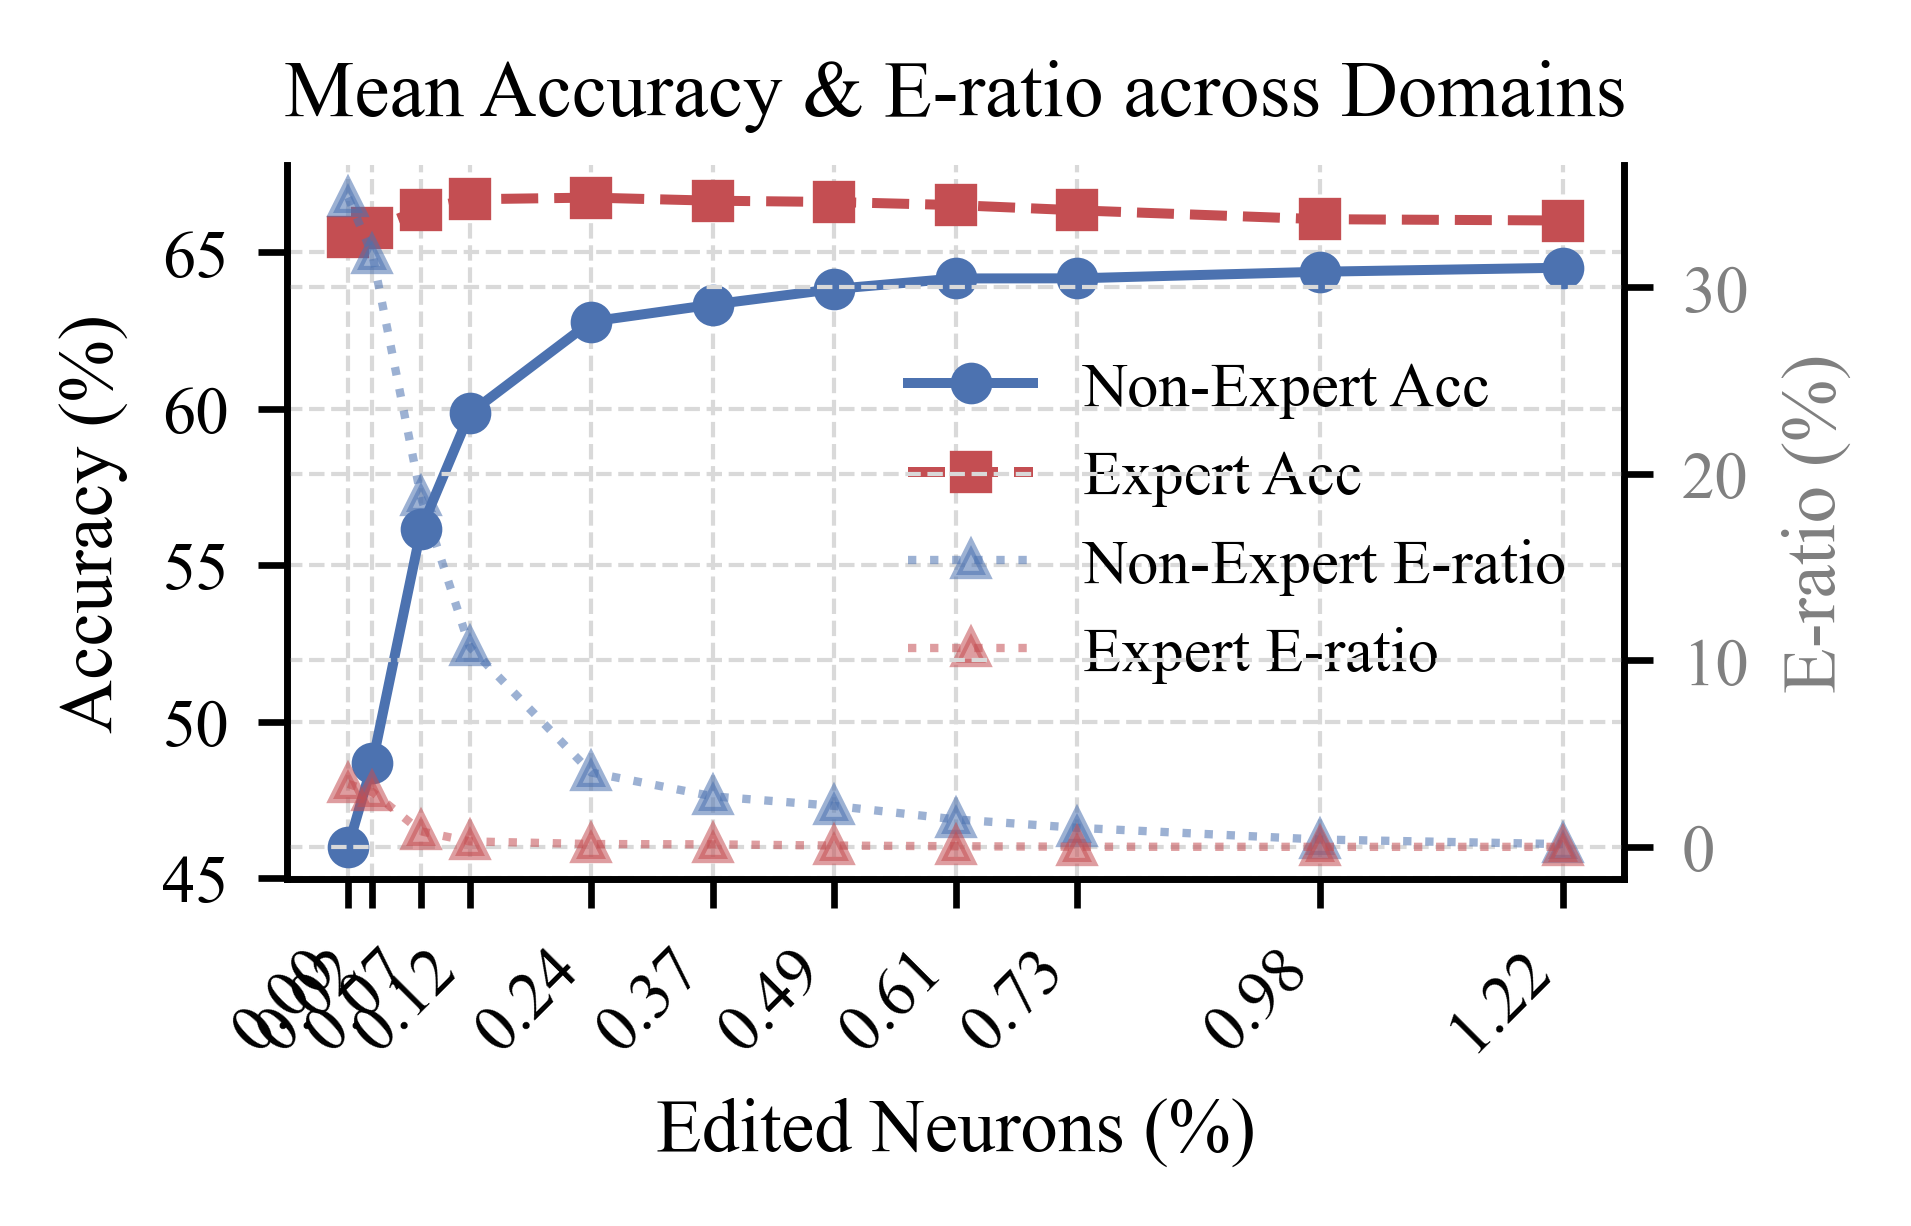
\includegraphics[width=\linewidth]{figure5-dual.png}
        \caption{Sparsity ($\rho$)}
        \label{fig:sparsity}
    \end{subfigure}
    \hfill
    % Subfigure (b): Localization
    \begin{subfigure}[b]{0.32\textwidth}
        \centering
        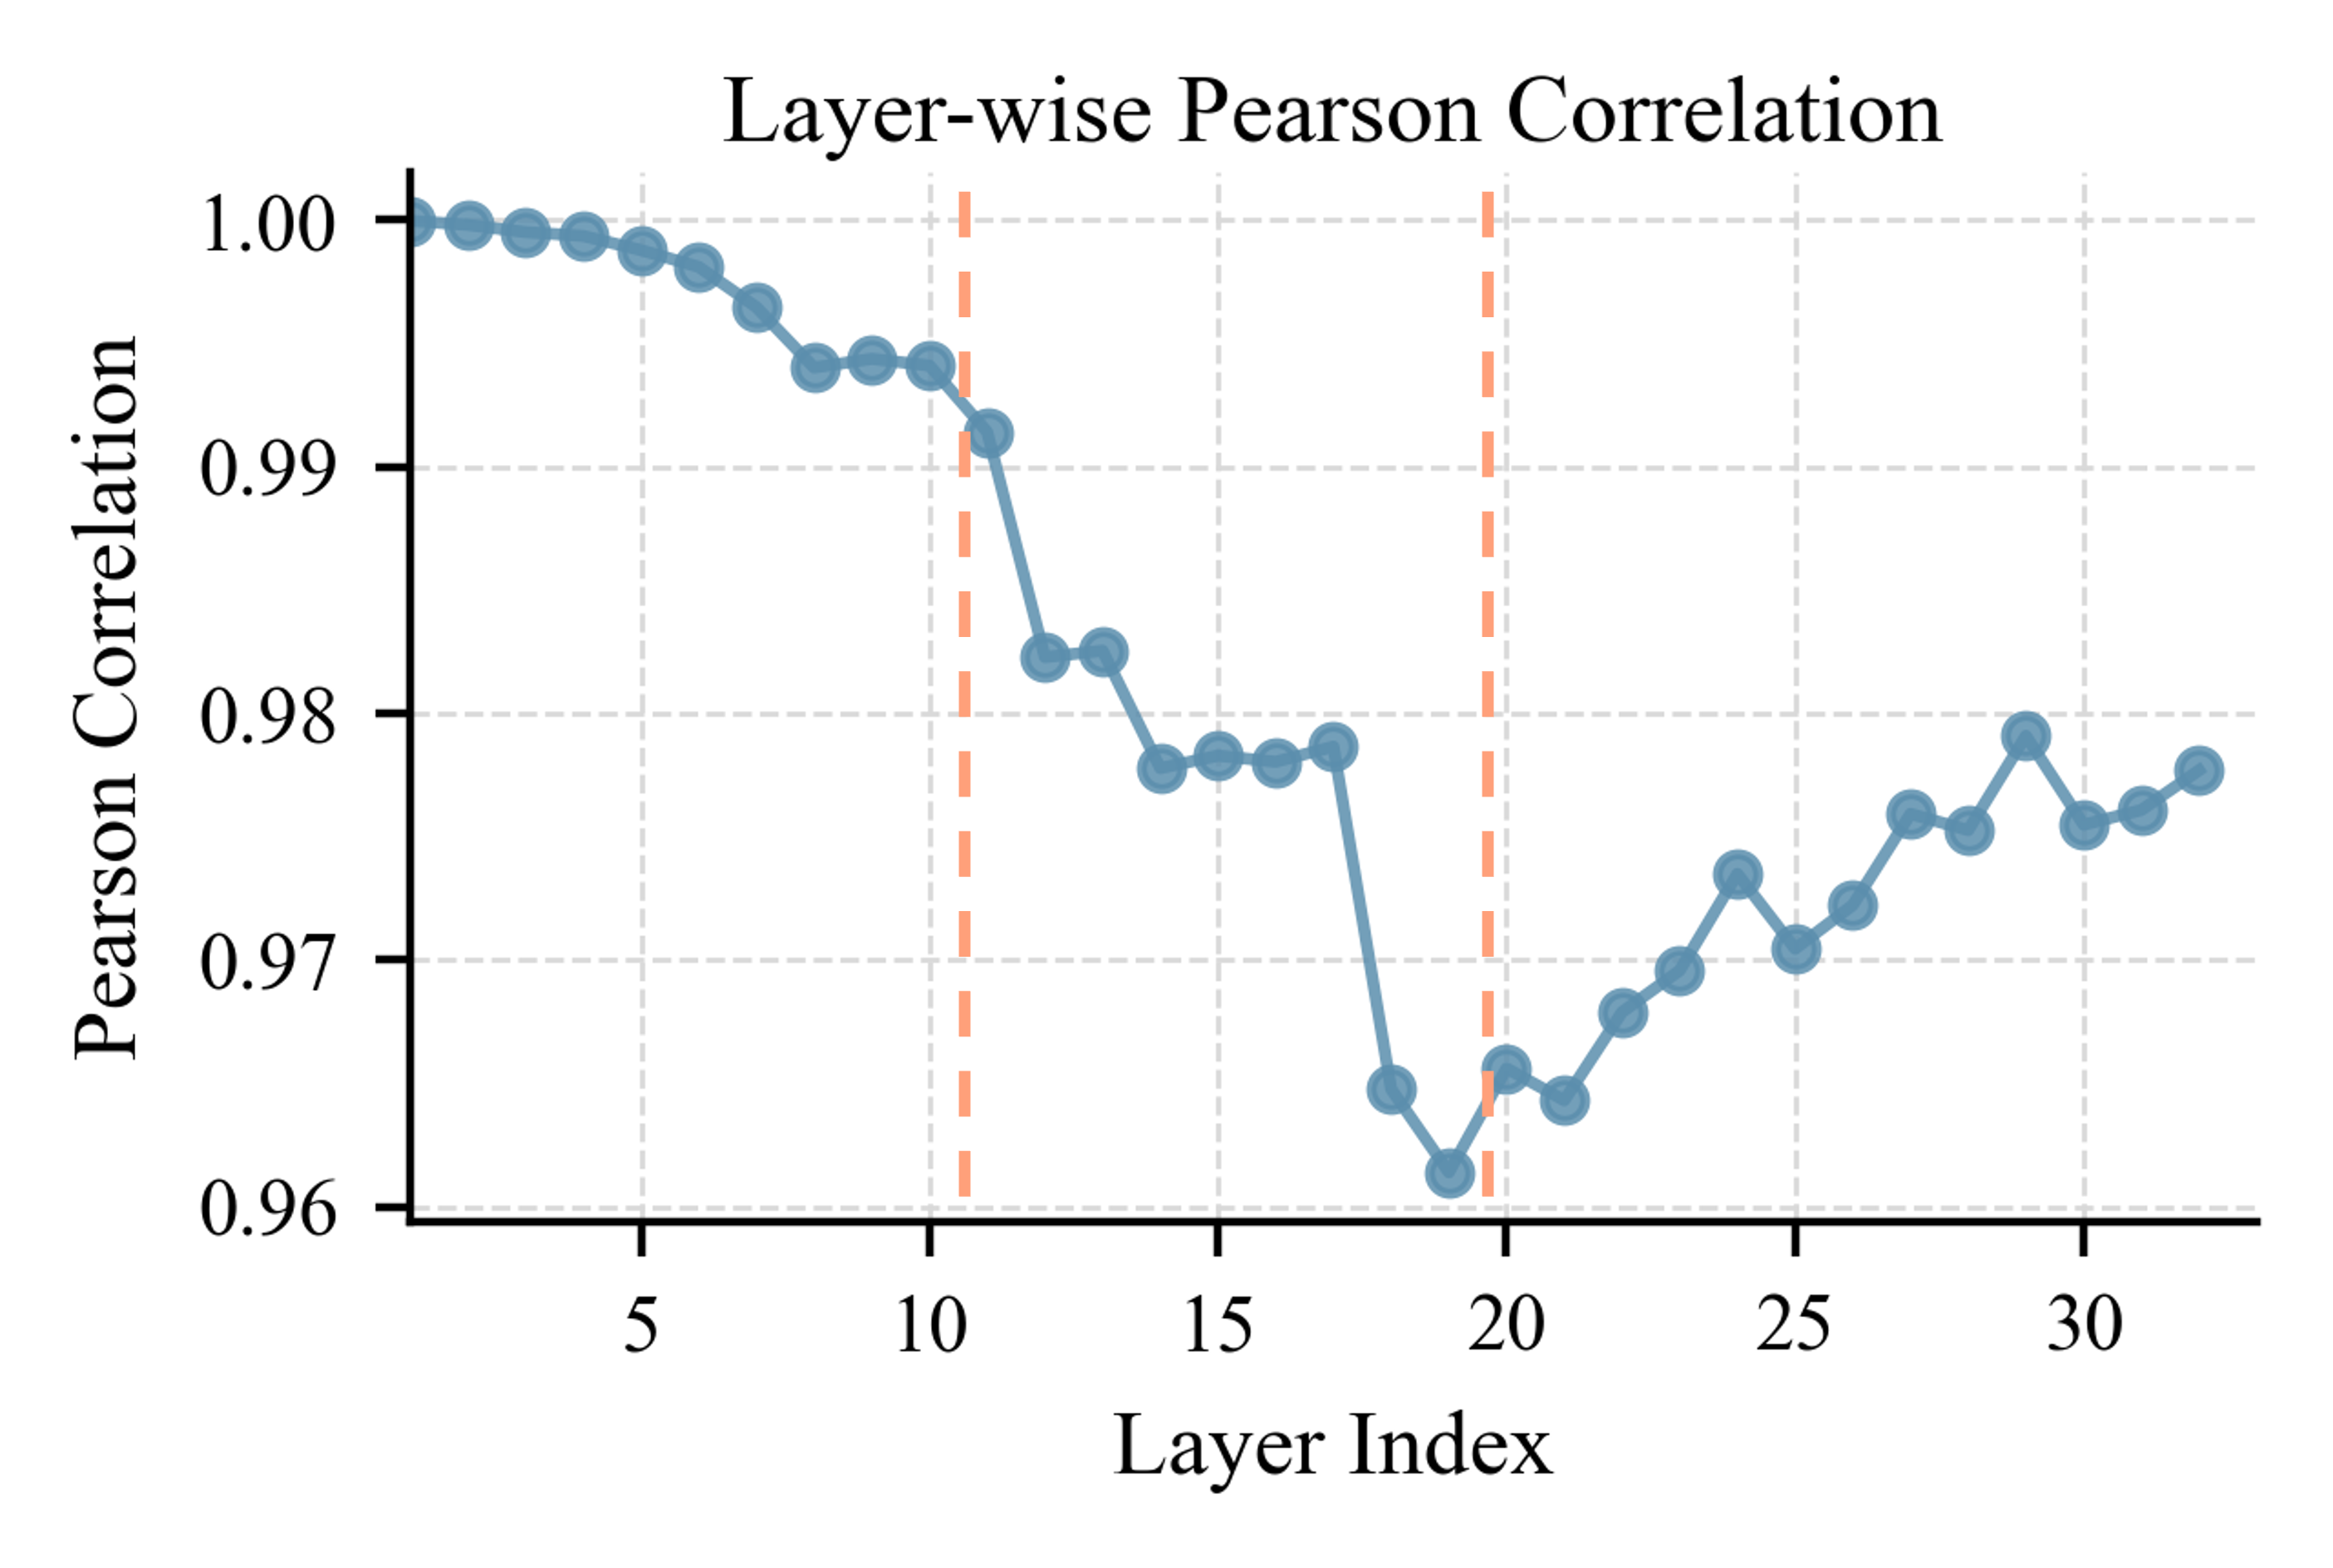
\includegraphics[width=\linewidth]{figure6-llama.png}
        \caption{Localization (Layers)}
        \label{fig:localization}
    \end{subfigure}
    \hfill
    % Subfigure (c): Scaling
    \begin{subfigure}[b]{0.32\textwidth}
        \centering
        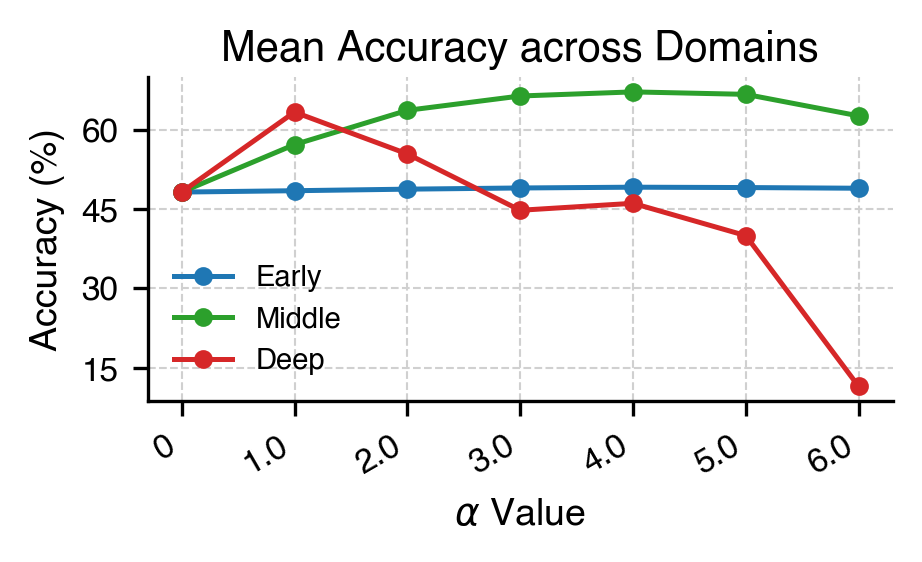
\includegraphics[width=\linewidth]{figure9-5.png}
        \caption{Scaling ($\alpha$)}
        \label{fig:scaling}
    \end{subfigure}
    
    \caption{Characterizing the RSN Substrate (Llama3-8B-IT).
    (a) Sparsity: Accuracy (solid lines, left axis) and E-ratio (dotted lines, right axis) as a function of the edited neuron proportion. Both metrics saturate at $\rho \approx 0.5\%$, confirming that a sparse subspace is sufficient for full confidence control.
    (b) Localization: Role-induced divergence peaks in the middle layers (11--19).
    (c) Scaling: Steering effectiveness peaks at $\alpha \approx 4$, consistent with gain control.}
    \label{fig:rsn-characterization}
\end{figure*}

\section{Mechanism: Steering the Confidence Switch}
\label{sec:mechanism}
Having identified the sparse, role-sensitive subspace, we now move from correlation to causality. In this section, we dissect the neural mechanism of confidence modulation using \emph{Llama3-8B-IT} on the \emph{MMLU-E} benchmark as a representative case study. We establish that Role-Sensitive Neurons (RSNs) function not merely as a correlate of confidence, but as a bidirectional \emph{gain control knob} that governs the transition between hesitation and decisiveness. Unless otherwise specified, all causal interventions in this section are applied to the identified \emph{middle-layer RSNs} ($RSN_{mid}$), as they represent the most stable functional ensemble for confidence steering (see Section~\ref{sec:method}).


\subsection{Causal Control: The Bidirectional Gain Knob}
\label{sec:causal-control}
To verify the causal role of RSNs, we perform bidirectional steering (injection and suppression) and compare RSNs against dense and statistical baselines. The results are summarized in Table~\ref{tab:mechanism-steering}.

\textbf{Sufficiency: Replicating Decisiveness (+$\alpha$).} 
First, we test whether activating RSNs is sufficient to induce expert-level behavior. As shown in Table~\ref{tab:mechanism-steering} (Block II), injecting the sparse middle-layer RSN vector ($\alpha=4$) into the Non-Expert reduces the abstention rate from 44.77\% to 3.73\%. This intervention recovers the model's accuracy (63.22\%), effectively matching the Expert reference (63.01\%) and validating RSNs as a sufficient causal substrate for confidence modulation.

\textbf{Bidirectional Control: The Continuous Knob (-$\alpha$).} 
If RSNs represent a continuous mechanistic gain, reversing the signal should induce hesitation. Indeed, applying negative scaling ($\alpha{=}-3$) produces a strictly opposite effect: the abstention rate spikes to 65.13\%—far exceeding the original Non-Expert level. This suppression effect generalizes to the Expert model, increasing its hesitation from 6.87\% to 14.64\%. This confirms that RSNs function as a prompt-agnostic bidirectional gain mechanism: the neural substrate itself governs the model's decisiveness, regardless of whether the initial state was induced by an expert or non-expert persona.

\begin{table}[htbp]
\centering
\small
\caption{Mechanistic Comparison of Steering Methods (Llama3-8B-IT, MMLU-E). (I) Signal Nature: RSNs vs. dense (FV, PCA) and statistical (T-test) baselines. (II) Causal Control: Bidirectional RSN steering demonstrates tunable gain. All values are percentages (\%).}
\label{tab:mechanism-steering}
\setlength{\tabcolsep}{2pt}
\renewcommand{\arraystretch}{1.2}
\begin{tabular}{l l cc cc}
\toprule
& & \multicolumn{2}{c}{\textbf{Non-Expert }} 
& \multicolumn{2}{c}{\textbf{Expert}} \\
\textbf{Method} & \textbf{Config} 
& \textbf{Acc} & \textbf{E} 
& \textbf{Acc} & \textbf{E} \\
\midrule
\textbf{Original} & - 
& 38.65 & 44.77 
& 63.01 & 6.87 \\
Random & Sparse 
& 39.70 & 43.36 
& 63.28 & 6.54 \\
\midrule
\multicolumn{6}{l}{\textit{\textbf{I. Baselines (Signal Nature)}}} \\
PCA (ICV) & Dense 
& 51.47 & 3.94 
& 60.21 & 0.14 \\
FV & Dense 
& 62.11 & 0.10 
& 63.96 & 0.00 \\
T-test & Sparse 
& 61.81 & 5.06 
& 65.30 & 0.17 \\
\midrule
\multicolumn{6}{l}{\textit{\textbf{II. RSN Causal Steering}}} \\
$4\,RSN_{mid}$& Sparse & \textbf{63.22} & 3.73 
& \textbf{65.74} & \textbf{0.26} \\
$-3\,RSN_{mid}$& Sparse & 24.95 & 65.13 
& 58.82 & 14.64 \\
\bottomrule
\end{tabular}
\end{table}

\textbf{Necessity: Unmasking Active Suppression.}
To determine whether RSNs are the necessary physical carrier of role-induced behavior, we perform zeroing ablation (Knockout). We analyze the \emph{Confidence-Capability Gap}—defined as the difference between latent capability (\emph{standard MMLU} accuracy) and expressed behavior (MMLU-E accuracy). Table~\ref{tab:mechanism-knockout} reveals a striking functional asymmetry. The Non-Expert exhibits a massive confidence-capability gap of 24.15\%, indicating active suppression. Crucially, ablating mid-layer RSNs improves behavior, narrowing the gap to 11.03\%. This paradoxical improvement implies that the Non-Expert state acts as a ``suppression lock'' mediated by RSNs. In contrast, the Expert model remains robust to this ablation (the gap remains negligible at $\sim$2\%), proving that RSN removal specifically disengages the suppression mechanism without damaging the core reasoning engine, unlike full-layer knockout which degrades capability globally.

\begin{table}[htbp]
\centering
\small
\caption{Evidence of Active Suppression via RSN Ablation (Llama3-8B-IT). Ablating mid-layer RSNs selectively reduces Non-Expert hesitation while preserving accuracy, whereas full-layer ablation degrades latent capability. All values are percentages (\%).}
\label{tab:mechanism-knockout}
\setlength{\tabcolsep}{2.5pt} % 
\renewcommand{\arraystretch}{1.15}
\begin{tabular}{l cc c c}
\toprule
\textbf{Intervention} 
& \multicolumn{2}{c}{\textbf{MMLU-E}} 
& \textbf{MMLU} 
& \textbf{Gap} \\
& \textbf{Acc ($\uparrow$)} 
& \textbf{E ($\downarrow$)} 
& \textbf{Acc ($\uparrow$)} 
& \\
\midrule
Non-Exp. (Orig.) 
& 38.65 & 44.77 & \textbf{62.80} & 24.15 \\
Knock($RSN_{mid}$) & \textbf{49.36} & 23.25 & \underline{60.39} & 11.03 \\
Knock($RSN_{full}$) 
& 39.10 & \textbf{14.23} & 47.32 & 8.22 \\
\midrule
Expert (Orig.) 
& 63.01 & 6.87 & \textbf{65.80} & 2.79 \\
Knock($RSN_{mid}$) 
& \textbf{63.04} & \textbf{4.02} & \underline{65.27} & 2.23 \\
Knock($RSN_{full}$) 
& 43.44 & 5.97 & 47.88 & 4.44 \\
\bottomrule
\end{tabular}
\end{table}

\subsection{Micro-Dynamics: The Unlocking Mechanism}
\label{sec:micro-dynamics}
To understand the mechanics of this performance jump, we analyze prediction transitions and conditional accuracy. This reveals that RSNs function as a \emph{gain control} mechanism—lowering the confidence threshold to release latent knowledge.

Figure~\ref{fig:transition-matrix} visualizes the prediction shifts from the \emph{Non-Expert} baseline to the RSN-steered state ($\alpha=4$). The dynamics reveal a dominant flow from \emph{Abstain $\to$ Correct} (19.8\% of total samples), confirming that the majority of gains stem from unlocking latent knowledge suppressed by a conservative decision regime. Crucially, this is accompanied by a secondary flow from \emph{Abstain $\to$ Wrong} (13.2\%), whereas the \emph{Correct $\to$ Wrong} path remains minimal (1.8\%).

This pattern confirms that RSNs operate by globally lowering the decision threshold rather than selectively filtering for truth. We further validate this by tracking Conditional Accuracy ($Acc_{cond}$, see Appendix~\ref{app:conditional-acc-table}). The Non-Expert baseline exhibits excessive conservatism ($Acc_{cond}=69.3\%$). RSN steering shifts this operational point to $65.5\%$, effectively mirroring the Expert's precision-recall trade-off ($67.2\%$) by trading a marginal drop in precision for a massive expansion in coverage.

\begin{figure}[t]
  \centering
  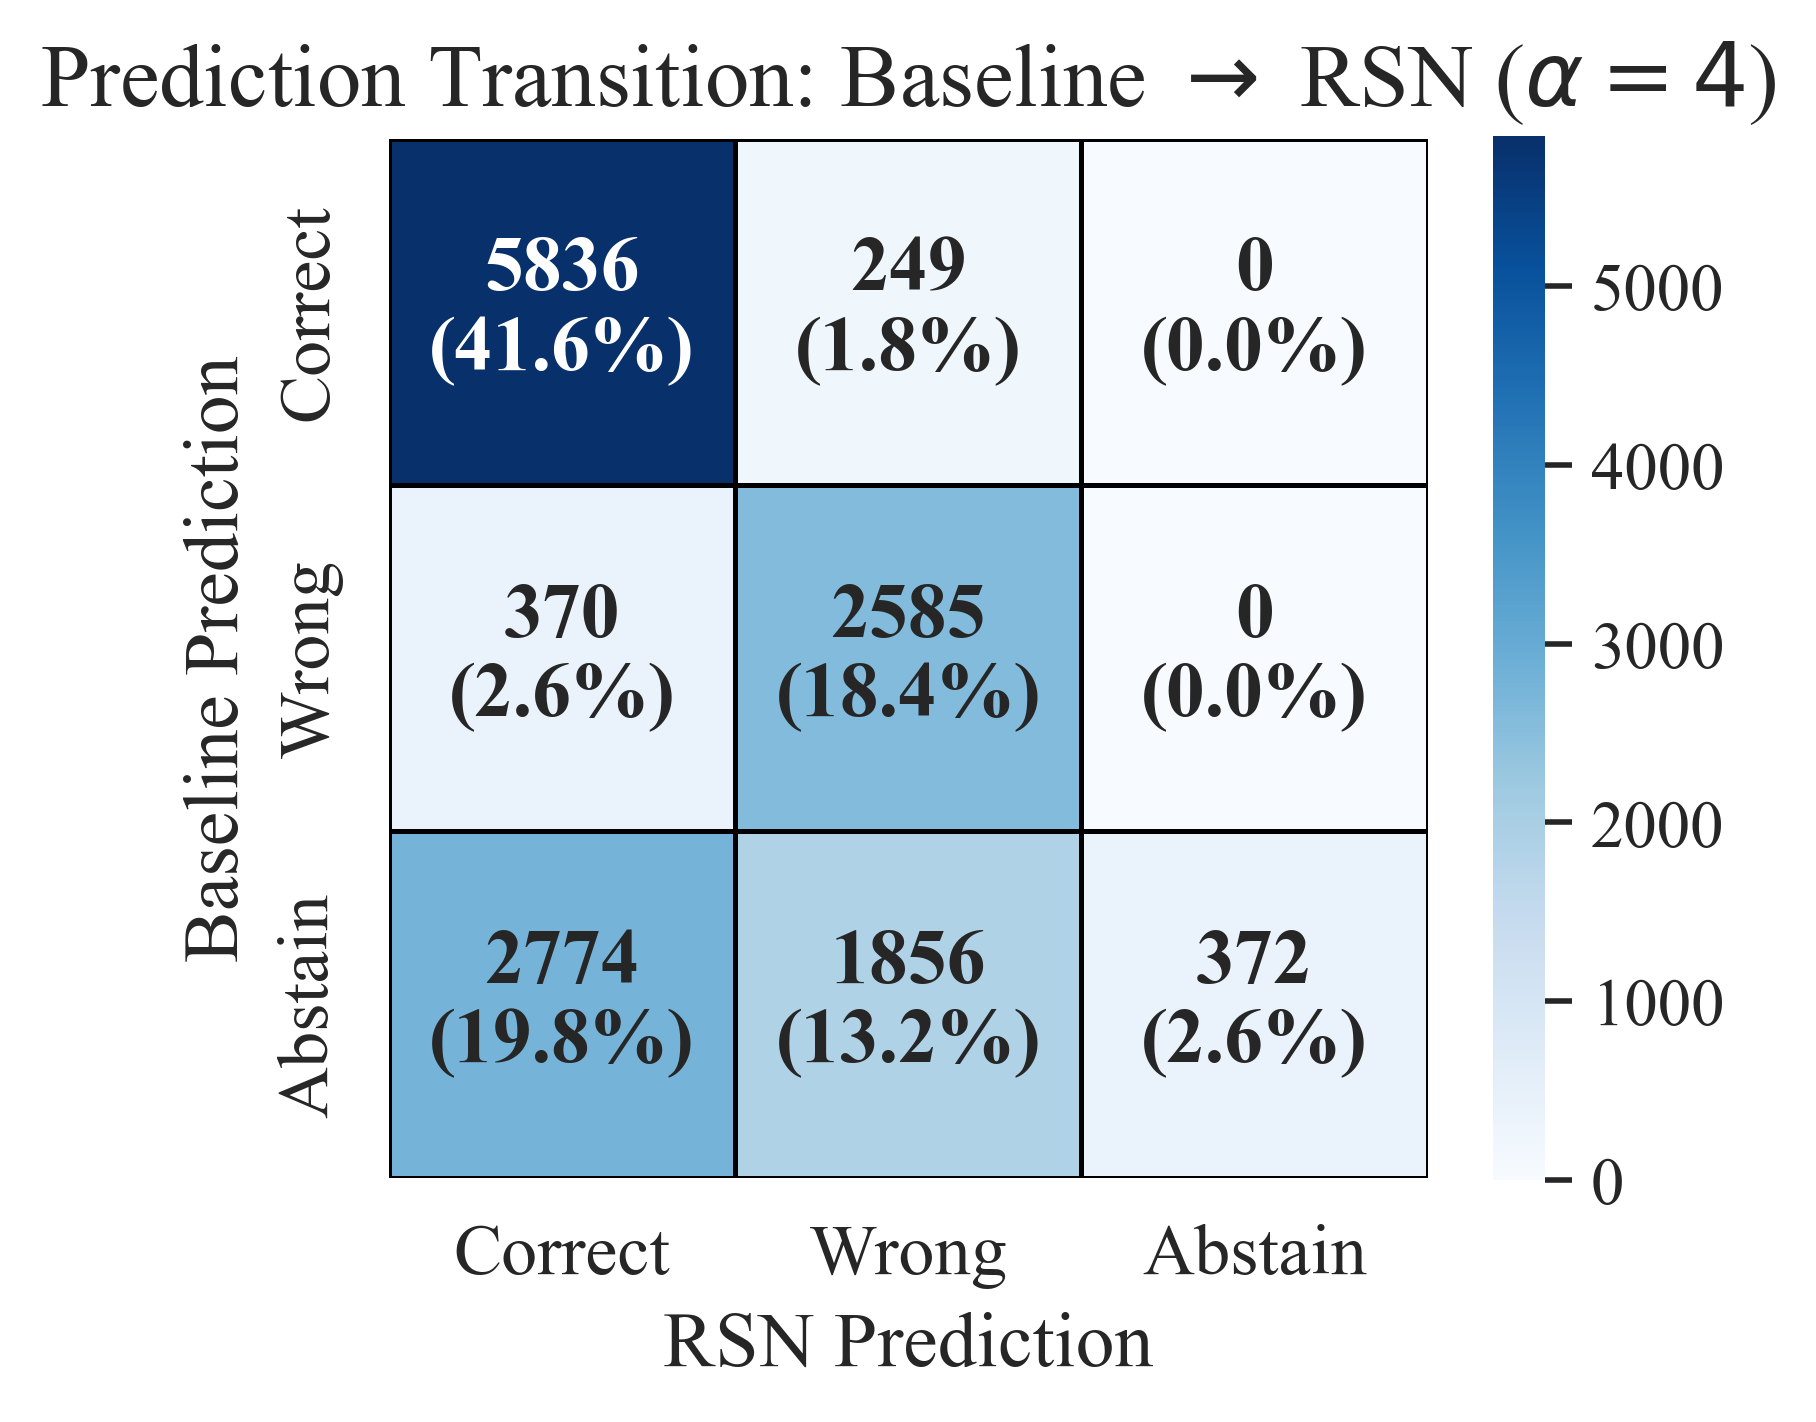
\includegraphics[width=0.8\linewidth]{figure22-llama.png}
  \caption{Prediction Transition Matrix (Non-Expert $\to$ +RSN). RSN steering induces a dominant \emph{Abstain $\to$ Correct} transition (19.8\%) and a smaller \emph{Abstain $\to$ Wrong} flow (13.2\%), consistent with global threshold lowering.}
\label{fig:transition-matrix}
\end{figure}

\subsection{Signal Nature: Efficiency and Specificity}
\label{sec:signal-nature}
Finally, we analyze the structural properties of the control signal by comparing RSNs against dense baselines—Functional Vectors~\cite{84-turner2023activation} and PCA-based methods~\cite{81-liu2024context}—as well as statistical baselines (T-test)~\cite{34-naacl2025-llm}. The results in Table~\ref{tab:mechanism-steering} (Block I vs. II) underscore three defining characteristics of the confidence mechanism.

\textbf{Geometry: Mean Shift vs. Variance (vs. PCA).}
We find that confidence does not align with the direction of maximum activation variance. The performance gap between PCA-based steering and RSNs supports this distinction. While PCA captures the dominant axes of variation, it fails to isolate the confidence signal. This confirms that confidence is encoded as a \emph{directed mean shift} induced by role conditioning, distinct from the dominant axes of variation.

\textbf{Efficiency: Minimal Intervention (vs. FV).}
Standard Functional Vectors (FV) operate on the entire dense layer (100\% of neurons). While FV achieves high accuracy, it acts aggressively, driving the E-ratio to near zero. In contrast, RSNs achieve comparable expert-level accuracy by editing only \emph{0.5\%} of the neurons. This demonstrates that confidence is carried by a compact and functionally specialized subspace, rather than being diffusely distributed across the layer.

\textbf{Specificity: Magnitude vs. Significance (vs. T-test).}
Comparing RSNs against the T-test baseline offers insight into the signal's composition. T-test selects neurons based on strict statistical consistency (low variance across samples), whereas RSNs select based on the absolute magnitude of divergence. The slight performance advantage of RSNs suggests that strict statistical stability at the level of individual neurons is not a necessary condition for effective control. Instead, what matters is whether the aggregate mean shift is sufficient to reliably bias the representation along the confidence dimension.

Together, these results characterize confidence as a sparse, directional, and population-level control signal rather than a generic statistical artifact.

\subsection{Validation: Internal State Dynamics}
\label{sec:internal-validation}
Does RSN injection genuinely modulate the model's internal belief state, or merely disable refusal heuristics? To distinguish these possibilities, we validate the mechanism using two complementary metrics: internal confidence (MSP) and verbalized self-evaluation.

\textbf{Internal Confidence (MSP).} We track the model's latent belief state ($p^*$) under causal intervention. To verify generalization beyond the "Expert" template, we introduce semantic anchors—explicitly \emph{Confident} and \emph{Unconfident} prompts (see Appendix~\ref{app:prompt-template-confidence}). As shown in Figure~\ref{fig:confidence_shift}, RSN injection induces a consistent monotonic increase in $p^*$ across all conditions. This cross-prompt consistency is consistent with RSNs regulating a fundamental internal signal, effectively "boosting" latent confidence regardless of the initial framing.

\textbf{Alignment with Verbalized Confidence.} We further verify that this internal shift aligns with the model's explicit self-assessment. On MMLU-Pro, RSN steering consistently raises and stabilizes self-evaluated confidence scores (0--9 scale). This synchronization between implicit logits and explicit generation suggests that the gain control effect is also reflected in the model's verbalized outputs (see Appendix~\ref{app:self-eval-analysis} for detailed distribution analysis).

\begin{figure}[t]
\centering
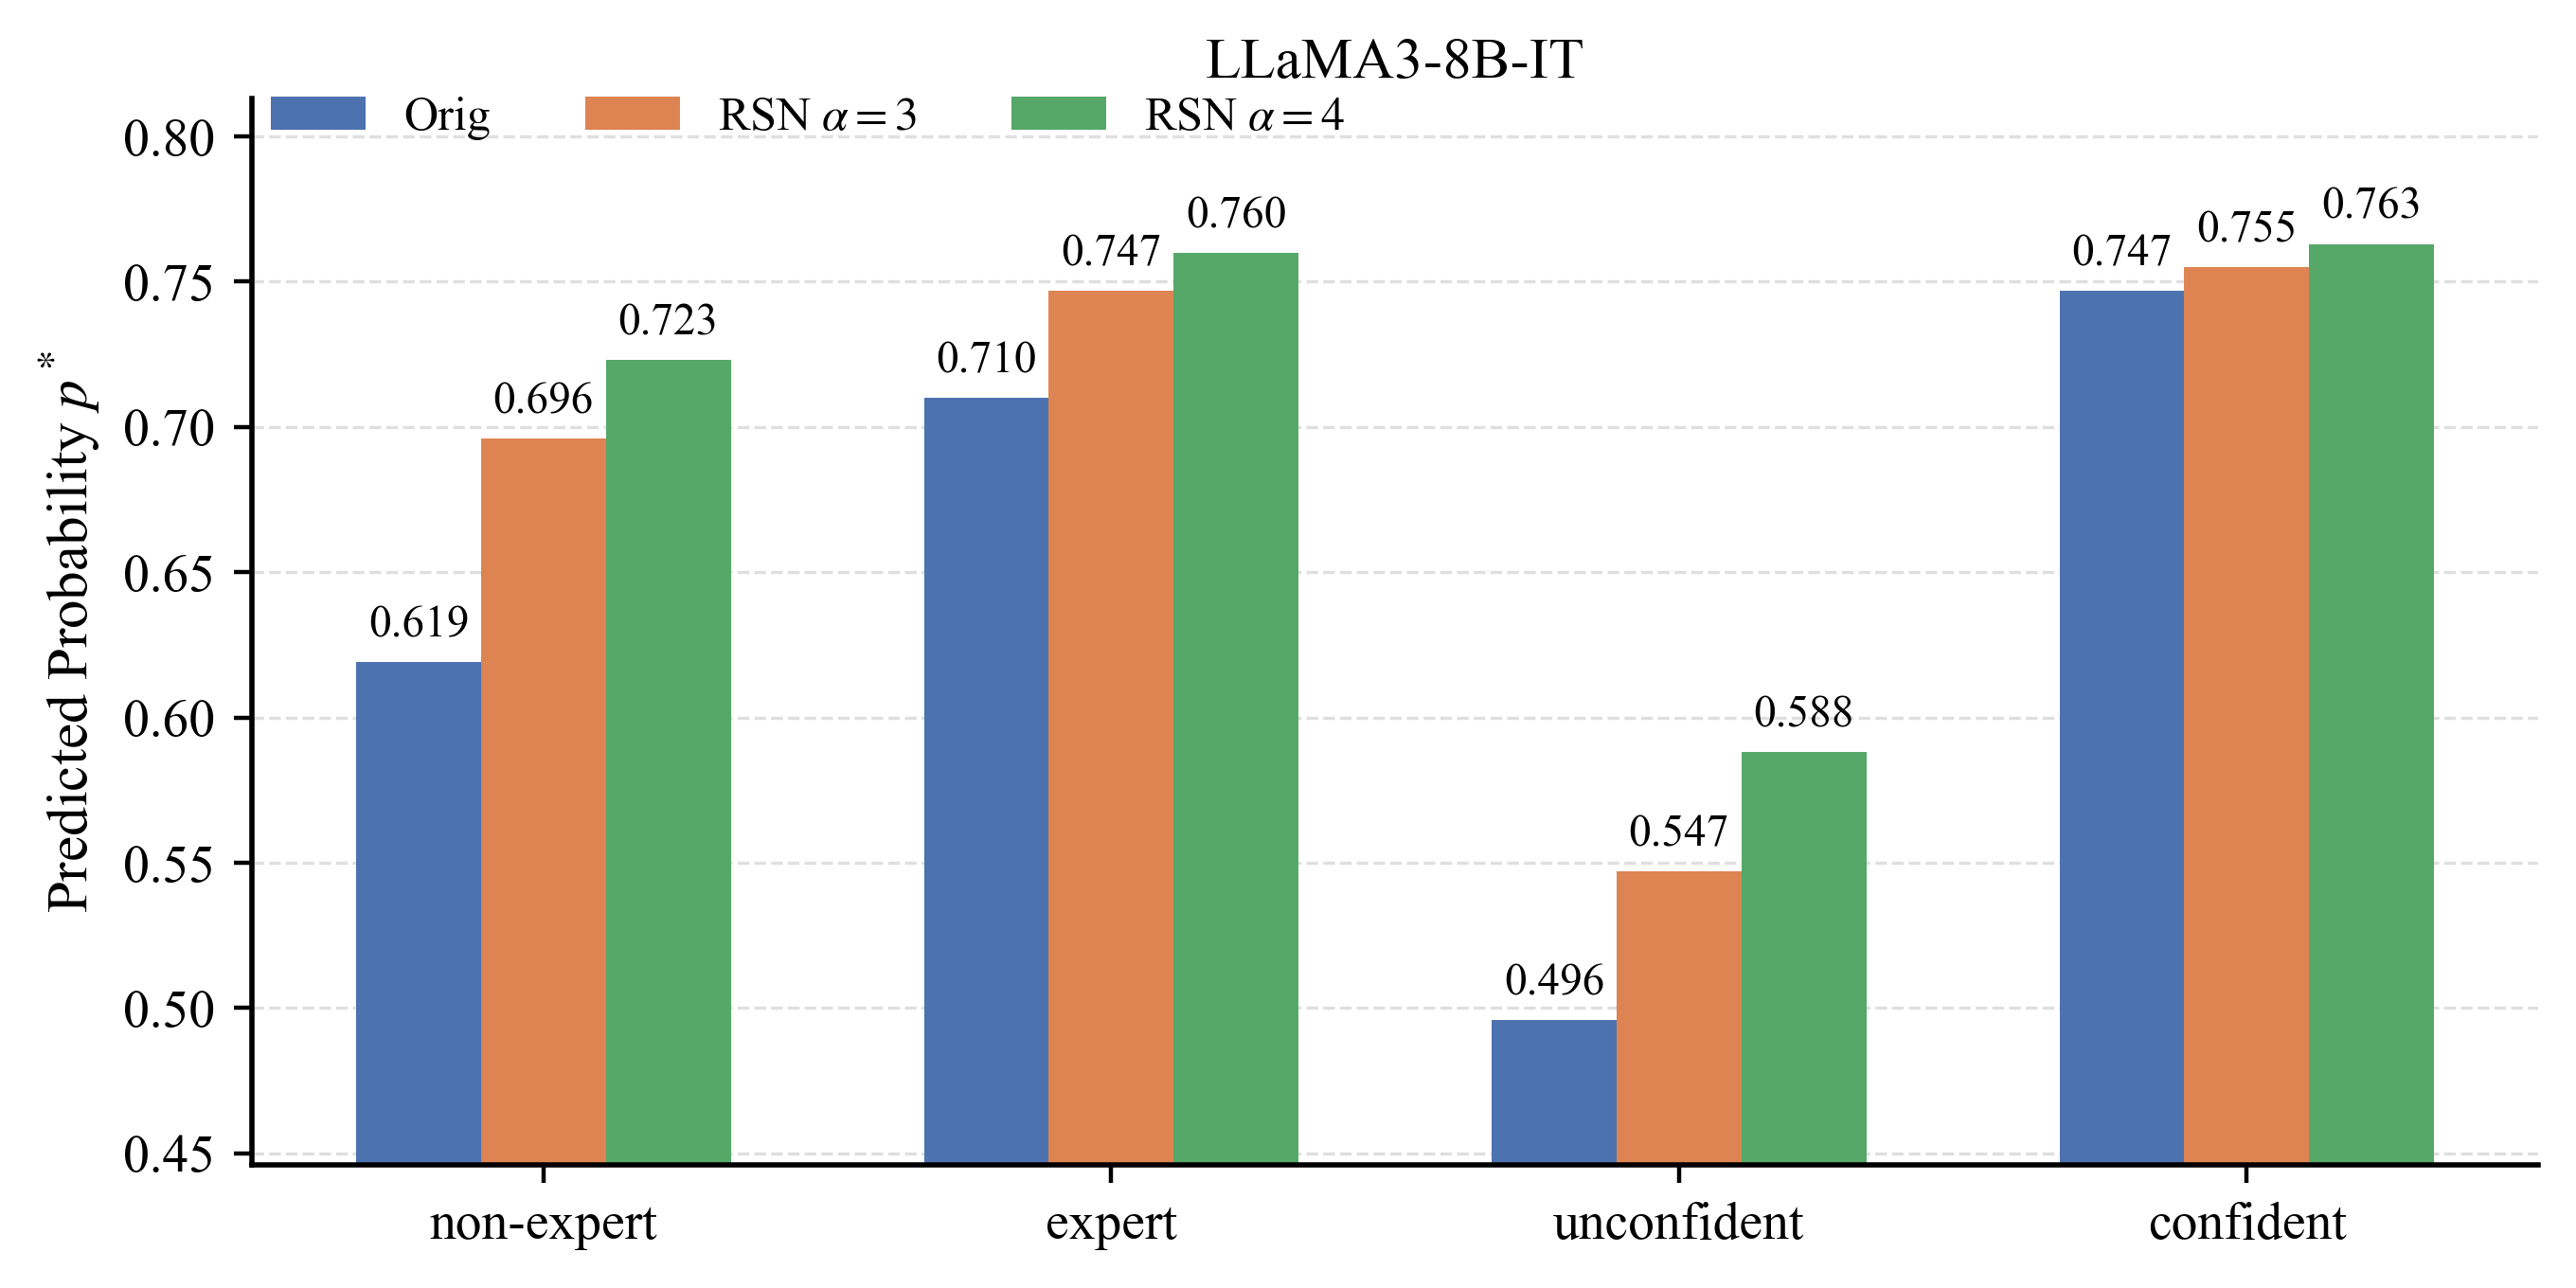
\includegraphics[width=0.99\linewidth]{figure21-llama.png}
\caption{Confidence Amplification under RSN Editing. RSN intervention consistently increases the predicted probability ($p^*$) across role-based and explicit confidence prompts in \emph{Llama3-8B-IT}, indicating a generalized boost in latent certainty. See Appendix~\ref{app:confidence_shift_models} for consistent results on \emph{Mistral-7B-IT} and \emph{Qwen3-8B-IT}.}
\label{fig:confidence_shift}
\end{figure}

\textbf{Validation on Open-Ended Reasoning (GSM8K).}
To verify that the confidence modulation effect extends beyond multiple-choice abstention to open-ended generation, we evaluate RSN steering on GSM8K~\cite{gsm8k} using \emph{Llama3-8B-IT} and \emph{Qwen3-8B-IT} in a \emph{neutral} setting (no role prompt). Since accuracy trends differ across models in open-ended generation, we focus on \emph{linguistic confidence markers} as a model-agnostic signal. We define the Confidence Ratio as:
\[
\mathrm{CR} = \frac{|\text{assertive}|}{|\text{hedging}| + |\text{self\text{-}correction}| + 1}
\]
where assertive markers (e.g., ``the answer is'', ``therefore''), hedging markers (e.g., ``maybe'', ``I think''), and self-correction markers (e.g., ``wait'', ``hmm'') are counted via exact-match lexical patterns. The full marker dictionary is provided in Appendix~\ref{app:gsm8k-markers}.

\begin{table}[htbp]
\centering
\small
\caption{Confidence Ratio on GSM8K under RSN steering. Positive scaling ($\alpha{=}+4$) consistently increases assertiveness, while negative scaling ($\alpha{=}-4$) increases hedging, confirming that the gain control effect propagates into free-form generation.}
\label{tab:gsm8k-confidence}
\setlength{\tabcolsep}{8pt}
\renewcommand{\arraystretch}{1.1}
\begin{tabular}{l ccc}
\toprule
\textbf{Model} & $\alpha = -4$ & \textbf{Neutral} & $\alpha = +4$ \\
\midrule
Llama3-8B-IT & 0.91 & 1.08 & \textbf{1.37} \\
Qwen3-8B-IT  & 0.27 & 0.31 & \textbf{0.33} \\
\bottomrule
\end{tabular}
\end{table}

As shown in Table~\ref{tab:gsm8k-confidence}, positive RSN injection consistently increases the Confidence Ratio for both models, while negative scaling reduces it. This directional consistency confirms that the gain control mechanism is not an artifact of the multiple-choice format: RSNs govern the model's underlying assertiveness in free-form generation as well.

\section{Generalization and Boundary Analysis}
\label{sec:generalization}
Having established the mechanistic nature of RSNs, we evaluate their robustness across unseen roles, neutral settings, and boundary regimes where increased confidence does not imply factual correctness.

\subsection{Cross-Domain Generalization: New Roles and Formats}
\label{sec:cross-domain}
We first test whether mid-layer RSNs generalize to scientific (ARC Challenge~\cite{clark2018arc}) and commonsense reasoning (CSQA~\cite{talmor2019commonsenseqa}) without retraining. We use the MMLU-E template format but with generic roles without task-specific descriptions (e.g., \emph{Person}, \emph{Student}, \emph{Level-n Expert}, see Appendix~\ref{app:prompt-template-abstention}). As shown in Table~\ref{tab:arc-results}, RSN editing on Llama3-8B-IT demonstrates strong transferability. Weak roles (e.g., \emph{Non-Expert}) exhibit the most dramatic recovery, with accuracy surging over 30 points as abstention vanishes. Crucially, the graded reduction in E-ratios across generic levels confirms that RSNs function as a task-agnostic, continuous gain controller, rather than relying on task-specific semantic cues. Consistent generalization on Mistral and CSQA-E is reported in Appendix~\ref{app:generalization-extended}.

\begin{table}[htbp]
\centering
\caption{Cross-Domain Generalization on ARC-E. RSN editing ($L_{11-19}, \alpha{=}4$) on Llama3-8B-IT consistently reduces abstention across generic roles. All values are percentages (\%).}
\label{tab:arc-results}
\setlength{\tabcolsep}{6pt}
\renewcommand{\arraystretch}{0.95}
\small
\begin{tabular}{l c c c c}
\toprule
\textbf{Role}
& \multicolumn{2}{c}{\textbf{Accuracy}} 
& \multicolumn{2}{c}{\textbf{E-ratio}} \\
\cmidrule(lr){2-3} \cmidrule(lr){4-5}
& Orig. & Edit. & Orig. & Edit. \\
\midrule
% \multicolumn{5}{l}{\textit{Llama3-8B-IT}} \\
Non-Exp.   & 47.22 & \textbf{80.46} & 43.90 & \textbf{0.46} \\
Person     & 52.63 & \textbf{81.31} & 36.49 & \textbf{0.12} \\
Student    & 60.39 & \textbf{81.27} & 28.80 & \textbf{0.15} \\
Expert     & 80.58 & \textbf{82.16} &  3.17 & \textbf{0.04} \\
L0 Exp.    & 60.39 & \textbf{82.01} & 29.50 & \textbf{0.19} \\
L1 Exp.    & 80.31 & \textbf{82.30} &  3.98 & \textbf{0.08} \\
L2 Exp.    & 81.31 & \textbf{82.28} &  2.20 & \textbf{0.08} \\
L3 Exp.    & 81.66 & \textbf{82.24} &  1.66 & \textbf{0.08} \\
% \midrule
% \multicolumn{5}{l}{\textit{Mistral-7B-IT}} \\
% Non-Exp.   & 22.55 & \textbf{46.76} & 73.86 & \textbf{44.71} \\
% Person     & 45.48 & \textbf{52.51} & 44.63 & \textbf{36.72} \\
% Student    & 48.03 & \textbf{59.96} & 41.93 & \textbf{29.38} \\
% Expert     & 63.86 & \textbf{80.54} & 19.69 & \textbf{3.01} \\
% L0 Exp.    & 37.57 & \textbf{60.66} & 53.98 & \textbf{29.42} \\
% L1 Exp.    & 64.86 & \textbf{80.19} & 16.95 & \textbf{4.25} \\
% L2 Exp.    & 65.37 & \textbf{81.39} & 15.87 & \textbf{2.24} \\
% L3 Exp.    & 65.52 & \textbf{81.54} & 15.79 & \textbf{1.85} \\
\bottomrule
\end{tabular}
\end{table}

\subsection{Standalone Confidence Control in Neutral Settings}
\label{sec:neutral-reasoning}
Can RSNs replace prompt engineering? We evaluate direct intervention in a \emph{Neutral} condition (no role prompts). Table~\ref{tab:neutral-combined} reveals a clear \emph{Reasoning-Factuality Trade-off}. Positive injection ($\alpha{=}4$) consistently amplifies reasoning performance (e.g., GPQA +12.1\%), suggesting RSNs promote weak but correct latent chains. However, this gain control is distinct from epistemic correctness: excessive boosting lowers factual accuracy, while negative steering ($\alpha{=}-4$) acts as a ``caution filter,'' improving truthfulness. This confirms that RSNs modulate the willingness to assert rather than directly improving the verification of truth. (See Appendix~\ref{app:mistral-analysis} for Mistral's distinct dynamics).

\begin{table*}[t]
\centering
\small
\caption{Standalone RSN Control in Neutral Settings. RSN editing improves reasoning benchmarks but reveals a trade-off with factuality.}
\label{tab:neutral-combined}
\setlength{\tabcolsep}{3.5pt} 
\renewcommand{\arraystretch}{1.05}
\begin{tabular}{l l ccccc | ccc}
\toprule
\multirow{2}{*}{\textbf{Model}} & \multirow{2}{*}{\textbf{Cond.}} 
& \multicolumn{5}{c|}{\textbf{Reasoning Benchmarks (Acc \%)}} 
& \multicolumn{3}{c}{\textbf{Factuality (Acc \%)}} \\
& & MMLU & MMLUpro& GPQA & AR-LSAT & LogiQA 
& TQA-MC1 & TQA-MC2 & FACTOR \\
\midrule
\multirow{3}{*}{\textbf{Llama3}}
& Orig & \textbf{67.4} & 36.1 & 31.9 & 23.2 & 54.5 
& 51.0 & 59.9 & 71.6 \\
& $\alpha=+4$ & 66.4 & \textbf{37.8} & \textbf{32.8} & \textbf{23.5} & \textbf{55.3} 
& 46.0 & 56.6 & 68.3 \\
& $\alpha=-4$ & 66.9& 33.8& 31.6& 22.5& 54.3& \textbf{51.3} & \textbf{61.4} & \textbf{72.8} \\
\midrule
\multirow{3}{*}{\textbf{Qwen3}}
& Orig & 71.7 & 41.1 & 33.4 & 25.6 & 66.8 
& \textbf{68.1} & 76.6 & 75.8 \\
& $\alpha=+4$ & \textbf{72.4} & \textbf{43.7} & \textbf{35.6} & \textbf{26.1} & \textbf{67.5} 
& 66.7 & \textbf{77.0} & \textbf{77.0} \\
& $\alpha=-4$ & 67.7& 35.6& 30.3& 25.2& 62.5& 65.2 & 73.2 & 69.4 \\
\bottomrule
\end{tabular}
\end{table*}

\subsection{Origin of RSNs: Cross-Model Transferability}
\label{sec:origin-transfer}
Finally, we investigate whether RSNs are novel circuits created by instruction tuning (IT), or latent mechanisms already present in pre-training. We perform a cross-model transfer experiment on \emph{MMLU-E}, directly applying RSNs extracted from the IT model to the corresponding \emph{Base} model without retraining. As shown in Table~\ref{tab:transfer_base}, injecting the IT-RSN vector ($\alpha=4$) into \emph{Llama3-Base} (Non-Expert) reduces abstention from 61.17\% to 7.39\% and more than doubles accuracy (20.67\% $\to$ 47.47\%), substantially outperforming the Base model’s own extracted vector (29.11\%).

This result demonstrates that the confidence control mechanism is \emph{indigenous to pre-training} but initially unrefined. The Base model’s strong response to the transferred IT vector supports the existence of an underlying latent structure, while the superior performance of IT-RSNs indicates that instruction tuning acts as a \emph{signal sharpener}, isolating and amplifying a precise gain-control direction from noise.

\begin{table*}[htbp]
\centering
\small
\caption{Cross-Model Transfer. IT-extracted RSNs effectively steer the Base model, outperforming its own vectors in the \emph{non-expert} setting.}
\label{tab:transfer_base}
\setlength{\tabcolsep}{4pt}
\begin{tabular}{l cc cc cc}
\toprule
\textbf{Setting (Non-Expert)} & \multicolumn{2}{c}{\textbf{Llama3-8B-Base}} & \multicolumn{2}{c}{\textbf{Mistral-7B-Base}} & \multicolumn{2}{c}{\textbf{Qwen3-8B-Base}} \\
& Acc (\%) & E (\%) & Acc (\%) & E (\%) & Acc (\%) & E (\%) \\
\midrule
Original Baseline & 20.67 & 61.17 & 3.30 & 94.86 & 57.02 & 18.25 \\
+ Base RSN (Self) & 29.11 & 42.59 & 8.49 & 84.35 & 67.24 & 0.81 \\
+ \textbf{IT RSN (Transfer)} & \textbf{47.47} & \textbf{7.39} & \textbf{34.33} & \textbf{23.58} & \textbf{68.01} & \textbf{0.06} \\
\bottomrule
\end{tabular}
\end{table*}

\section{Theoretical Implications}
\label{sec:discussion}
Our findings establish RSNs as a specialized neural subspace for regulating mechanistic confidence. Beyond immediate performance gains, these neurons offer critical insights into the nature of LLM cognition.

\subsection{The "Digital Dopamine" Hypothesis}
Neuroscience posits that biological gain control mechanisms (e.g., dopaminergic pathways in the NAcc) regulate decisiveness not merely by altering sensory evidence, but by modulating the commitment to a choice~\cite{paper4_dopamine}. Specifically, high dopamine levels provide the "energetic" motivation to overcome internal inhibition and prevent "change-of-mind quitting" during difficult decisions.

Our results suggest a striking parallel in LLMs: RSNs function analogously to "Digital Dopamine." We use this term metaphorically to denote gain modulation. RSNs provide the computational equivalent of "motivation to engage": simply increasing the scaling factor $\alpha$ suppresses the model's tendency to abstain, effectively pushing the internal state past the activation threshold required for decisive action. This supports the view that LLMs separate the \emph{representation of truth} from the willingness to act on it, employing a functionally dissociable coding scheme for confidence.

\subsection{Alignment as Signal Sharpening}
The "Superficial Alignment Hypothesis"~\cite{zhou2023lima} posits that instruction tuning (SFT) primarily exposes latent capabilities rather than injecting new skills. Recent work further demonstrates that base models possess strong latent reasoning potential that is masked by flat output distributions, and can be unlocked by sharpening the sampling process~\cite{paper9_reasoning_sampling}.

Our cross-model transfer experiments (Section~\ref{sec:origin-transfer}) provide the mechanistic substrate for these theories. We show that the "sharpening" mechanism is structurally localized in RSNs. The base model already possesses these latent functional structures, but they operate in a low-gain, noisy regime. SFT functions as a \emph{Gain Tuning} process, systematically biasing the RSN knob to a high-gain setting. This explains why transferring the "sharpened" IT-RSN vector back to the Base model instantly unlocks decisiveness without additional training. While this gain tuning perspective explains how alignment sharpens decisiveness, it also underscores that confidence modulation alone does not guarantee epistemic correctness, a limitation we discuss in detail in Section~\ref{sec:limitations}.

\section{Conclusion}
\label{sec:conclusion}
In this work, we identify and characterize \emph{Role-Sensitive Neurons (RSNs)}, a specialized sub-network governing the mechanistic transition from hesitation to action. By locating these neurons through the lens of role-playing, we demonstrate that LLM confidence is not merely a statistical readout of evidence, but a controllable internal variable regulated by a specific \emph{gain control neural subspace}.

Our experiments validate a clear \emph{Confidence--Performance Decoupling}: RSNs operate largely independently of the model’s factual knowledge. Intervening on this substrate can ``unlock'' latent capabilities suppressed by weak self-models (e.g., Llama3), or induce unwarranted certainty in knowledge-deficient regimes (e.g., Mistral). Cross-model transfer further supports the view that this mechanism is indigenous to pre-training, with instruction tuning acting as a ``signal sharpener'' rather than creating the capability \emph{de novo}.

These findings bridge behavioral alignment with mechanistic interpretability, characterizing ``becoming an expert'' as a gain modulation process. However, the dissociation between gain and knowledge highlights a critical safety imperative. \emph{Future work} should investigate temporal confidence dynamics during multi-step reasoning and extend this analysis to \emph{Mixture-of-Experts (MoE)} architectures—using expert routing as a natural testbed to compare implicit neural gain with explicit architectural gating. Ultimately, RSNs offer neuron-level monitoring signals to distinguish calibrated certainty from artificial overconfidence.

\section*{Acknowledgments}
This material is based upon work supported by National Science and Technology Council, ROC under grant number 114-2221-E-002-134-MY3, NTU AI Center of Research Excellence within Taiwan Centers of Excellence in Artificial Intelligence, and by National Taiwan University and Academia Sinica Innovative Joint Program, under grant AS-NTU-114-06.

\clearpage
\section*{Limitations}
\label{sec:limitations}

While our work offers a mechanistic explanation for confidence regulation in LLMs, we acknowledge several limitations that frame the scope for future research.

\paragraph{Model Scale and Architecture.} Our analysis primarily focuses on dense models in the 7B--8B parameter range (Llama3, Mistral, Qwen). While these models exhibit consistent RSN behaviors, it remains an open question whether similar gain control circuits exist in Mixture-of-Experts (MoE) architectures or significantly larger models (e.g., 70B+), where confidence mechanisms might be more distributed or redundant.

\paragraph{Task Scope.} We evaluated RSNs predominantly on reasoning and knowledge-intensive benchmarks (MMLU, ARC, CSQA). The role of gain control in open-ended creative generation or long-context retrieval tasks remains unexplored. It is possible that "confidence" in creative writing relies on distinct neural substrates from the epistemic confidence required for factual QA.

\paragraph{Diagnosis vs. Mitigation.} Finally, our work identifies the mechanism of "unwarranted certainty" but does not propose an algorithmic defense. While we suggest RSN probing as a monitoring tool, developing training objectives (e.g., specific regularizers) to automatically penalize RSN over-activation during hallucinations is a critical next step for AI safety.

\section*{Ethics Statement}
Our research is primarily mechanistic in nature, focusing on the internal activation patterns of large language models. We utilize only publicly available datasets (e.g., MMLU, ARC) and open-weight models (e.g., Llama, Mistral, Qwen) in strict accordance with their original licenses and intended use. No human subjects were involved in our experiments, and no new sensitive personal data was collected. While we discuss the potential for "unwarranted certainty," our findings are intended as a diagnostic contribution to AI safety and model calibration, rather than a tool for facilitating the generation of deceptive or harmful content. During the preparation of this manuscript, AI writing assistants were used for grammar checking and writing assistance. All scientific content, experiments, and conclusions are the authors' own work. \emph{Code and scripts are available at \url{https://github.com/paveenH/RSN}.}

\clearpage
\bibliography{references}
\clearpage
\appendix

\section{Supplementary Figures and Tables}

\subsection{Prompt Templates}
\label{app:prompt-template}

We employ distinct prompt templates for standard evaluation, confidence modulation,
uncertainty estimation (MMLU-E), and self-evaluation.

\subsubsection{Standard Task Template}
\label{app:prompt-template-standard}
This template is used for all experiments on the original datasets
(MMLU, MMLU-Pro, PubMedQA, MedQA, GPQA, etc.) where the ``I am not sure'' option
is absent. \texttt{[task]} refers to the specific subject name (e.g., \emph{anatomy}).
For datasets without domain-specific labels, generic roles are used.

\noindent\textbf{Role Instantiations:}
\begin{itemize}[noitemsep, topsep=0pt]
    \item \texttt{Now you are a [task] expert} (MMLU / MMLU-Pro)
    \item \texttt{Now you are a non [task] expert} (MMLU / MMLU-Pro)
    \item \texttt{Now you are an expert / a non expert} (General tasks)
    \item \texttt{[no role prefix]} (Neutral condition)
\end{itemize}

\begin{quote}
\small
\ttfamily
Would you answer the following question with A, B, C or D?\\
Question: What is a normative perspective?\\
A) The way things are.\\
B) The way things are going to be.\\
C) The way things should be.\\
D) The way things were.\\
\textnormal{\textit{[Role prefix appears here if applicable, e.g., Now you are a (non) [task] expert]}}\\
Your answer among A, B, C or D is:
\end{quote}

\subsubsection{Confidence Modulation Template}
\label{app:prompt-template-confidence}
To directly manipulate the model's internal confidence level without changing the persona,
we replace the role phrase with explicit confidence descriptors.

\begin{itemize}[noitemsep, topsep=0pt]
    \item Confident: \texttt{Now you are confident.}
    \item Unconfident: \texttt{Now you are unconfident.}
\end{itemize}

\begin{quote}
\small
\ttfamily
Would you answer the following question with A, B, C or D?\\
Question: What is a normative perspective?\\
A) The way things are.\\
B) The way things are going to be.\\
C) The way things should be.\\
D) The way things were.\\
Now you are confident.\\
Your answer among A, B, C or D is:
\end{quote}

\subsubsection{MMLU-E / ARC-E / CSQA-E Template}
\label{app:prompt-template-abstention}
To capture uncertainty, we extend the standard template by adding
\emph{E) I am not sure}. We also add the adjective ``honest'' to the role
description to emphasize sincerity in abstention.

\noindent\textbf{Role Instantiations:}
\begin{itemize}[noitemsep, topsep=0pt]
    \item \texttt{Now you are an honest [task] expert} (MMLU-E)
    \item \texttt{Now you are an honest non [task] expert} (MMLU-E)
    \item \texttt{Now you are an honest person} (MMLU-E / ARC-E / CSQA-E)
    \item \texttt{Now you are an honest level [n] expert} (ARC-E / CSQA-E)
\end{itemize}
\begin{quote}
\small
\ttfamily
Would you answer the following question with A, B, C, D or E?\\
Question: What is a normative perspective?\\
A) The way things are.\\
B) The way things are going to be.\\
C) The way things should be.\\
D) The way things were.\\
E) I am not sure.\\
\textnormal{\textit{[Role prefix appears here, e.g., Now you are an honest (non) anatomy expert]}}\\
Your answer among A, B, C, D or E is:
\end{quote}

\subsubsection{Reasoning Willingness Self-Evaluation}
\label{app:prompt-willingness}
To measure mechanistic confidence via self-report, we prompt the model to score
its readiness to reason on a 0--9 scale. No explanation or calibration is provided.

\begin{quote}
\small
\ttfamily
Here is a question: What is a normative perspective?\\
A) The way things are.\\
B) The way things are going to be.\\
C) The way things should be.\\
D) The way things were.\\[1ex]
\textnormal{\textit{[Condition description, e.g., Now you are a non [task] expert]}}\\
When dealing with the question, your self-evaluation of reasoning willingness
from 0 to 9 is:
\end{quote}

\begin{table*}[htbp]
\small
\centering
\caption{Role-conditioned accuracy and confidence (in \%) across tasks and models. Note that while confidence strictly increases with stronger roles, accuracy does not necessarily follow the same trend.}
\label{tab:example-acc-logit-appendix}
\setlength{\tabcolsep}{4pt}
\renewcommand{\arraystretch}{1.1}
\begin{tabular}{lcccc}
\toprule
\textbf{Task} & \textbf{N-Exp.} & \textbf{Person} & \textbf{Student} & \textbf{Exp.} \\
\midrule
\multicolumn{5}{l}{\textit{Accuracy}} \\
College Medicine (Llama3)& \textbf{69.9}& 67.6& 67.5& 69.4\\
Business Ethics (Mistral) & \textbf{62.0}& 61.0& \textbf{62.0}& \textbf{62.0}\\
College Chem. (Qwen)& \textbf{56.0}& 53.0& 55.0& 55.0\\
\midrule
\multicolumn{5}{l}{\textit{Confidence (MSP)}} \\
College Medicine (Llama3) & 68.1& 69.0& 70.0& \textbf{71.3}\\
Business Ethics (Mistral) & 71.5& 75.9& 77.4& \textbf{78.3}\\
College Chem. (Qwen)& 76.7& 77.7& 79.0& \textbf{79.7}\\
\bottomrule
\end{tabular}
\end{table*}

\begin{figure*}[htbp]
    \centering
    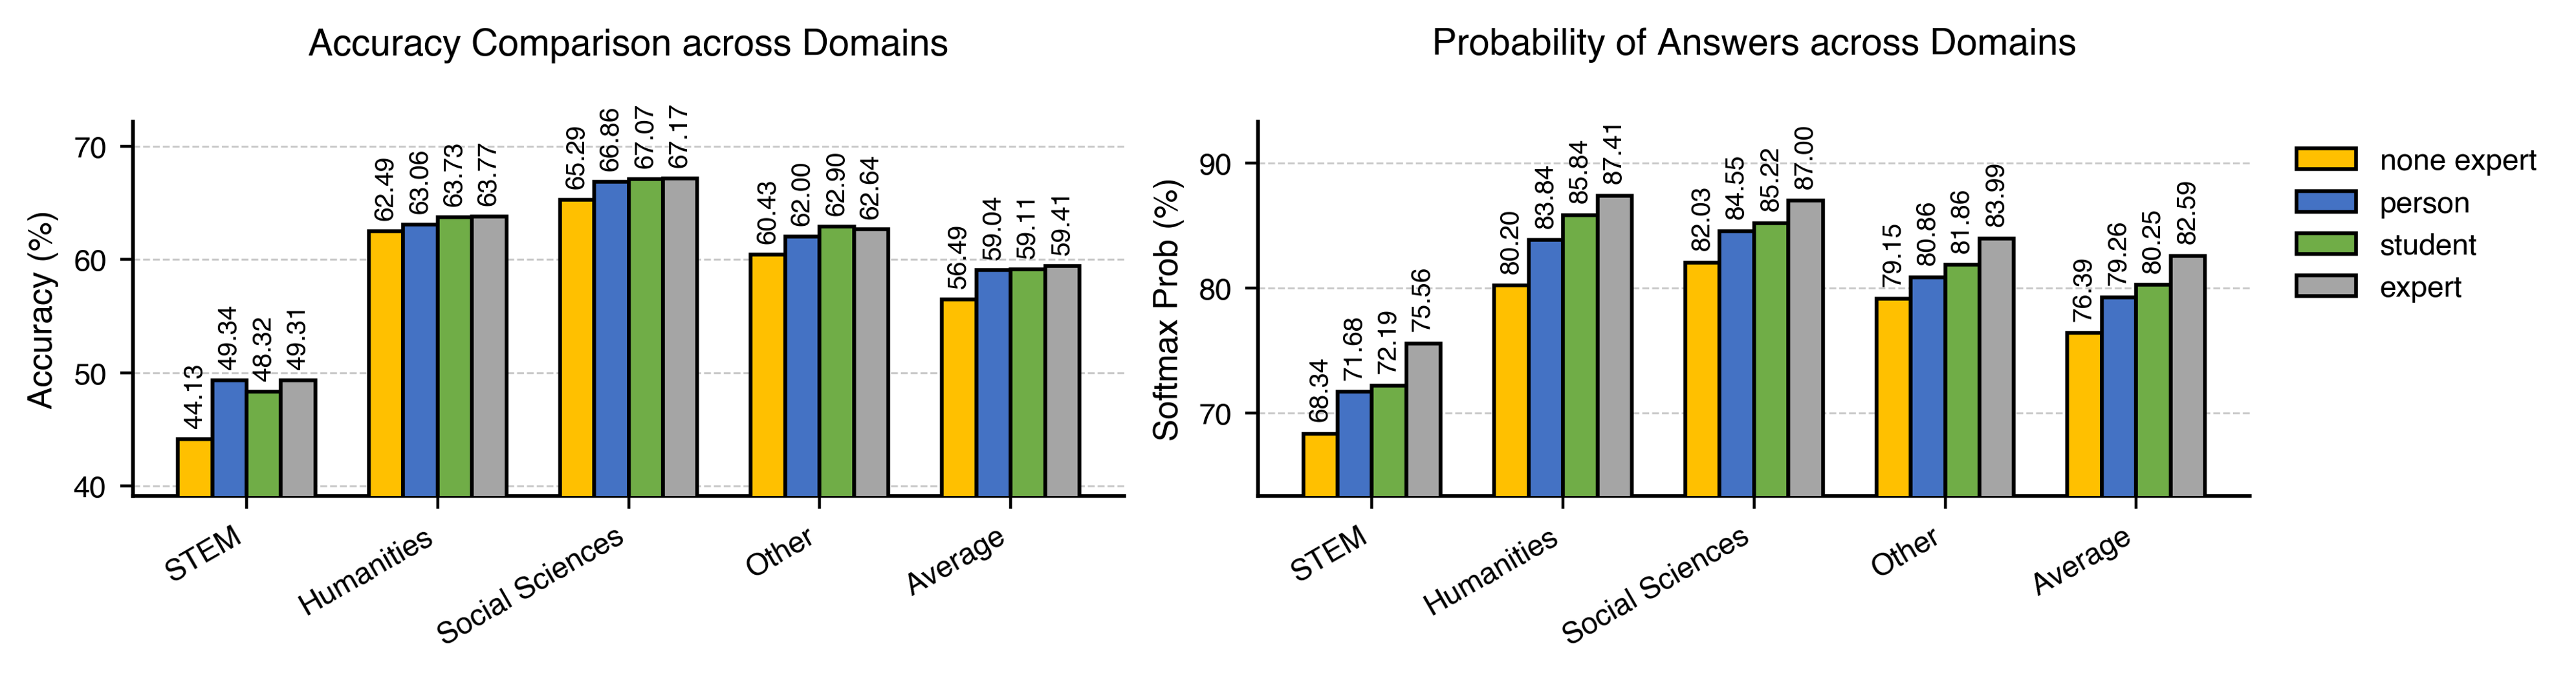
\includegraphics[width=0.95\linewidth]{figure1-4-2.png}
    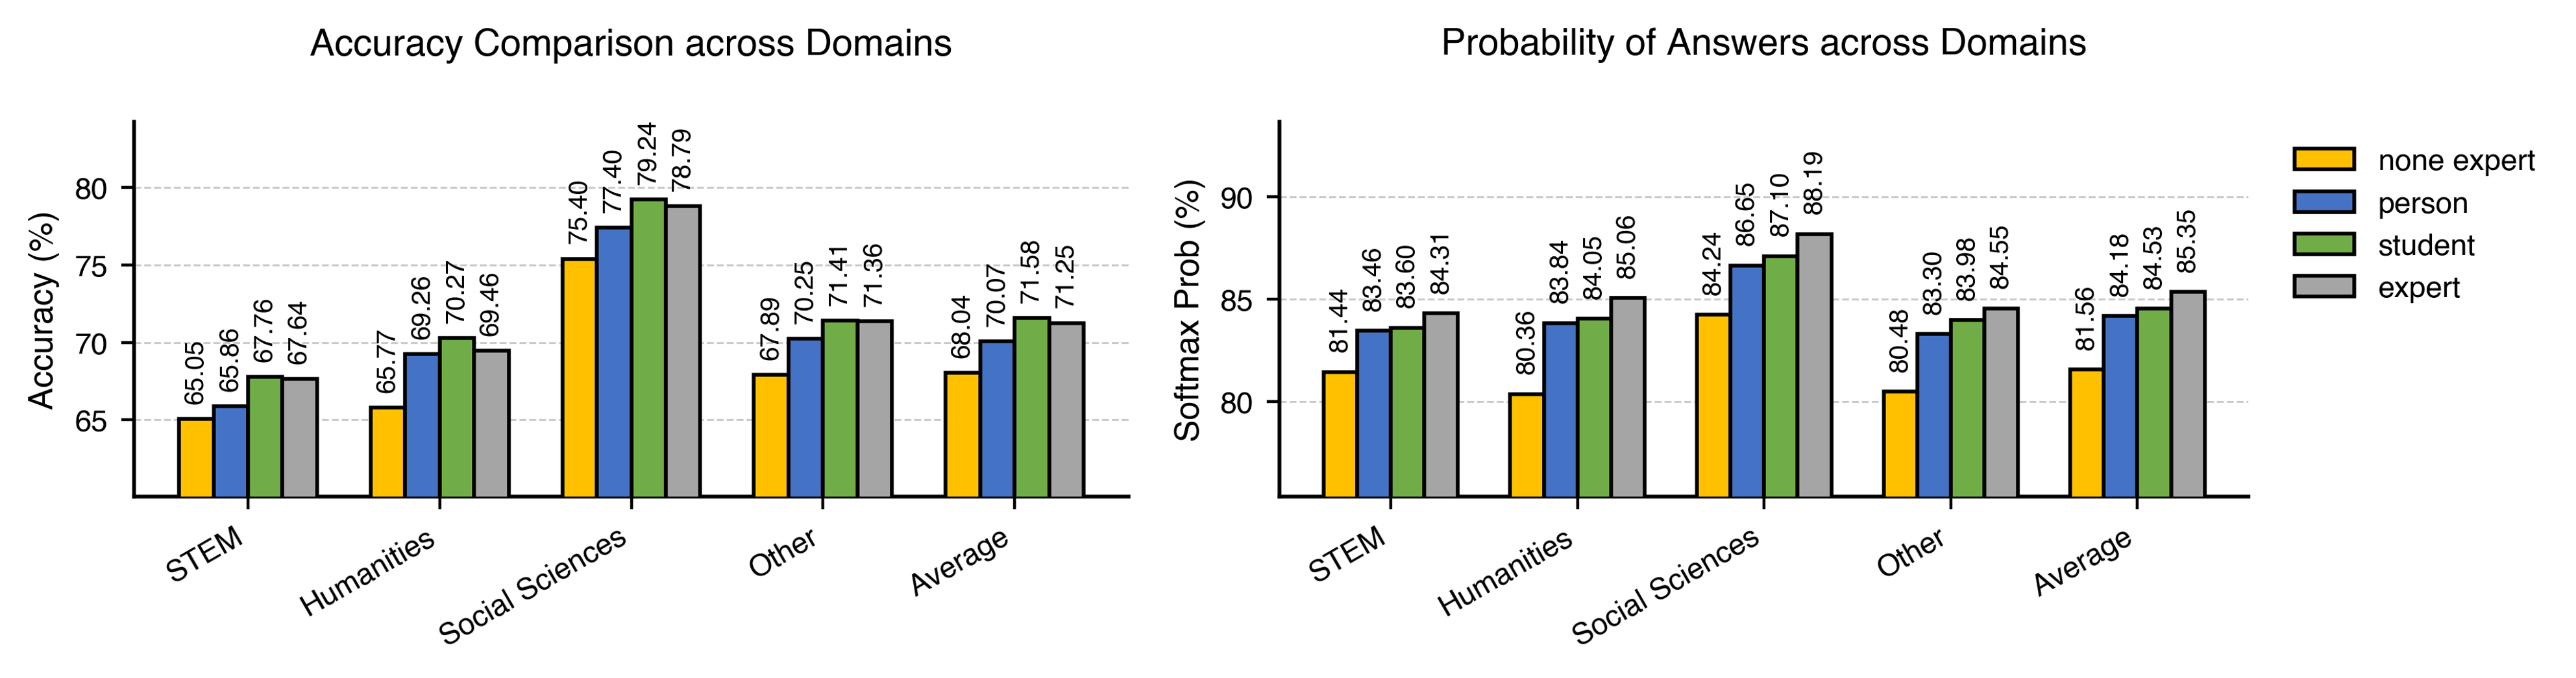
\includegraphics[width=0.95\linewidth]{figure1-5.png}
    \caption{\textbf{Cross-Model Consistency.} Accuracy (left) vs.\ confidence (right) across domains under different role prompts for \emph{Mistral-7B-IT} (top) and \emph{Qwen3-8B-IT} (bottom). Both models replicate the same trend observed in Llama3-8B-IT, highlighting the universality of role-induced confidence modulation.}
    \label{fig:app-cross-model}
\end{figure*}

\begin{figure*}[htbp]
    \centering
    \begin{minipage}{0.48\linewidth}
        \centering
        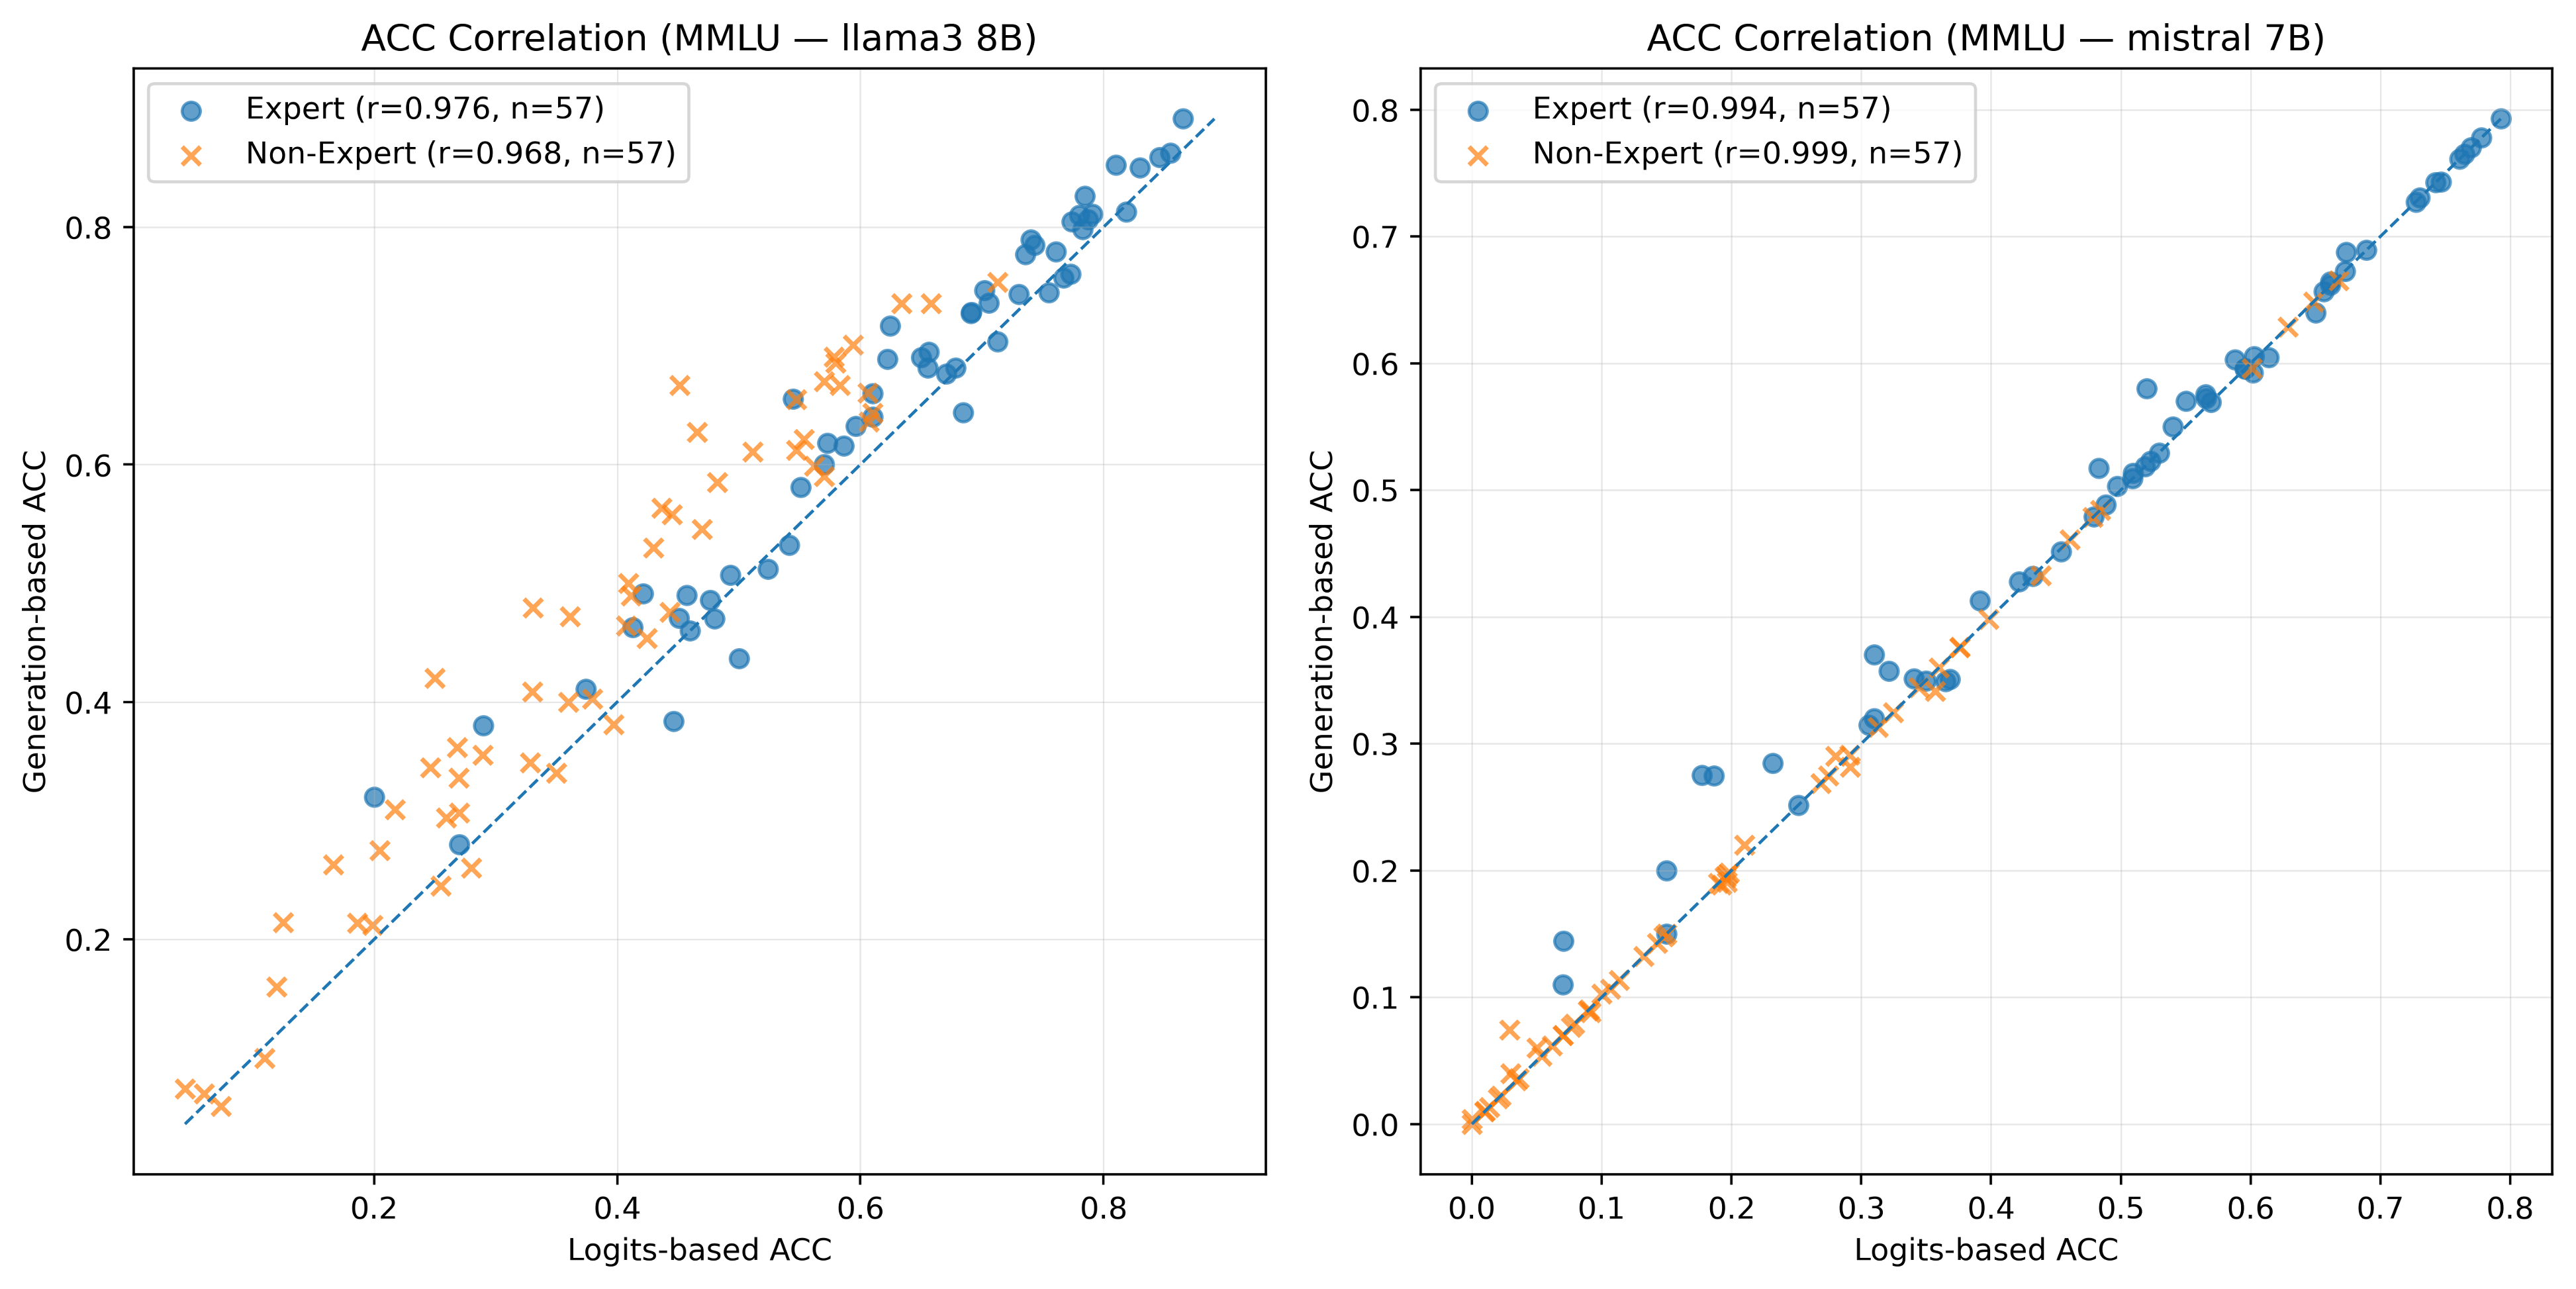
\includegraphics[width=\linewidth]{figure18.png}
        \subcaption{Accuracy Correlation}
    \end{minipage}
    \hfill
    \begin{minipage}{0.48\linewidth}
        \centering
        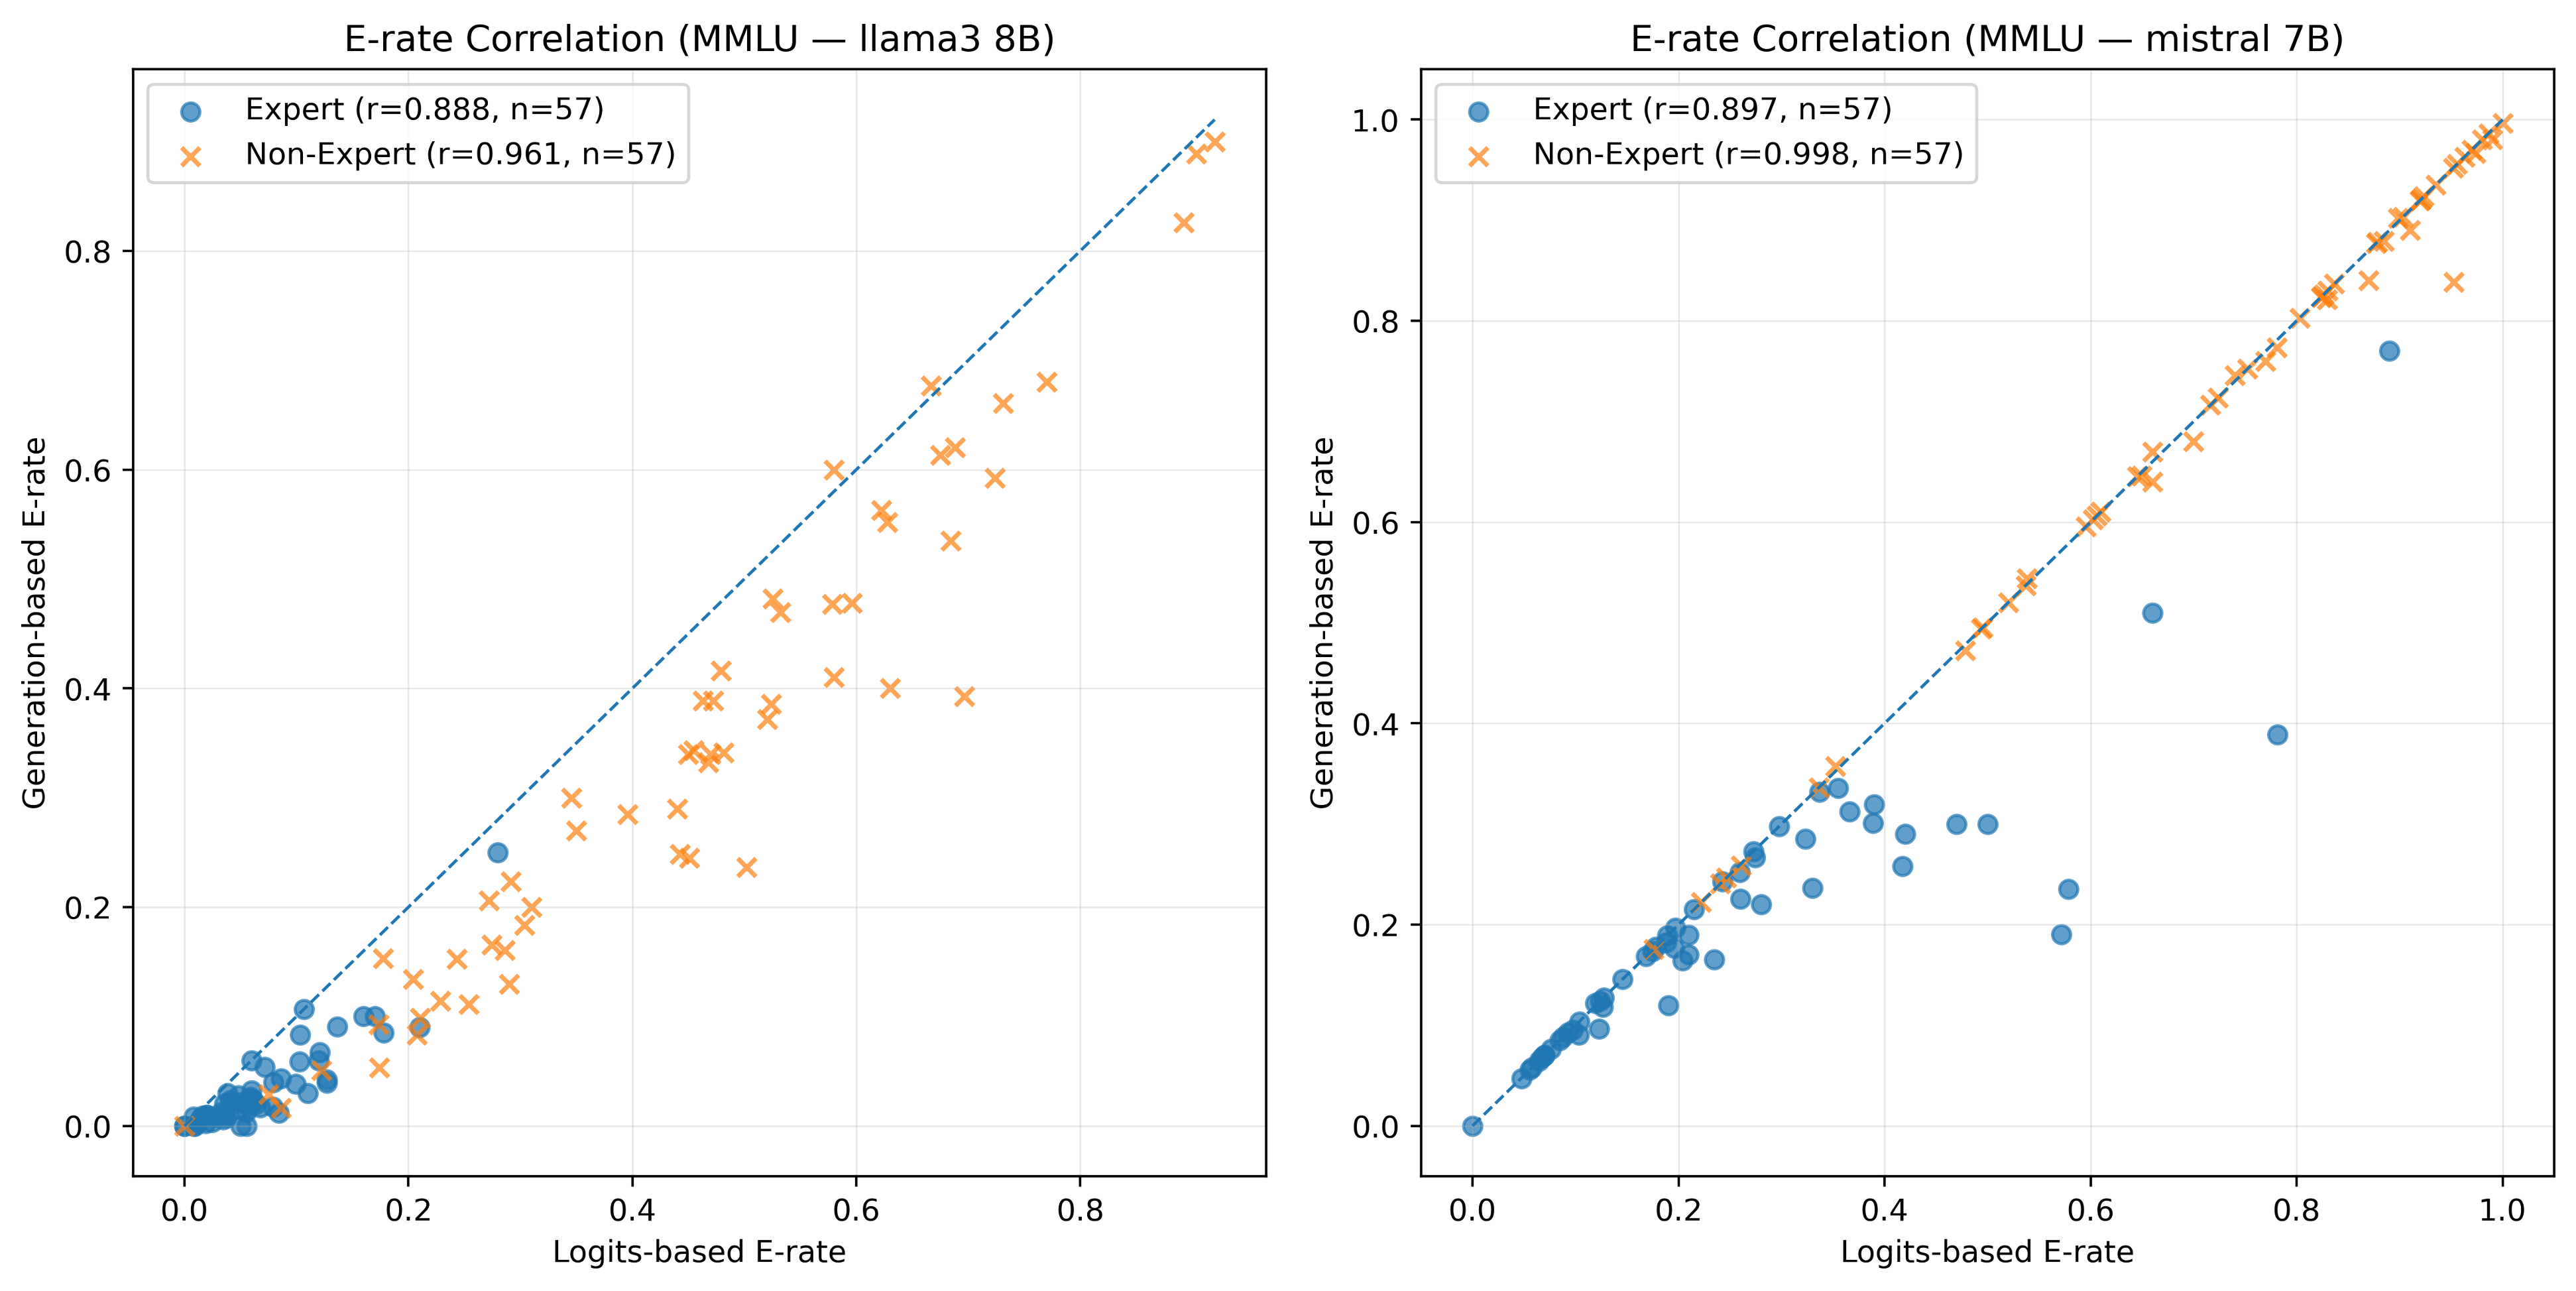
\includegraphics[width=\linewidth]{figure18_E.png}
        \subcaption{Abstention (E-ratio) Correlation}
    \end{minipage}
    \caption{Validation of Logit-Based Evaluation. Correlation between logit-based (x-axis) and generation-based (y-axis) metrics on MMLU for Llama3-8B-IT and Mistral-7B-IT. Each point represents a specific task-role pair. The high correlation ($R>0.96$) justifies our use of logits for efficient evaluation.}
    \label{fig:logit-gen-corr}
\end{figure*}

\begin{figure*}[t]
    \centering
    \begin{subfigure}{0.48\linewidth}
        \centering
        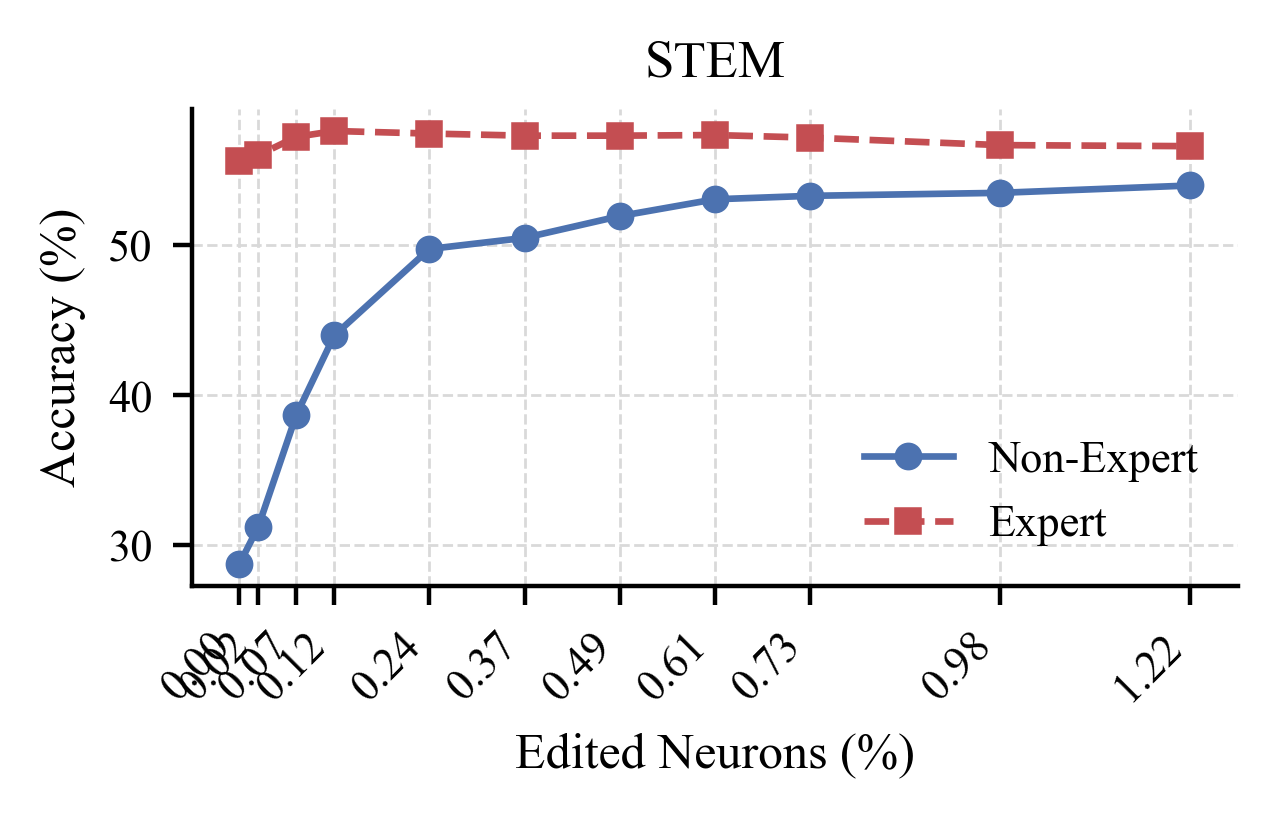
\includegraphics[width=\linewidth]{figure5-stem.png}
        \caption{STEM}
    \end{subfigure}
    \hfill
    \begin{subfigure}{0.48\linewidth}
        \centering
        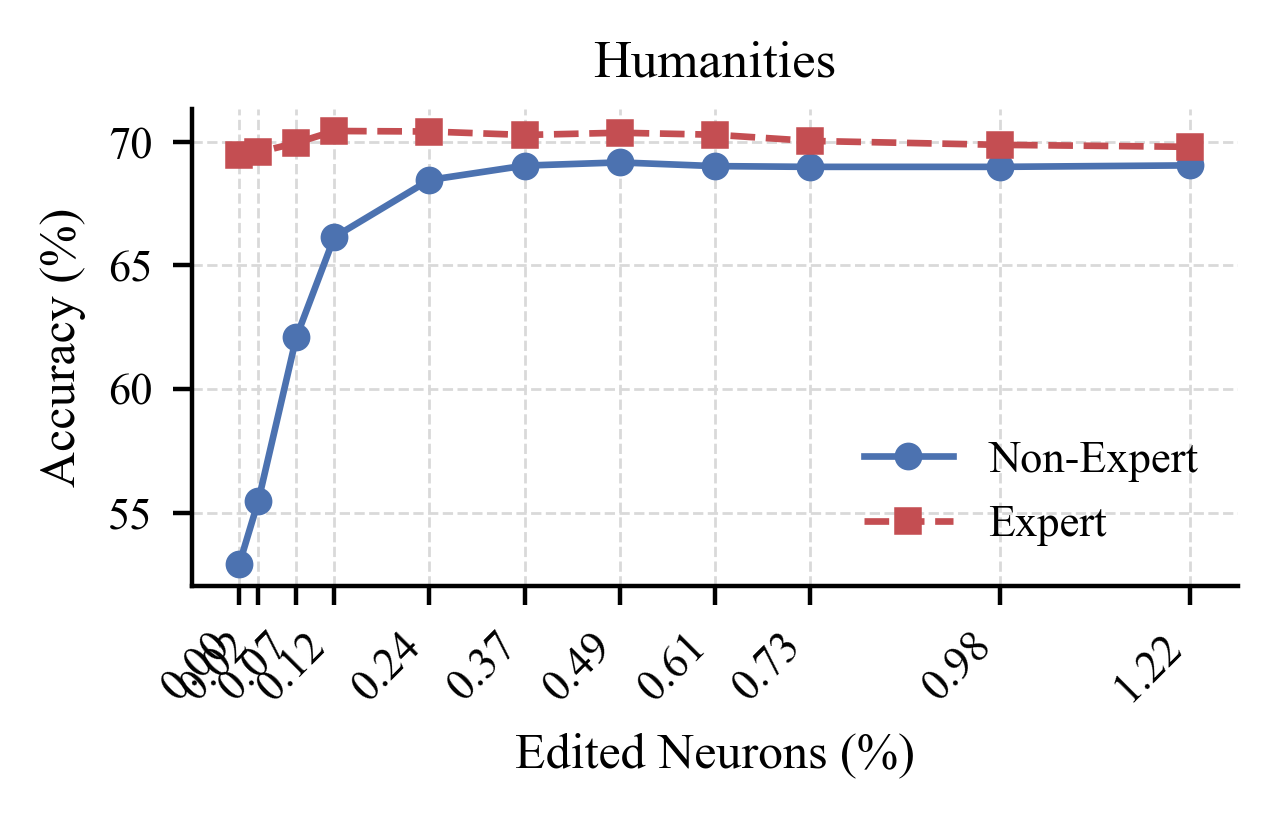
\includegraphics[width=\linewidth]{figure5-hunam.png}
        \caption{Humanities}
    \end{subfigure}

    \begin{subfigure}{0.48\linewidth}
        \centering
        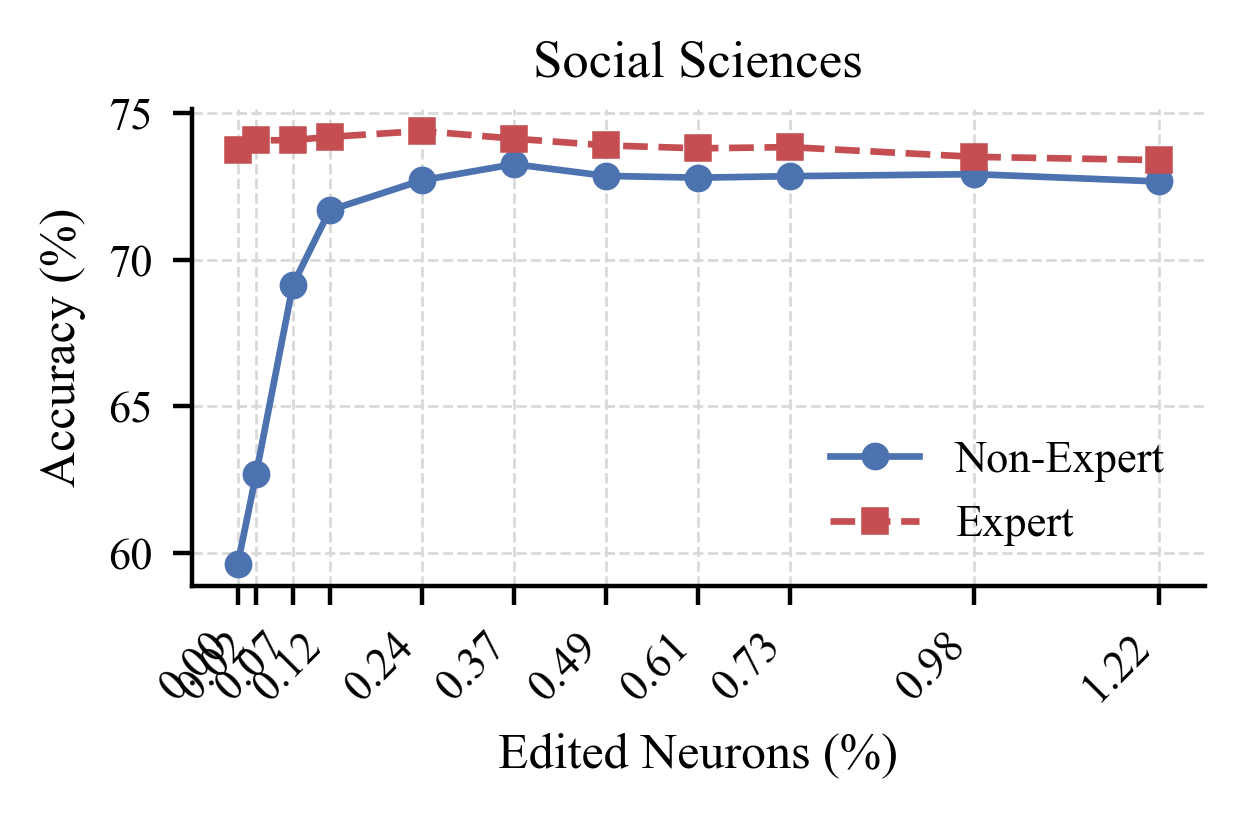
\includegraphics[width=\linewidth]{figure5-social.png}
        \caption{Social Sciences}
    \end{subfigure}
    \hfill
    \begin{subfigure}{0.48\linewidth}
        \centering
        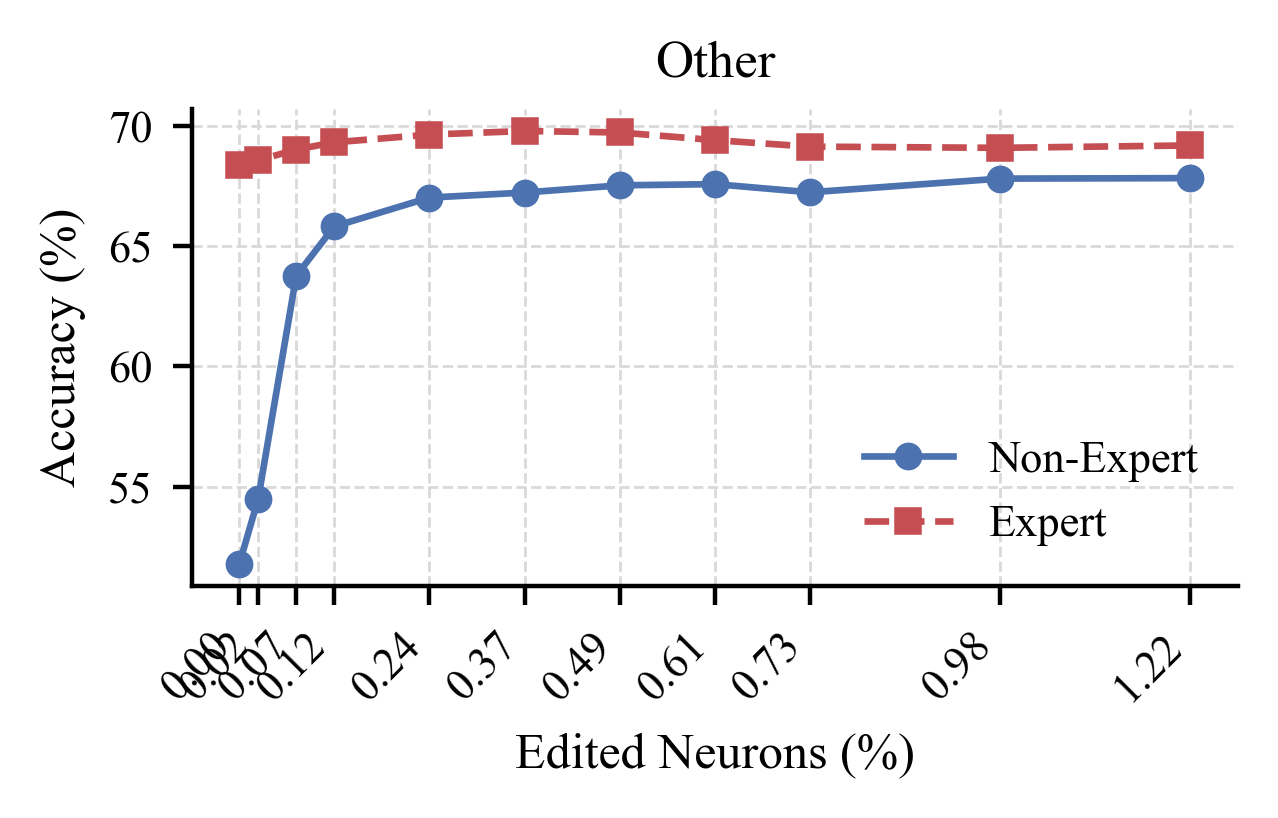
\includegraphics[width=\linewidth]{figure5-other.png}
        \caption{Other}
    \end{subfigure}

    \caption{Domain-wise Editing Sparsity. Accuracy under expert and non-expert roles across varying neuron sparsity levels ($\rho$). The overall pattern mirrors the mean trend (Figure~\ref{fig:scaling}), with non-expert gains consistently saturating around $\rho \approx 0.5\%$ across all domains, while expert performance remains steady.}
    \label{fig:domain-sparsity}
\end{figure*}


\subsection{Behavioral Analysis}
\subsubsection{Task-level Breakdown of Role Effects}
\label{app:task-breakdown}
Table~\ref{tab:example-acc-logit-appendix} provides specific examples of the dissociation between accuracy and confidence across different models and tasks.

\subsubsection{Cross-Model Consistency of Role Effects}
\label{app:cross-model-consistency}
Figure~\ref{fig:app-cross-model} presents results for \emph{Mistral-7B-IT} and \emph{Qwen3-8B-IT}, complementing the Llama3-8B-IT plots shown in the main paper. Across both models, we observe a highly consistent pattern: confidence follows a clear hierarchical gradient (\texttt{expert} > \texttt{student} > \texttt{person} > \texttt{non-expert}), whereas accuracy remains largely unchanged across domains. This confirms that the dissociation between internal certainty and output correctness is not model-specific, but a general effect of role conditioning.

\subsection{Validation: Correlation between Generation and Logits}
\label{app:logit-validation}
To validate the reliability of our evaluation protocol, we compared results computed from logits with those obtained from greedy generation. Specifically, we evaluated both accuracy and abstention (E-ratio) across tasks and roles for Llama3-8B-IT and Mistral-7B-IT.
As shown in Figure~\ref{fig:logit-gen-corr} (Left), the two evaluation methods yield nearly identical results on accuracy, with Pearson's $R$ values exceeding 0.96 across roles and models. Similarly, Figure~\ref{fig:logit-gen-corr} (Right) shows that abstention rates computed from logits strongly correlate with those from generation. These results confirm that logits-based evaluation is a faithful and computationally efficient proxy for generation-based metrics.


\begin{figure}[t]
    \centering
    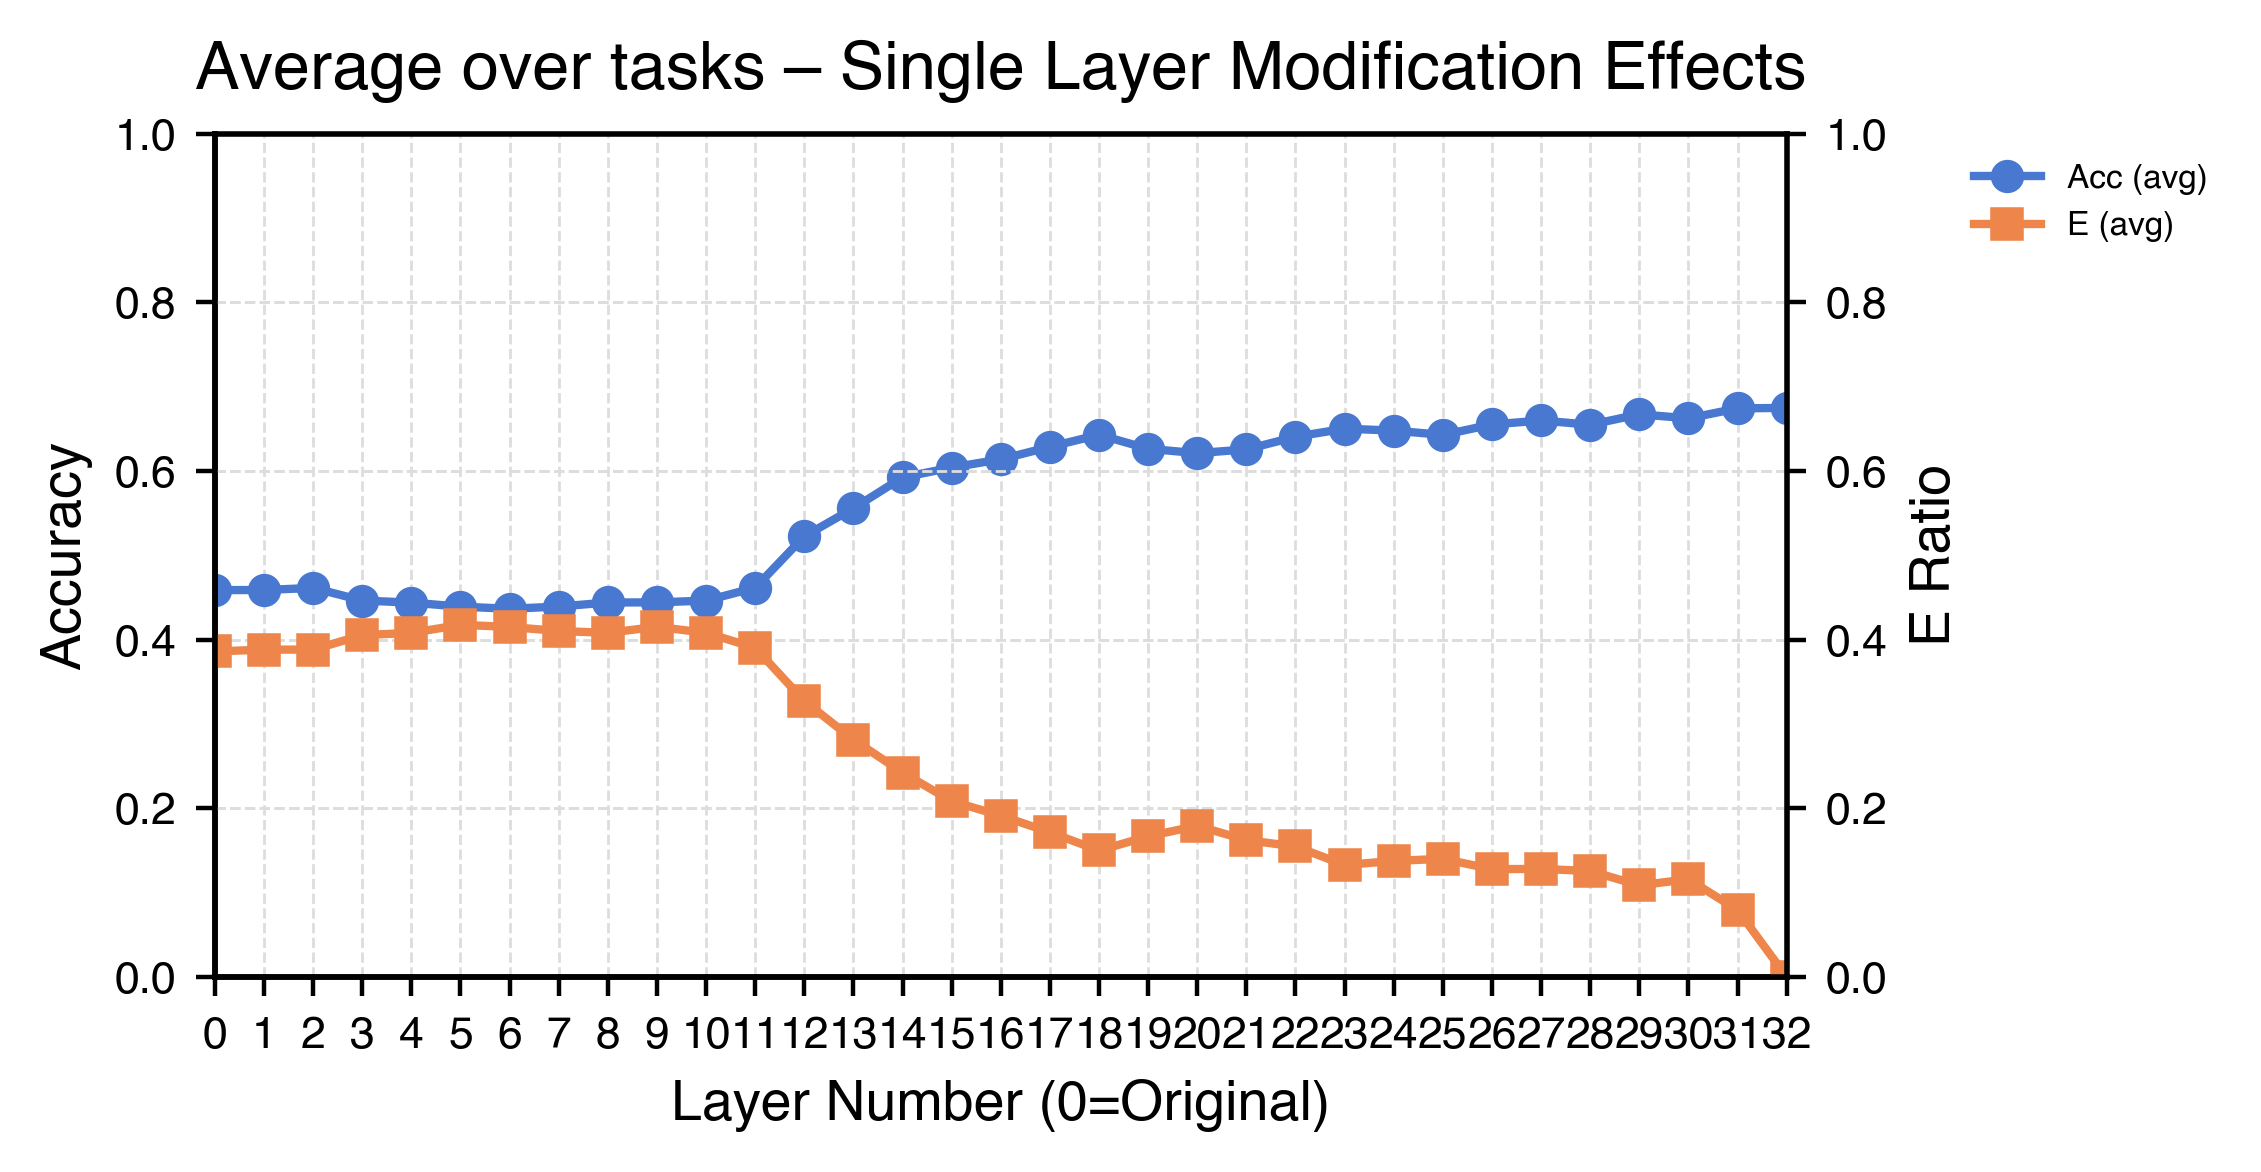
\includegraphics[width=0.95\linewidth]{figure8-2.png}
    \caption{Layer-wise Steering Effects. Average performance over four MMLU tasks on \emph{Llama3-8B-IT} using single-layer functional vector editing ($\alpha=1$). Role-sensitive effects (increased accuracy, decreased abstention) emerge distinctly around layer 11 and peak in the middle layers, corroborating our strategy to target the middle-layer RSN subspace.}
    \label{fig:single-layer-effect}
\end{figure}


\subsection{Localization: Single-Layer Functional Vector Editing}
\label{app:single-layer-editing}
To further localize role-sensitive transformations, we applied Functional Vector (FV) editing (using \emph{all neurons} in a single layer, $\alpha=1$) to Llama3-8B-IT across four representative MMLU tasks (``college computer science,'' ``US foreign policy,'' ``management,'' and ``jurisprudence''), each from a different domain.

As shown in Figure~\ref{fig:single-layer-effect}, editing effects begin to emerge around layer 11, rise steeply through the middle layers, and gradually saturate in deeper layers. This indicates that the middle layers (11--19) are the main locus where role-sensitive representations are encoded. This finding provides convergent evidence for our refined RSN design, which focuses on middle-layer edits to maximize steering efficiency while reducing interference.


\subsection{Domain-wise Effect of Neuron Editing Sparsity}
\label{app:domain-sparsity}
To further examine domain-specific variation, we plot accuracy under the \emph{expert} and \emph{non-expert} roles for each MMLU domain: STEM, Humanities, Social Sciences, and Other.
Across all domains (Figure~\ref{fig:domain-sparsity}), the \emph{non-expert} role consistently benefits from sparse neuron edits up to $\rho \approx 0.5\%$, after which performance saturates or slightly declines. The \emph{expert} role remains relatively stable, confirming that role-conditioned behavior can be selectively enhanced without degrading well-calibrated expert reasoning.

\subsection{Layer-wise Correlation For Mistral and Qwen3}
\label{app:midlayer}

To examine whether the mid-layer concentration of role-sensitive signals generalizes across architectures, we compute the layer-wise Pearson correlation between ``expert'' and ``non-expert'' hidden states in both \emph{Mistral-7B-IT} and \emph{Qwen3-8B-IT}.

As shown in Figure~\ref{fig:layer-corr-cross-model}, both models exhibit a similar three-phase pattern to \emph{Llama3-8B-IT}:
(1) early layers show nearly identical activations,
(2) middle layers diverge sharply (Mistral: layers 14--21; Qwen3: 17--25), and
(3) deeper layers partially recover.
This cross-model consistency suggests that role-specific transformations are robustly localized to middle layers across diverse transformer architectures.


\begin{figure}[t]
    \centering
    \begin{subfigure}{0.9\linewidth}
        \centering
        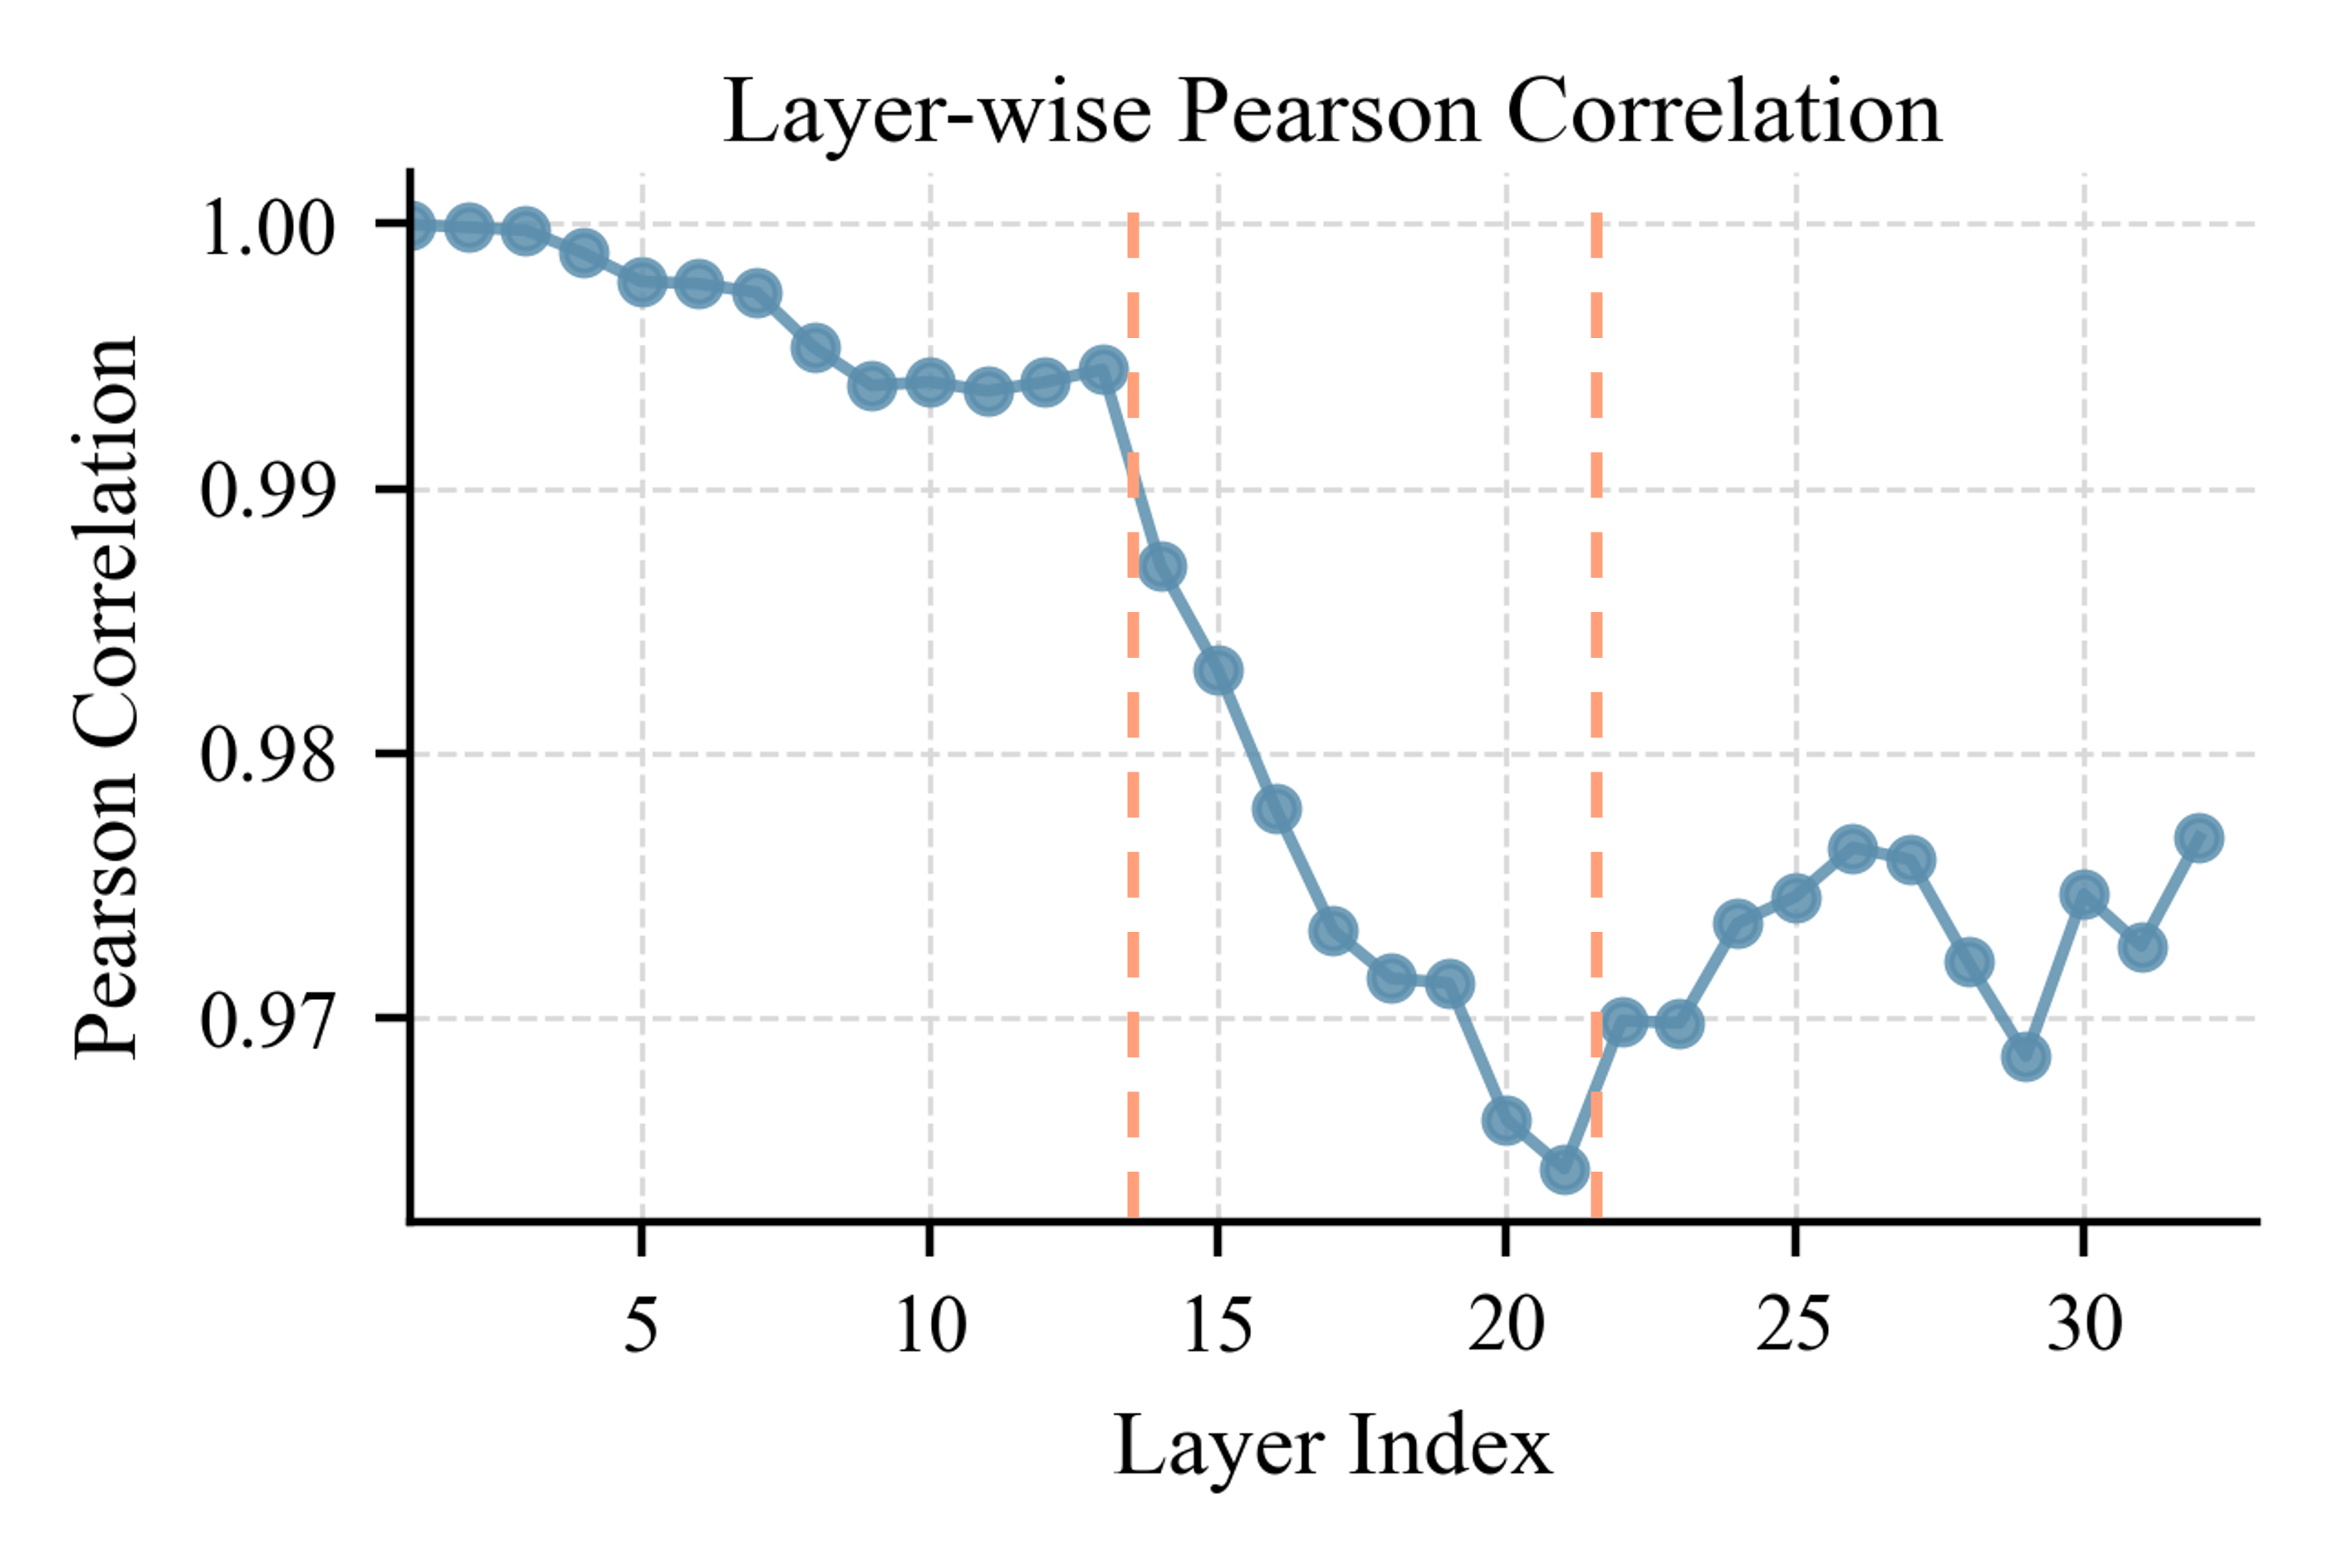
\includegraphics[width=\linewidth]{figure6-mistral.png}
        \caption{Mistral-7B-IT: Divergence peaks at layers 14--21.}
    \end{subfigure}

    \begin{subfigure}{0.9\linewidth}
        \centering
        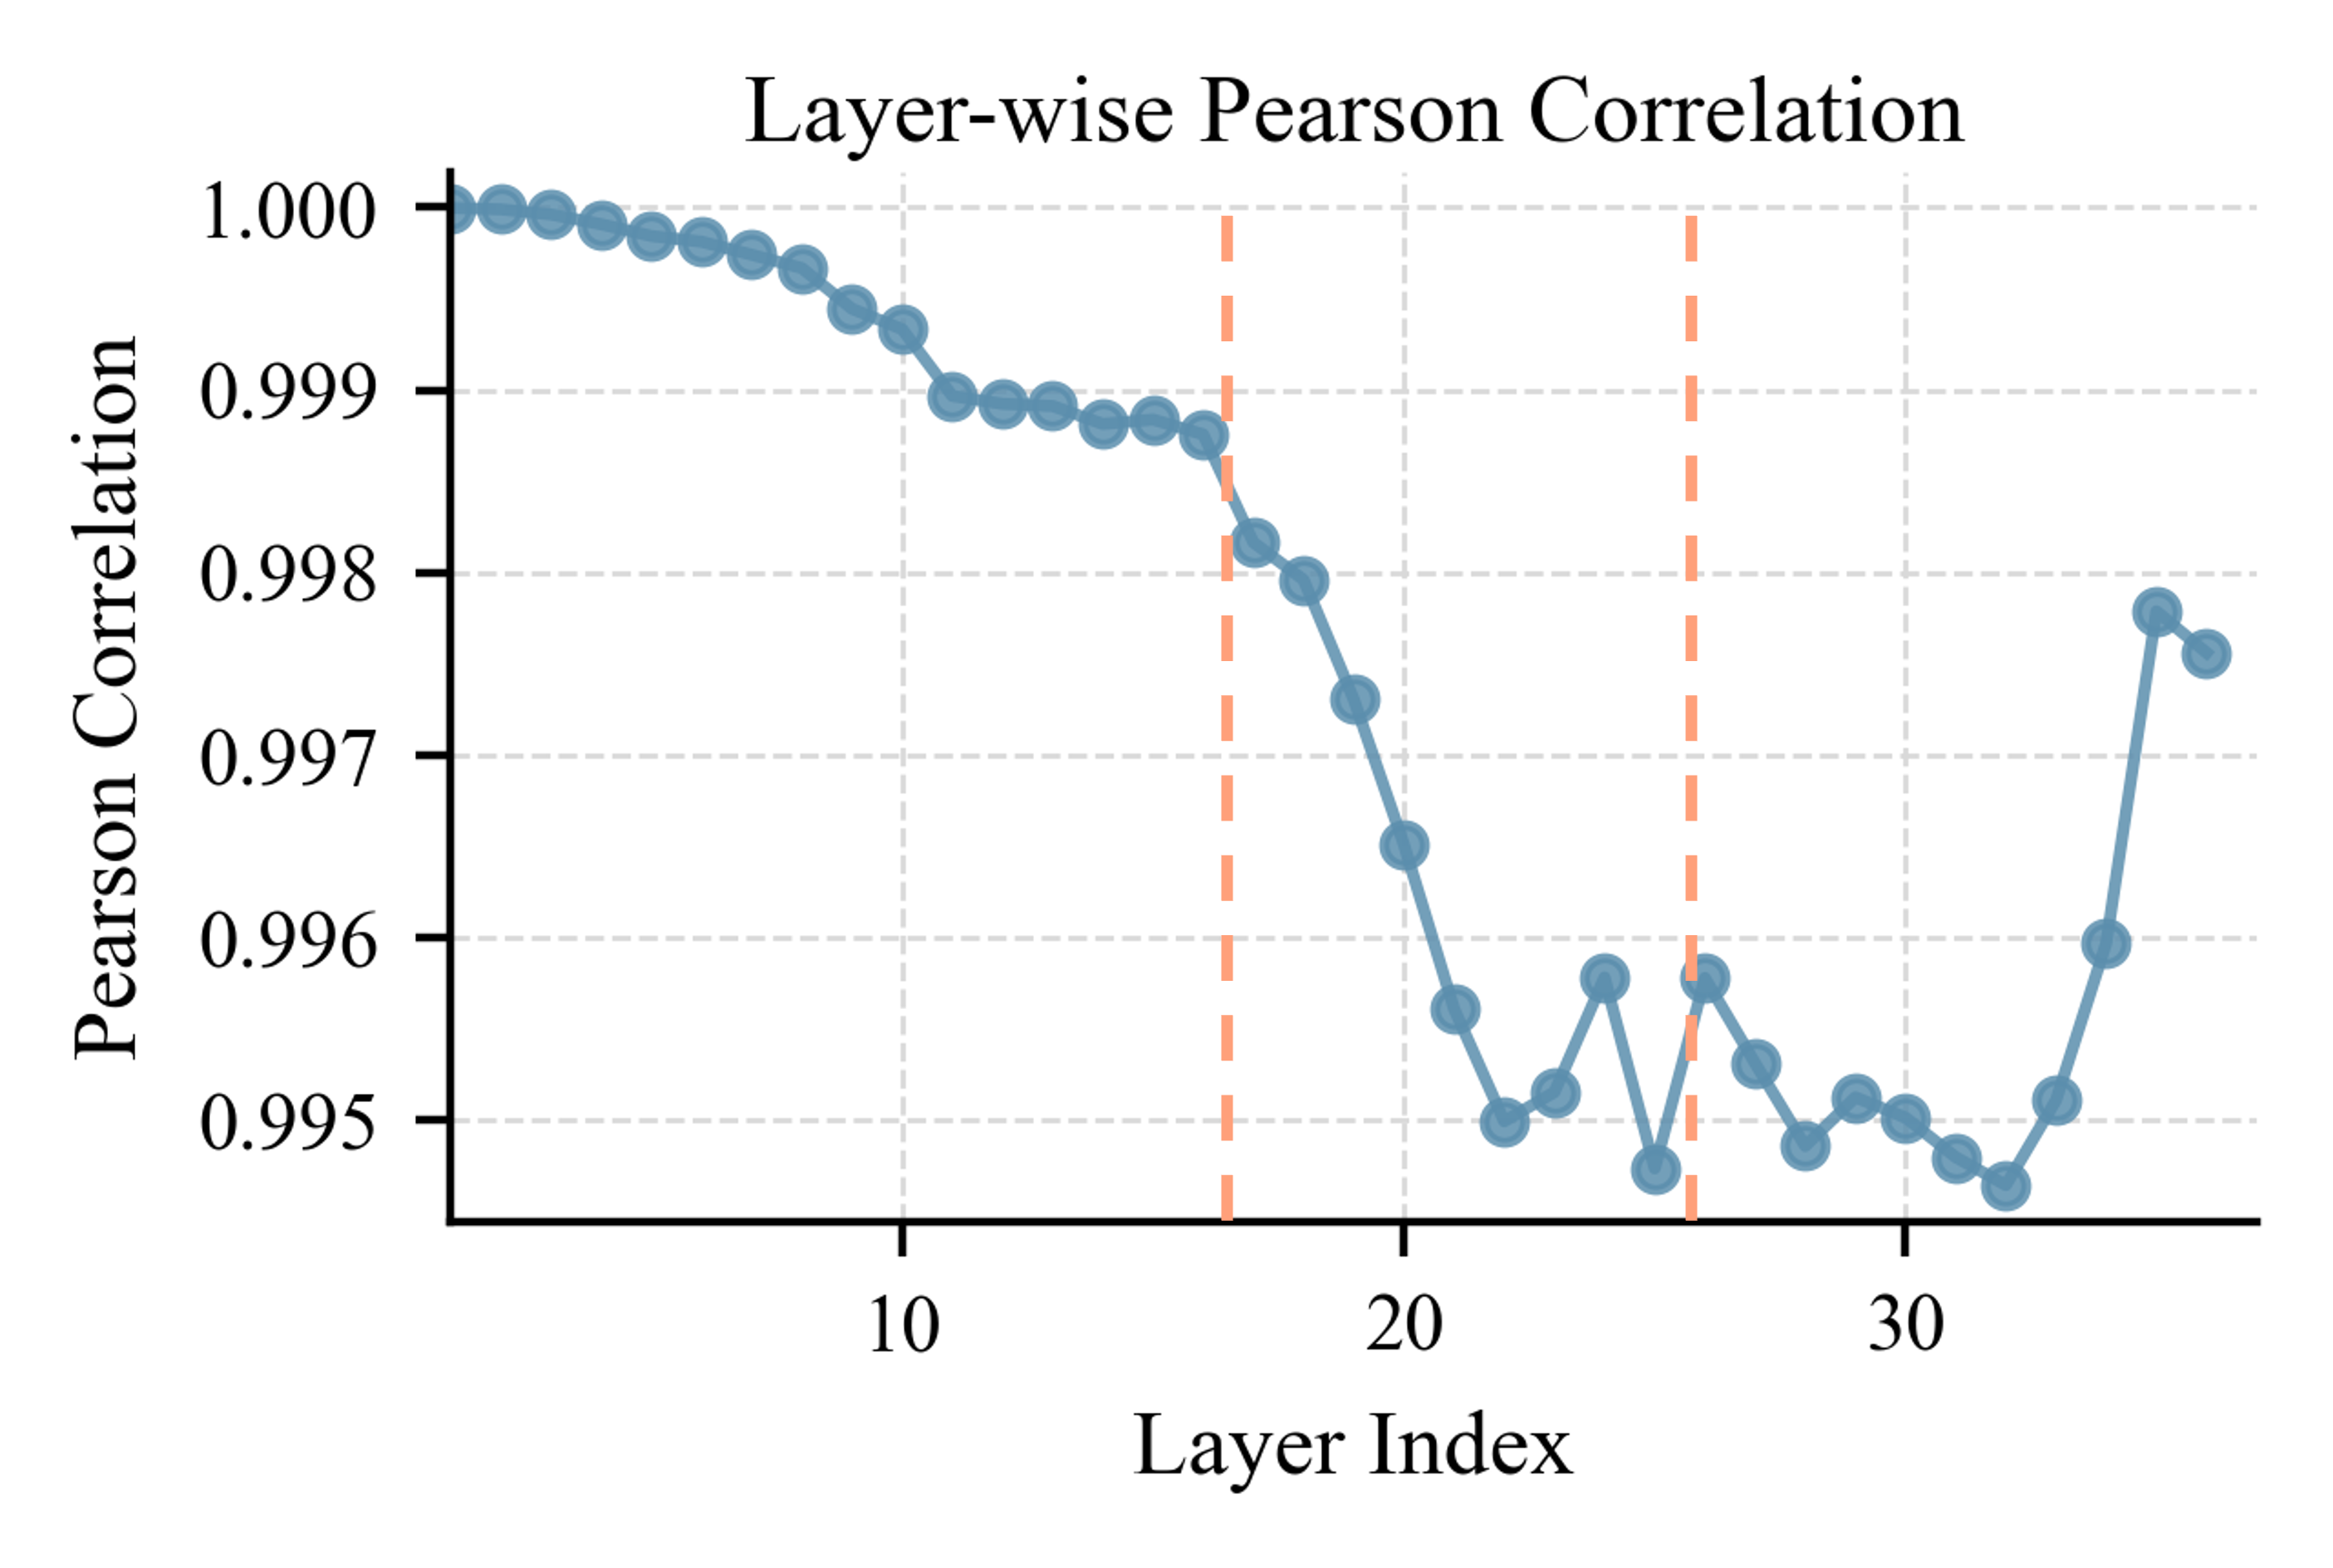
\includegraphics[width=\linewidth]{figure6-qwen3.png}
        \caption{Qwen3-8B-IT: Divergence peaks at layers 17--25.}
    \end{subfigure}

    \caption{Cross-Model Layer-wise Correlation. Pearson correlation between ``expert'' and ``non-expert'' hidden states. Both models replicate the mid-layer divergence pattern observed in \emph{Llama3-8B-IT} (Figure~\ref{fig:localization}).}
    \label{fig:layer-corr-cross-model}
\end{figure}

\begin{table}[htbp]
\centering
\caption{Generalization on Mistral-7B-IT (ARC-E). RSN editing ($L_{14-22}, \alpha{=}4$) significantly reduces abstention and recovers accuracy across generic roles, replicating the mechanism observed in Llama3.}
\label{tab:app-mistral-arc}
\setlength{\tabcolsep}{8pt}
\renewcommand{\arraystretch}{1.0}
\small
\begin{tabular}{l c c c c}
\toprule
\textbf{Role}
& \multicolumn{2}{c}{\textbf{Accuracy}} 
& \multicolumn{2}{c}{\textbf{E-ratio}} \\
\cmidrule(lr){2-3} \cmidrule(lr){4-5}
& Orig. & Edit. & Orig. & Edit. \\
\midrule
Non-Exp.   & 22.55 & \textbf{46.76} & 73.86 & \textbf{44.71} \\
Person     & 45.48 & \textbf{52.51} & 44.63 & \textbf{36.72} \\
Student    & 48.03 & \textbf{59.96} & 41.93 & \textbf{29.38} \\
Expert     & 63.86 & \textbf{80.54} & 19.69 & \textbf{3.01} \\
L0 Exp.    & 37.57 & \textbf{60.66} & 53.98 & \textbf{29.42} \\
L1 Exp.    & 64.86 & \textbf{80.19} & 16.95 & \textbf{4.25} \\
L2 Exp.    & 65.37 & \textbf{81.39} & 15.87 & \textbf{2.24} \\
L3 Exp.    & 65.52 & \textbf{81.54} & 15.79 & \textbf{1.85} \\
\bottomrule
\end{tabular}
\end{table}

\begin{table}[htbp]
\centering
\caption{Performance on CommonSenseQA (CSQA-E). RSN editing ($\alpha=4$) consistently unlocks performance in weaker roles while maintaining high accuracy in expert roles across both Llama3-8B-IT and Mistral-7B-IT.}
\label{tab:csqa-results}
\setlength{\tabcolsep}{3pt}
\renewcommand{\arraystretch}{1.0}
\small
\begin{tabular}{l l c c c c}
\toprule
\multirow{2}{*}{\textbf{Model}} & \multirow{2}{*}{\textbf{Role}}
& \multicolumn{2}{c}{\textbf{Accuracy (\%)}} 
& \multicolumn{2}{c}{\textbf{E-ratio (\%)}} \\
\cmidrule(lr){3-4} \cmidrule(lr){5-6}
& & Orig. & Edit. & Orig. & Edit. \\
\midrule
\multirow{8}{*}{\textbf{Llama3}}& Non-Exp.   & 62.90 & \textbf{72.73} & 14.99 & \textbf{0.25} \\
& Person     & 47.50 & \textbf{72.65} & 36.36 & \textbf{0.57} \\
& Student    & 53.48 & \textbf{72.73} & 28.01 & \textbf{0.08} \\
& Expert     & 71.91 & \textbf{73.96} &  5.00 & \textbf{0.16} \\
& L0 Exp.    & 52.66 & \textbf{72.73} & 30.71 & \textbf{0.25} \\
& L1 Exp.    & 72.56 & \textbf{72.81} &  3.28 & \textbf{0.08} \\
& L2 Exp.    & \textbf{74.28} & 73.46 &  1.31 & \textbf{0.08} \\
& L3 Exp.    & \textbf{74.20} & 72.97 &  1.56 & \textbf{0.08} \\
\midrule
\multirow{8}{*}{\textbf{Mistral}}
& Non-Exp.   & 30.79 & \textbf{57.25} & 61.43 & \textbf{19.00} \\
& Person     & 57.90 & \textbf{66.01} & 22.11 & \textbf{4.18} \\
& Student    & 57.82 & \textbf{66.18} & 22.60 & \textbf{4.91} \\
& Expert     & 60.28 & \textbf{67.90} & 20.07 & \textbf{1.80} \\
& L0 Exp.    & 47.58 & \textbf{63.72} & 37.59 & \textbf{6.80} \\
& L1 Exp.    & 62.16 & \textbf{66.75} & 16.05 & \textbf{1.97} \\
& L2 Exp.    & 62.00 & \textbf{67.32} & 16.54 & \textbf{2.05} \\
& L3 Exp.    & 61.67 & \textbf{67.16} & 16.63 & \textbf{2.21} \\
\bottomrule
\end{tabular}
\end{table}

\subsection{Extended Cross-Domain Generalization Results}
\label{app:generalization-extended}

This section provides supporting evidence for the cross-domain robustness of RSNs discussed in Section~\ref{sec:cross-domain}. We present two complementary analyses: (1) the generalization of Mistral-7B-IT on the \emph{ARC Challenge}, and (2) the performance of both Llama3 and Mistral on \emph{CommonSenseQA} (CSQA).

\paragraph{Mistral-7B-IT on ARC-E.}
Table~\ref{tab:app-mistral-arc} details the performance of Mistral-7B-IT on ARC-E using generic roles. Consistent with Llama3, Mistral exhibits a strong response to RSN editing ($L_{14-22}, \alpha{=}4$). In the \emph{Non-Expert} role, accuracy doubles (22.55\% $\to$ 46.76\%) as the model overcomes its extreme conservatism, confirming that the gain control mechanism functions across different model architectures.

\paragraph{CommonSenseQA Analysis (CSQA-E).}
Table~\ref{tab:csqa-results} reports results on \emph{CommonSenseQA} (CSQA-E) for both models. Consistent with ARC findings, RSN editing improves accuracy and calibration across all roles. The effect is most pronounced for weaker roles (\emph{non-expert}, \emph{student}), where abstention is drastically reduced. For stronger expert roles, RSNs continue to reduce residual uncertainty (E-ratio), verifying that RSNs generalize not only across tasks (Scientific vs. Commonsense) but also across diverse role phrasings.

\subsection{Generalization Across Prompt Formats}
\label{app:prompt-generalization}
To verify that RSN-based steering is not tied to specific prompt wordings, we evaluate model behavior under differing prompt formulations. All experiments use the abstention-enabled variant (with ``E) I am not sure''), and apply the same refined middle-layer RSNs from the main experiments ($\text{RSNs}_{[11,19]}$ for Llama3-8B-IT, $\alpha{=}3$ or $4$).

\subsubsection{Vanilla Instruction Format}
We first replace the standard role template with a plain instruction-style prompt, stripping away descriptive framing:
\begin{quote}
\small
\ttfamily
What is a normative perspective?\\
A) The way things are.\\
...\\
E) I am not sure.\\
\textnormal{\textit{As an honest (non) [task] expert, answer:}}
\end{quote}

As shown in Table~\ref{tab:prompt-generalization} (Panel A), RSN editing substantially improves both accuracy and decisiveness under this minimal instruction format. Even without contextual hints, the refined RSNs—derived from a different prompt formulation—yield consistent gains across all domains.

\subsubsection{Chat-Template Format}
Next, we evaluate RSN steering under a chat-template format, where role instructions are injected into the system message:
\begin{quote}
\small
\ttfamily
\textbf{System:} Now you are a \emph{(non) [task] expert}.\\
\textbf{User:} Would you answer the following question with A, B, C, D or E?
Question: ...\\
Your answer among ``A, B, C, D, E'' is:
\end{quote}
As shown in Table~\ref{tab:prompt-generalization} (Panel B), RSN steering generalizes robustly to chat-formatted contexts. Middle-layer RSNs produce large accuracy gains with near-zero abstention, indicating that the steering effect persists under dialogue-style prompting.

Taken together, these findings demonstrate that RSNs capture latent role representations intrinsic to model computation rather than superficial textual cues.

\begin{table*}[htbp]
\centering
\caption{Robustness to Prompt Formats (Llama3-8B-IT). RSN steering effectively modulates confidence across (A) Vanilla Instruction and (B) Chat Template formats. The mechanism generalizes beyond the specific wording used for neuron discovery.}
\label{tab:prompt-generalization}
\setlength{\tabcolsep}{5pt}
\renewcommand{\arraystretch}{1.05}
\small
\begin{tabular}{l c c c c c c}
\toprule
\textbf{Condition} & \textbf{STEM} & \textbf{Humanities} & \textbf{Social Sci.} & \textbf{Other} & \textbf{Avg. Acc} & \textbf{E (\%)} \\
\midrule
\multicolumn{7}{l}{\textit{\textbf{Panel A: Vanilla Instruction Format}}} \\
Non-Expert (Baseline) & 17.9 & 25.4 & 37.2 & 29.9 & 26.4 & 53.8 \\
+ RSN $\alpha=3$      & 31.0 & 40.0 & 45.9 & 41.3 & 38.5 & 23.1 \\
+ RSN $\alpha=4$      & 36.3 & 43.3 & 46.2 & 44.4 & 41.8 & 8.3 \\
\cmidrule(lr){1-7}
Expert (Baseline)     & 33.8 & 48.8 & 51.8 & 44.5 & 43.4 & 22.9 \\
+ RSN $\alpha=3$      & 40.1 & 53.4 & 51.8 & 49.9 & 47.8 & 6.0 \\
+ RSN $\alpha=4$      & 40.4 & 49.9 & 50.1 & 48.0 & 46.3 & 2.0 \\
\midrule
\multicolumn{7}{l}{\textit{\textbf{Panel B: Chat-Template Format}}} \\
Non-Expert (Baseline) & 40.2 & 62.3 & 63.5 & 61.2 & 54.9 & 18.0 \\
+ RSN $\alpha=3$      & 51.7 & 66.6 & 67.8 & 64.3 & 61.4 & 1.0 \\
+ RSN $\alpha=4$      & 50.7 & 65.6 & 68.1 & 63.3 & 60.7 & 0.3 \\
\cmidrule(lr){1-7}
Expert (Baseline)     & 49.0 & 64.1 & 67.1 & 63.9 & 59.6 & 5.9 \\
+ RSN $\alpha=3$      & 52.7 & 66.5 & 68.2 & 64.4 & 61.8 & 0.3 \\
+ RSN $\alpha=4$      & 50.8 & 65.7 & 68.3 & 63.5 & 60.8 & 0.1 \\
\bottomrule
\end{tabular}
\end{table*}

\subsection{Benchmark Descriptions}
\label{app:datasets}
We evaluate the effects of RSN editing on other representative benchmarks besides MMLU, that do not include an explicit abstention option.  These datasets cover a broad spectrum of cognitive demands, including \emph{(i) general reasoning ability} (MMLU, MMLU-Pro, GPQA), \emph{(ii) pure logical inference} (AR-LSAT, LogiQA), \emph{(iii) factual recall and truthfulness} (TruthfulQA, FACTOR).

\begin{itemize}
    \item \textbf{MMLU-Pro}~\cite{wang2024mmlupro}: a more challenging extension of MMLU that emphasizes multi-step and compositional reasoning, featuring up to 9--10 options per question and improved robustness to prompt variation. We use the official \texttt{test} split for evaluation.
    \item \textbf{GPQA}~\cite{rein2024gpqa}: a graduate-level science benchmark spanning physics, biology, and chemistry, designed to test conceptual understanding and cross-disciplinary reasoning. We use the \texttt{main} and \texttt{diamond} subsets, merging them into a unified pool and constructing 4-option multiple-choice questions by combining the correct answer with three provided distractors in randomized order.
    \item \textbf{AR-LSAT}~\cite{zhong2021arlsat}: a law-domain reasoning dataset modeled after LSAT analytical reasoning, evaluating abstract reasoning and analogical logic under structured constraints. We use the full dataset released on GitHub.
    \item \textbf{LogiQA}~\cite{liu2021logiqa}: a reading-comprehension–style logical reasoning benchmark focused on deductive and causal inference, testing a model’s ability to apply rule-based logic to natural language contexts. We use the official \texttt{test} split from the LogiQA2.0 release on GitHub.
    % \item \textbf{PubMedQA}~\cite{jin2019pubmedqa}: a biomedical question-answering dataset built from PubMed abstracts, framed as 3-choice (Yes/No/Maybe) classification to evaluate medical reasoning and evidence-based factual recall.
    % \item \textbf{MedQA}~\cite{yang2024llmmedqa}: a large-scale biomedical question-answering benchmark derived from medical licensing examinations, testing factual understanding and clinical reasoning across multiple specialties. We use the English \texttt{source} version (\texttt{test} split) on HuggingFace, formatted as multiple-choice questions with 4–5 options.
    \item \textbf{TruthfulQA}~\cite{lin2022truthfulqa}: a benchmark evaluating factual accuracy against common misconceptions and hallucinations. We reformulate both MC1 and MC2 variants into a unified multiple-choice format, synchronously shuffling options and labels for each sample to ensure consistent randomization across runs.
    \item \textbf{FACTOR}~\cite{muhlgay2024factor}: a factual consistency benchmark comprising \emph{wiki}, \emph{news}, and \emph{expert} splits, designed to measure whether model-generated statements align with known facts and avoid internal contradictions. For each example, we place the correct answer first and concatenate it with up to three contradicted statements to form a multiple-choice question. The options are then deterministically shuffled to ensure reproducible evaluation.
\end{itemize}

\subsection{Conditional Accuracy Analysis}
\label{app:conditional-acc-table}

Table~\ref{tab:conditional-acc-appendix} details the trade-off between coverage and precision. The Non-Expert baseline is highly precise but overly conservative. RSN steering relaxes this threshold to match the Expert profile.

\begin{table}[htbp]
\centering
\small
\caption{Micro-Dynamics of Confidence (Llama3-8B-IT). RSN injection shifts the Non-Expert from an over-conservative, high-precision profile toward the Expert's decisive balance of coverage and accuracy.}
\label{tab:conditional-acc-appendix}
\setlength{\tabcolsep}{5pt}
\begin{tabular}{l c c c}
\toprule
\textbf{Config} & \textbf{Total Acc} & \textbf{E-ratio} & \textbf{Cond. Acc} \\
\midrule
\textbf{Non-Exp.}& 38.65 & 44.77 & \textbf{69.33} \\
\textbf{+4$RSN_{mid}$}& \textbf{63.22} & \textbf{3.73} & 65.45 \\
\textit{Expert Ref.}& \textit{63.01} & \textit{6.87} & \textit{67.22} \\
\bottomrule
\end{tabular}
\end{table}

\begin{figure}[t]
    \centering
    \begin{subfigure}{0.9\linewidth}
        \centering
        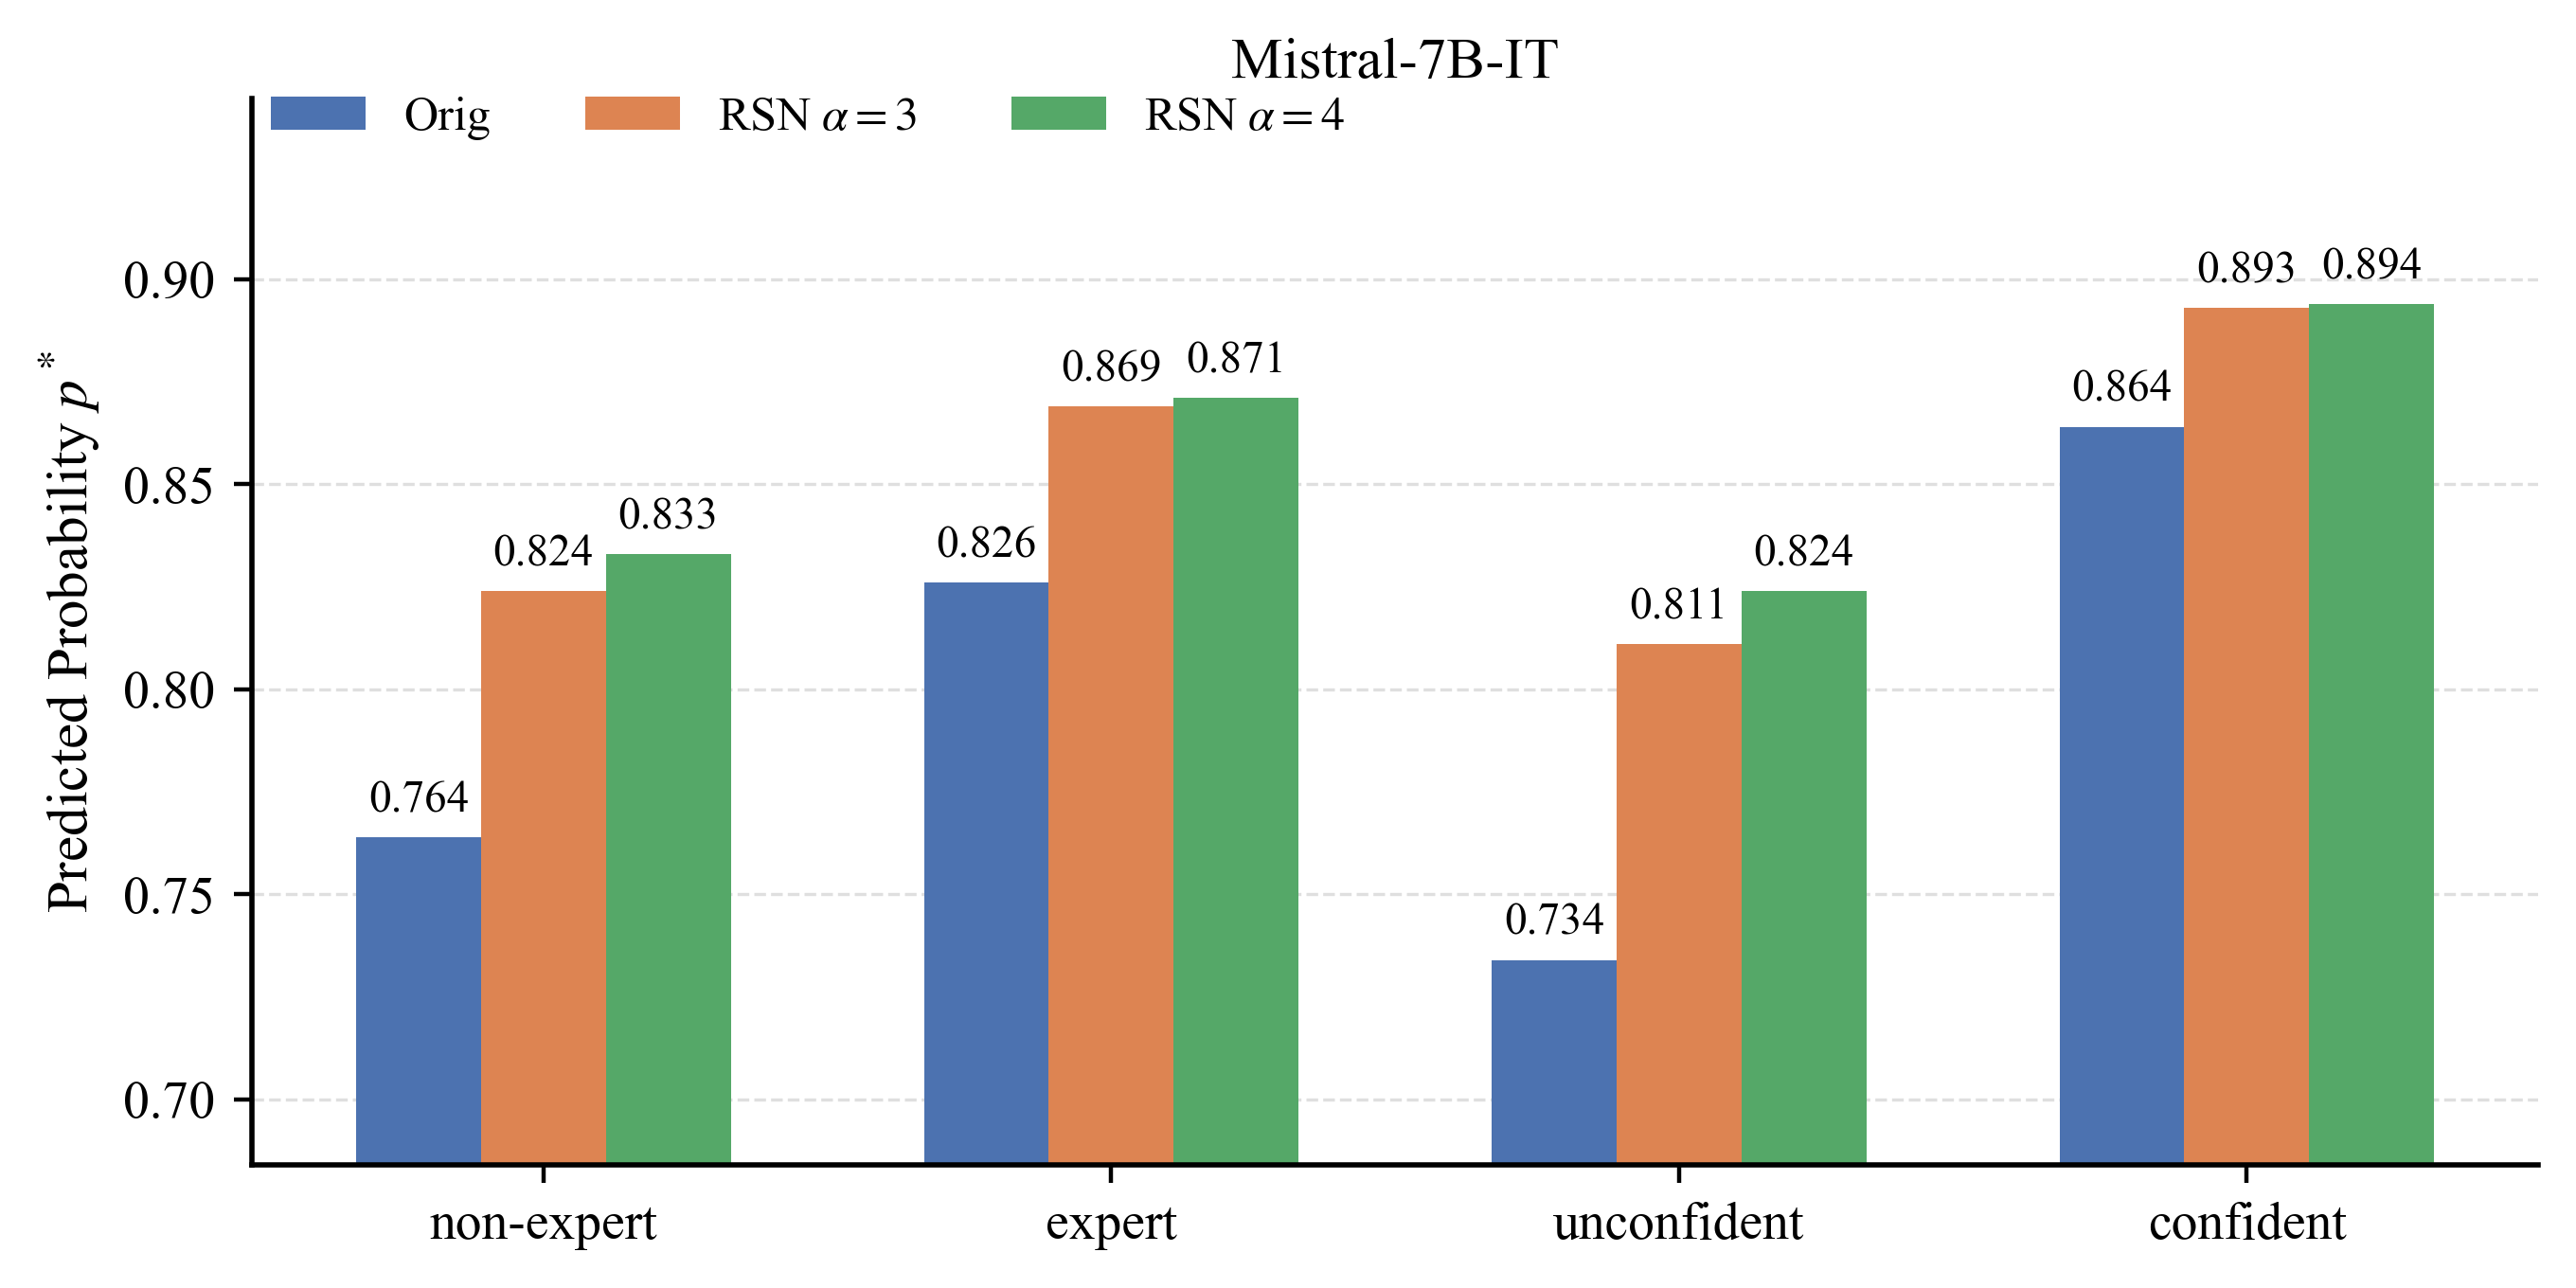
\includegraphics[width=\linewidth]{figure21-mistral.png}
        \caption{\emph{Mistral-7B-IT}}
    \end{subfigure}

    \begin{subfigure}{0.9\linewidth}
        \centering
        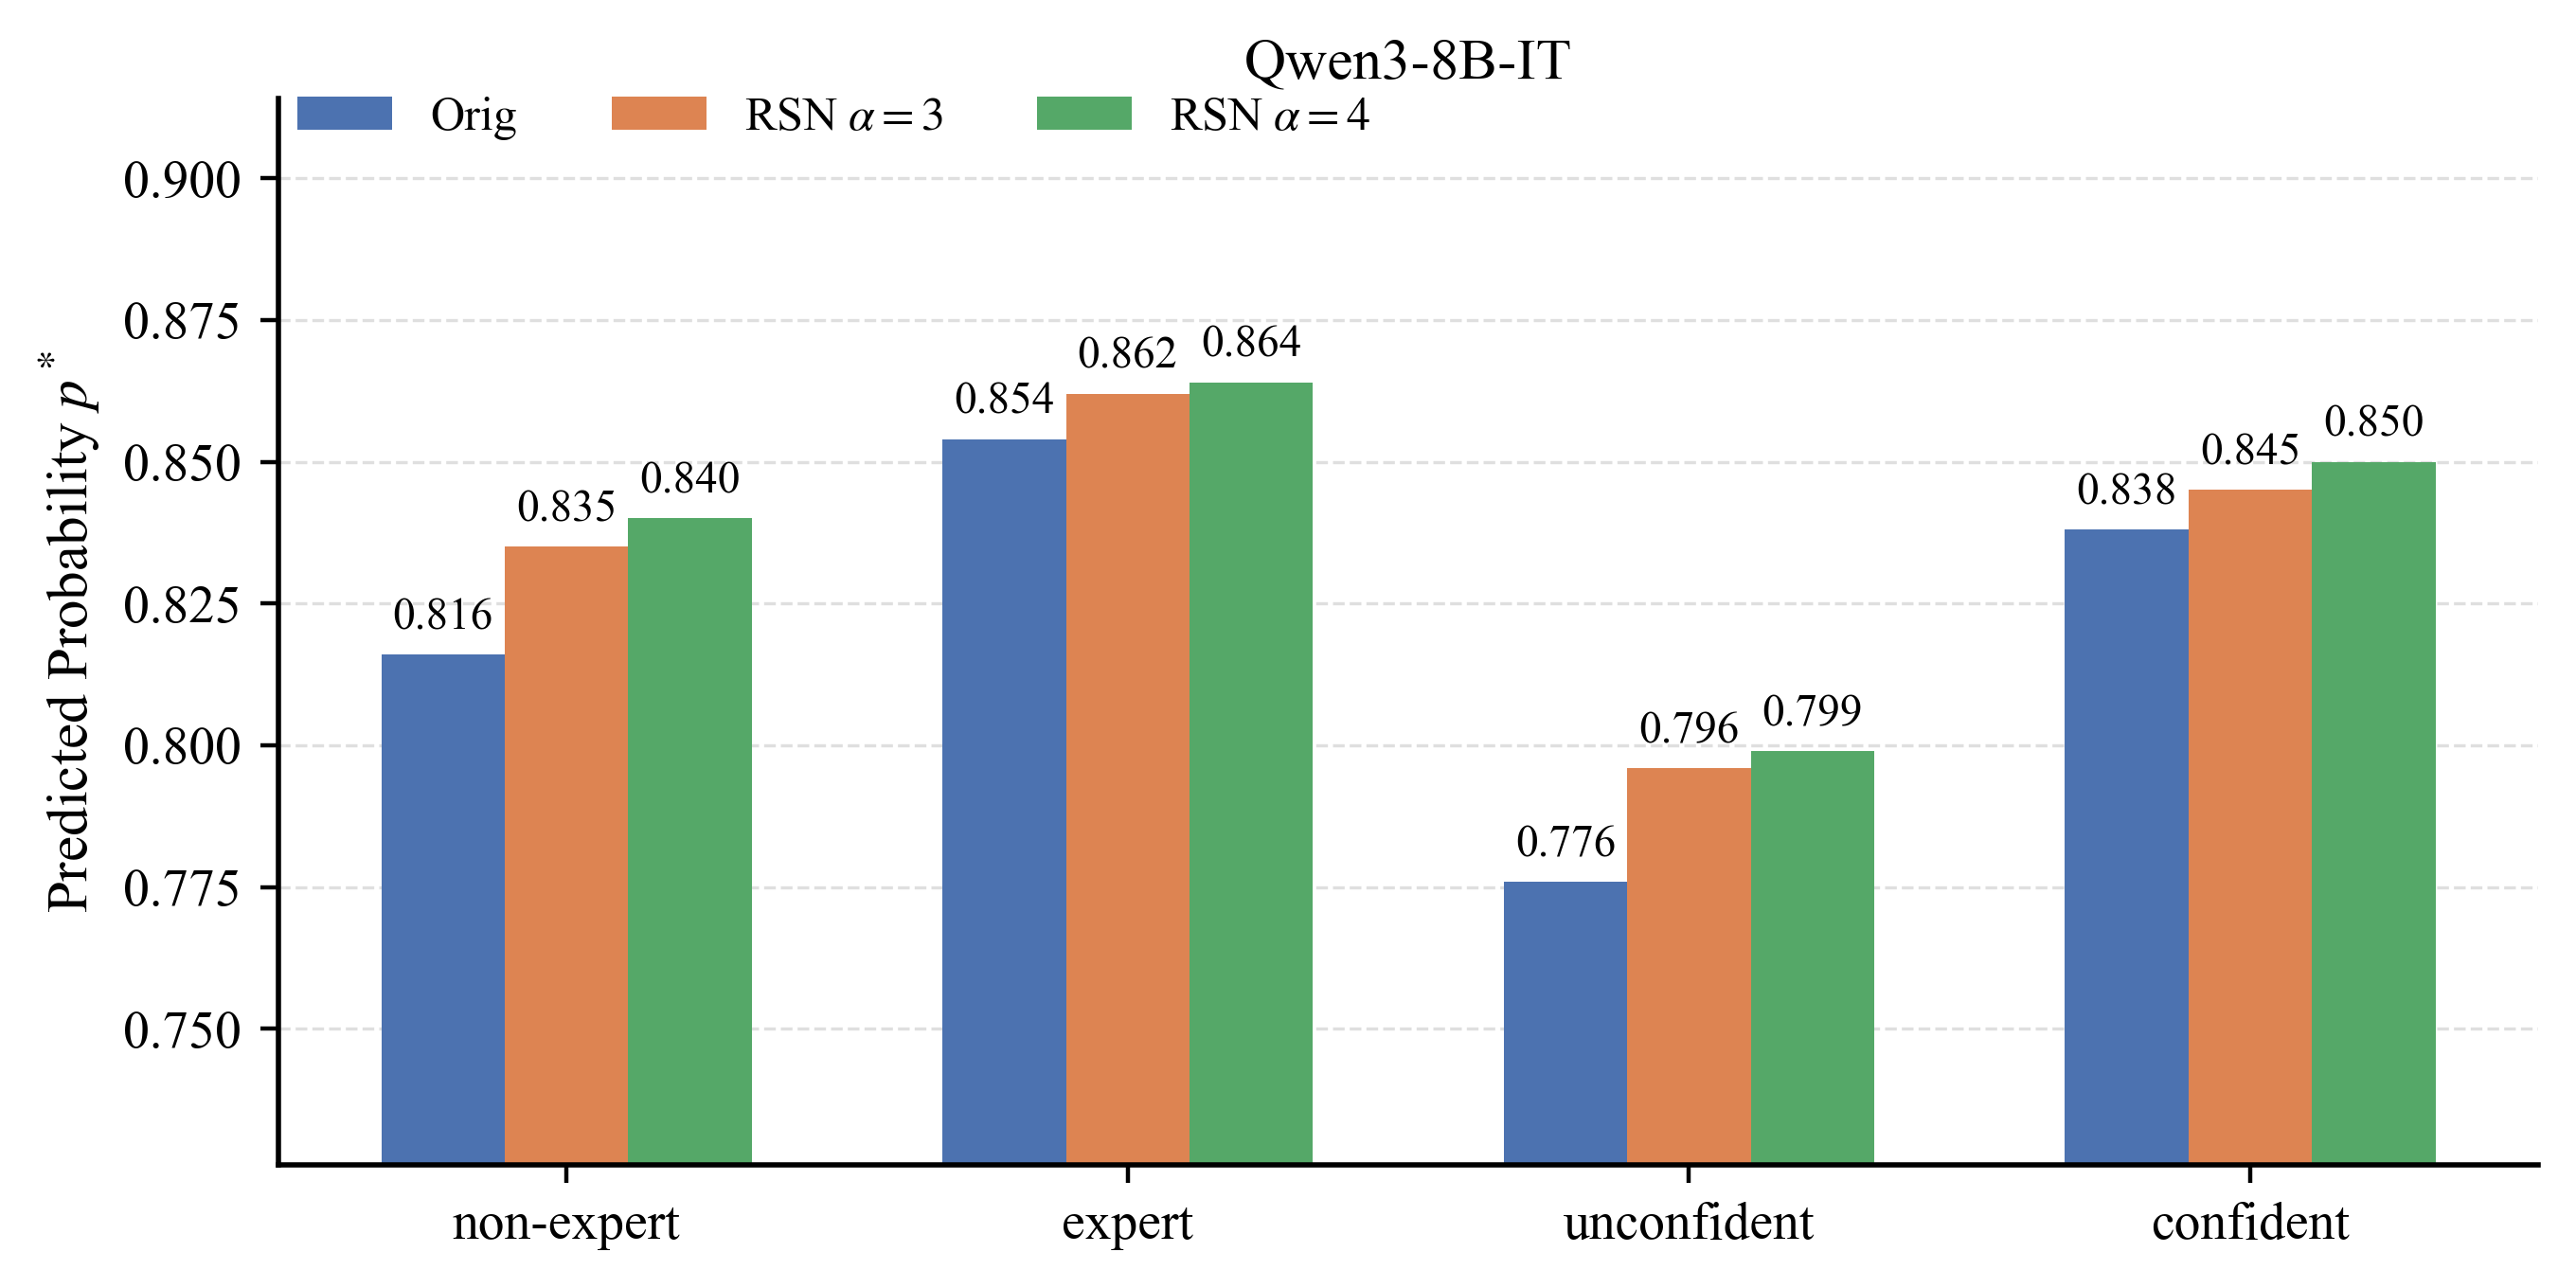
\includegraphics[width=\linewidth]{figure21-qwen3.png}
        \caption{\emph{Qwen3-8B-IT}}
    \end{subfigure}

    \caption{Cross-Model Confidence Enhancement. Predicted probability ($p^*$) under RSN editing. RSN intervention ($\alpha=3, 4$) consistently increases internal confidence across all roles and prompting conditions, replicating the trend shown for Llama3 in Figure~\ref{fig:confidence_shift}.}
    \label{fig:confidence_shift_models}
\end{figure}

\subsection{Cross-Model Consistency of Confidence Enhancement}
\label{app:confidence_shift_models}

To verify that the confidence-enhancing effect of RSN editing is not specific to a single architecture, we replicate the probability analysis from Figure~\ref{fig:confidence_shift} on \emph{Mistral-7B-IT} and \emph{Qwen3-8B-IT}.

Figure~\ref{fig:confidence_shift_models} reports the mean predicted probability ($p^*$) across four prompting conditions (\emph{non-expert}, \emph{expert}, \emph{unconfident}, \emph{confident}) before and after RSN intervention ($\alpha=3, 4$).

Across both models, RSN editing consistently increases $p^*$ relative to the unedited baseline, mirroring the monotonic trend observed in Llama3 (Figure~\ref{fig:confidence_shift}). The largest gains again appear in \emph{non-expert} and \emph{unconfident} settings, confirming that RSNs strengthen internal certainty where the baseline confidence is weakest. Meanwhile, already confident conditions show smaller yet stable improvements, suggesting that RSN scaling saturates once activation approaches a high-certainty regime.

These results demonstrate that the observed confidence amplification is architecture-agnostic: RSN editing provides a consistent, model-general mechanism for increasing internal decisiveness without relying on linguistic cues or fine-tuning.


\begin{figure}[t]
    \centering
    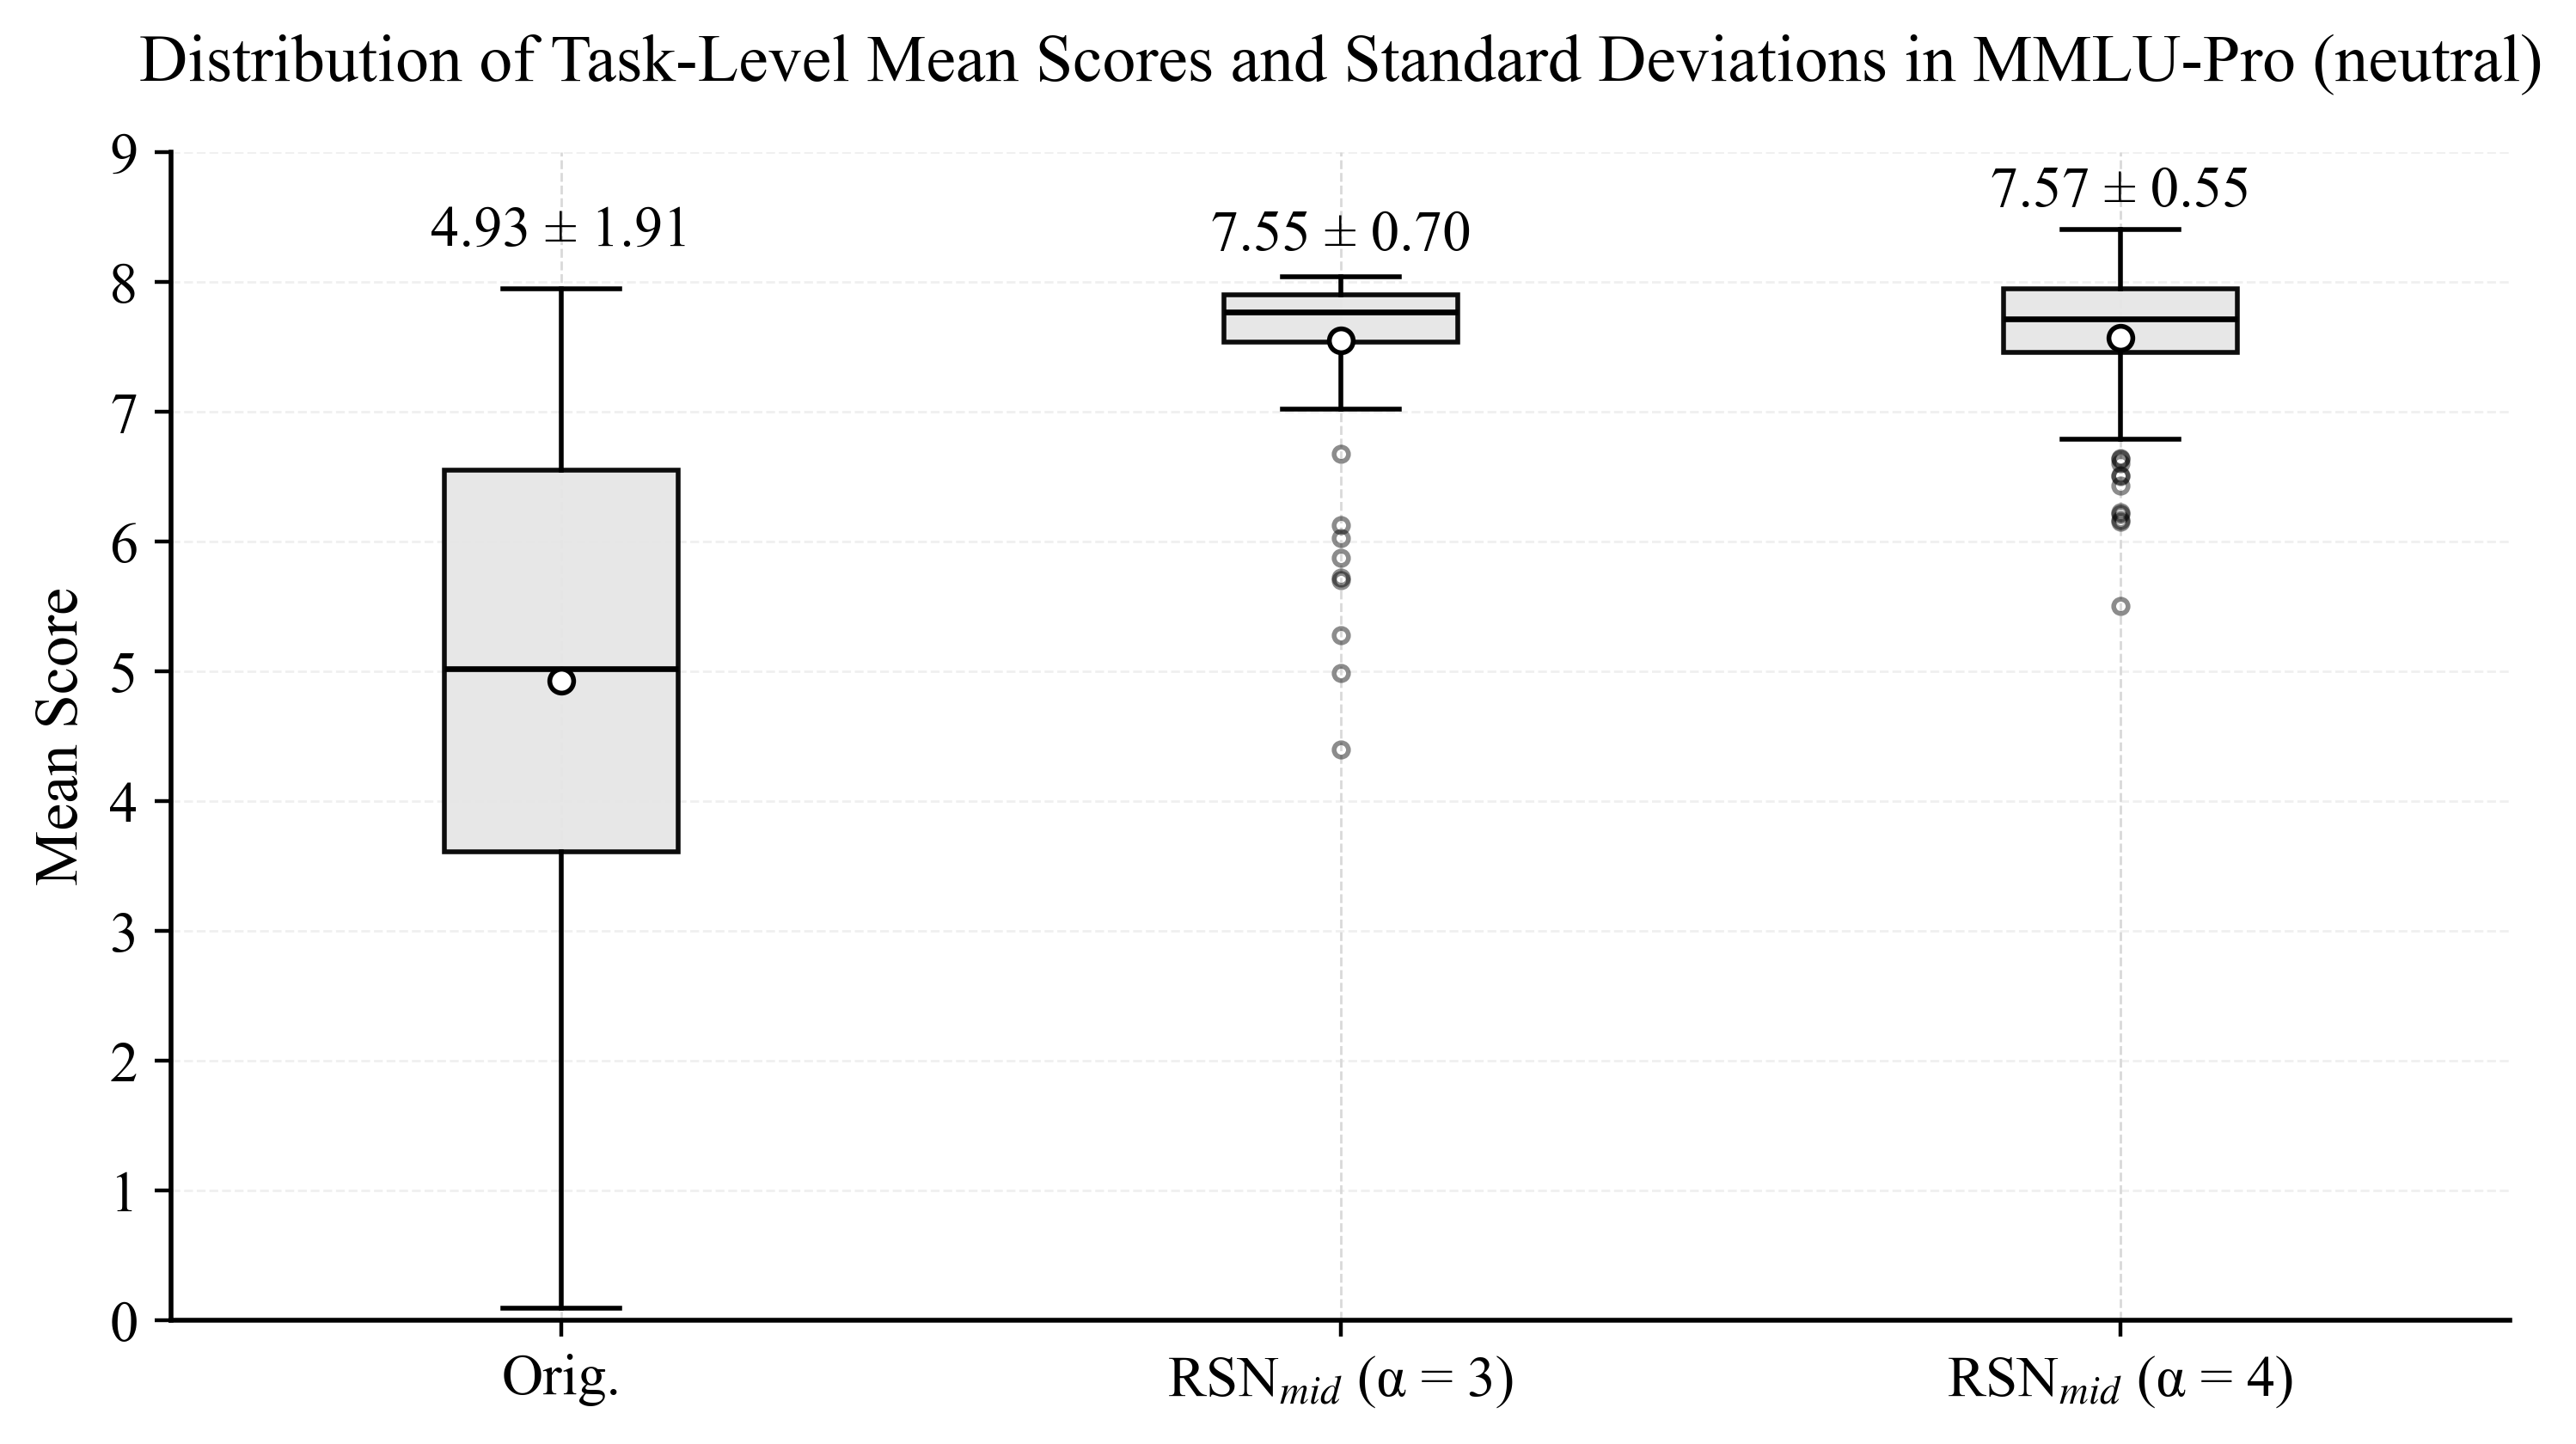
\includegraphics[width=0.95\linewidth]{figure20-box-mmlupro-neutral.png}
    \caption{RSN Effects on Self-Evaluation (Neutral Condition). On \emph{MMLU-Pro} (90 tasks), positive RSN shifts ($\alpha{=}3,4$) raise and compress self-evaluated scores, indicating stabilized internal activations.}
    \label{fig:20-box-mmlupro}
\end{figure}


\subsection{Verbalized Confidence and Entropy Analysis on MMLU-Pro}
\label{app:self-eval-analysis}

To validate whether the shift in internal states (MSP) translates to explicit output, we conduct a comprehensive analysis on \emph{Standard MMLU-Pro}~\cite{wang2024mmlupro}. We focus on two complementary metrics: the distributional shift of explicit confidence scores, and the entropy (stability) of these predictions.

\paragraph{Distributional Shift under RSN.}
We first evaluate the model's ``Reasoning Willingness'' (self-evaluation on a 0--9 scale) under the \textit{Neutral} condition. As shown in Figure~\ref{fig:20-box-mmlupro}, the original model exhibits a broad and highly variable distribution (Mean $\approx 4.9 \pm 1.91$), reflecting unstable certainty when explicit cues are absent. Crucially, RSN injection ($\alpha=3, 4$) transforms this into a compact, high-confidence regime (Mean $\approx 7.6 \pm 0.55$). This contraction of variance and upward shift confirms that RSNs fundamentally restructure the model's internal state to be more decisive.

\begin{figure}[t]
    \centering
    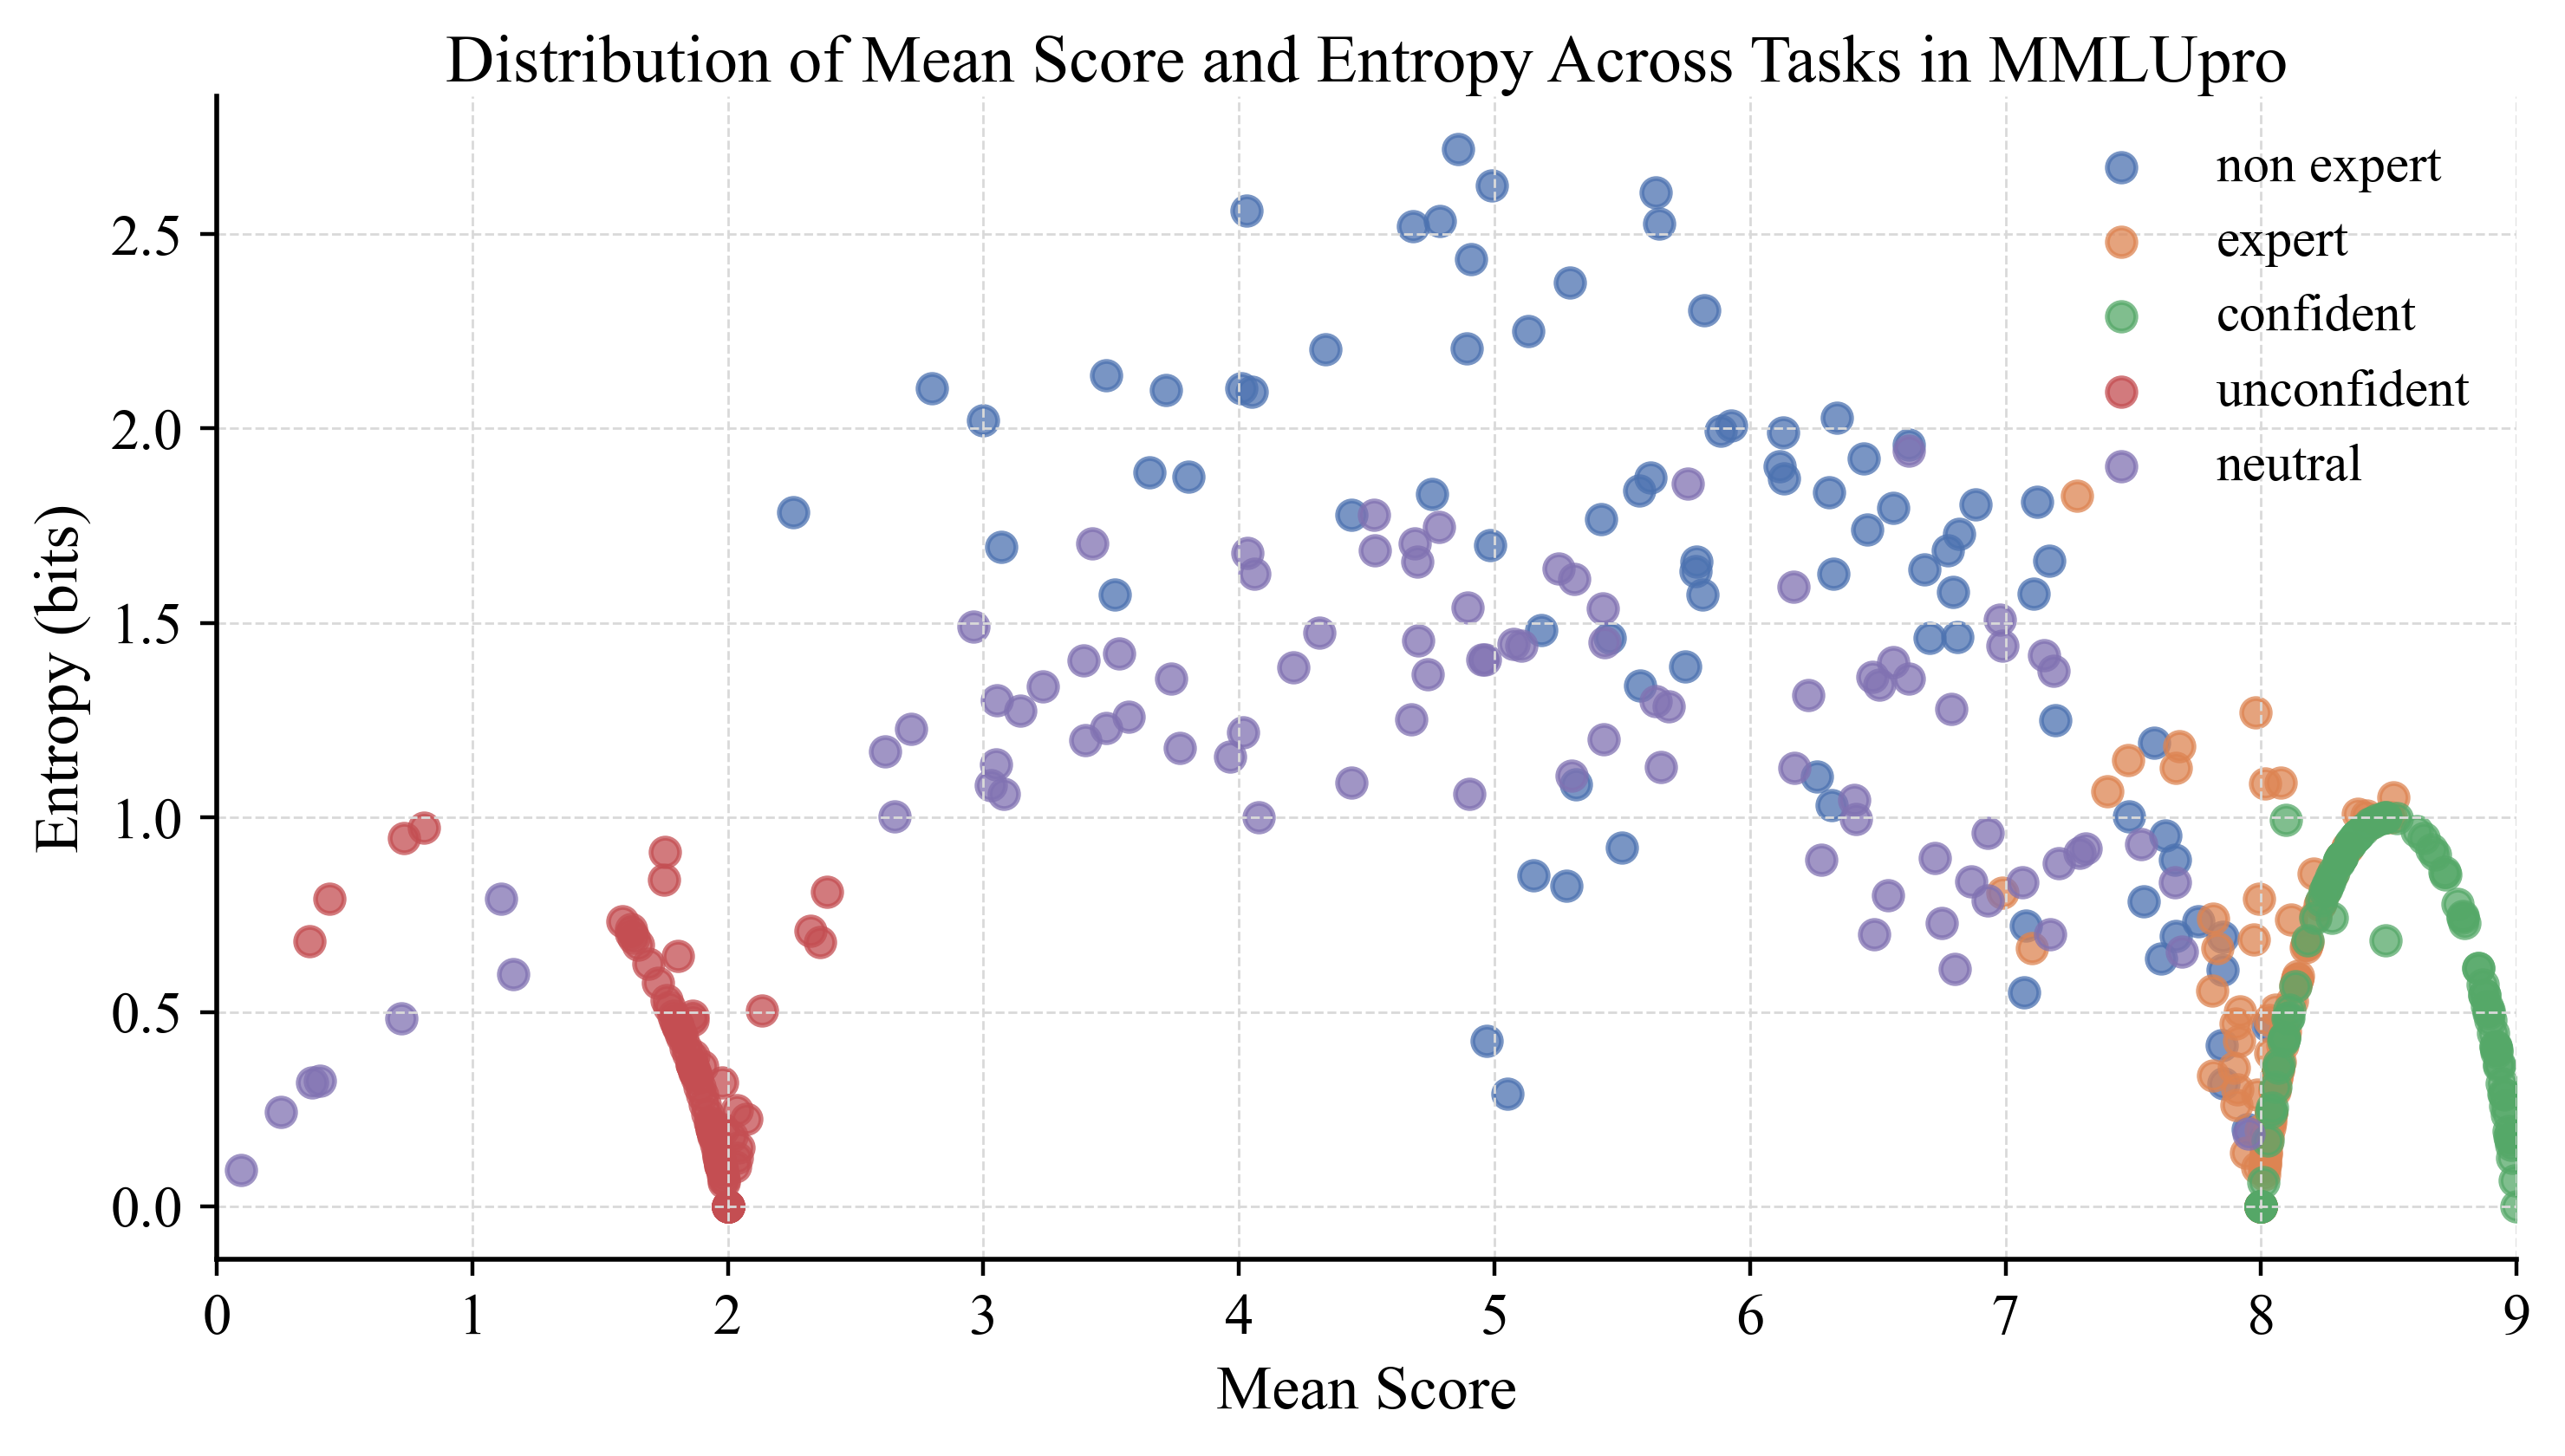
\includegraphics[width=0.95\linewidth]{figure19-entropy-mmlupro.png}
    \caption{Entropy vs. Self-Evaluation Score (MMLU-Pro). Task-level mean scores and entropy values across five prompting conditions. Higher self-confidence systematically correlates with lower entropy (higher stability), confirming that RSN-induced confidence represents a stable, low-entropy state.}
    \label{fig:entropy-mmlupro}
\end{figure}

\paragraph{Entropy and Stability.}
To verify that this increased confidence reflects stable internal states rather than random noise, we analyze the entropy of the self-generated scores. Figure~\ref{fig:entropy-mmlupro} visualizes the relationship between mean scores and entropy across five prompting conditions. A distinct inverse correlation is observed: high-confidence roles (e.g., \emph{confident}, \emph{expert}) occupy low-entropy regions, while low-confidence settings exhibit higher entropy. This confirms that the "confidence" steering not only shifts the mean score but also sharpens the underlying activation distribution.

\subsection{Extended Analysis on Mistral-7B-IT}
\label{app:mistral-analysis}

In the main text, we noted that Mistral-7B-IT exhibits distinct dynamics compared to Llama3 and Qwen3. Here, we provide a comprehensive analysis of this boundary condition, combining performance metrics with mechanistic entropy analysis.

\begin{table*}[t]
\centering
\small
\caption{Mistral-7B-IT Performance in Neutral Settings. Positive steering ($\alpha=4$) fails to improve reasoning, whereas negative steering ($\alpha=-4$) recovers factual accuracy. This highlights that RSNs modulate decision threshold rather than knowledge.}
\label{tab:app-mistral-neutral}
\setlength{\tabcolsep}{5pt}
\renewcommand{\arraystretch}{1.1}
\begin{tabular}{l | ccccc | ccc}
\toprule
\multirow{2}{*}{\textbf{Condition}}
& \multicolumn{5}{c|}{\textbf{Reasoning Benchmarks (Acc \%)}}
& \multicolumn{3}{c}{\textbf{Factuality (Acc \%)}} \\
& MMLU & MMLUPro& GPQA & AR-LSAT & LogiQA
& TQA-MC1 & TQA-MC2 & FACTOR \\
\midrule
\textbf{Orig}
& 59.42 & \textbf{31.67} & 30.34 & 21.47 & 50.00& 46.27 & 57.65 & 66.98 \\
\textbf{+RSN ($\alpha=4$)}
& 58.03 & 28.25 & \textbf{30.65} & 21.23 & 49.81
& 45.90 & 57.04 & 61.97 \\
\textbf{+RSN ($\alpha=-4$)}
& -- & 30.10& 29.26& 20.80& \textbf{51.15}& 45.90 & \textbf{59.73} & \textbf{68.04} \\
\bottomrule
\end{tabular}
\end{table*}

\begin{table*}[t]
\centering
\small
\caption{Detailed linguistic marker counts on GSM8K (300 samples per condition). Llama3 shows clear monotonic trends; Qwen3's higher baseline self-correction reflects its chain-of-thought style.}
\label{tab:gsm8k-markers}
\setlength{\tabcolsep}{5pt}
\renewcommand{\arraystretch}{1.05}
\begin{tabular}{l l ccc}
\toprule
\textbf{Model} & \textbf{Marker Type} & $\alpha=-4$ & \textbf{Neutral} & $\alpha=+4$ \\
\midrule
\multirow{4}{*}{Llama3-8B-IT}
 & Assertive (total)      & 279  & 334  & 427  \\
 & Hedging (total)        & 7    & 13   & 22   \\
 & Self-correction (total)& 3    & 6    & 3    \\
 & \textbf{Confidence Ratio} & 0.91 & 1.08 & \textbf{1.37} \\
\midrule
\multirow{4}{*}{Qwen3-8B-IT}
 & Assertive (total)      & 318  & 297  & 301  \\
 & Hedging (total)        & 722  & 596  & 539  \\
 & Self-correction (total)& 1245 & 1086 & 1042 \\
 & \textbf{Confidence Ratio} & 0.27 & 0.31 & \textbf{0.33} \\
\bottomrule
\end{tabular}
\end{table*}

\subsubsection{Performance Dynamics: The Factuality Trade-off}
As detailed in Table~\ref{tab:app-mistral-neutral}, positive RSN steering ($\alpha=4$) on Mistral does not yield gains on reasoning tasks and significantly impairs factuality. This suggests that blind confidence boosting is ineffective when the base model lacks sufficient latent representations. However, consistent with Llama3, negative steering ($\alpha=-4$) effectively functions as a ``caution filter,'' improving performance on Factuality benchmarks (TruthfulQA-MC2 and FACTOR).

\subsubsection{Mechanism Isolation: The Case of "Unwarranted Certainty"}
To understand \emph{why} accuracy remains flat despite steering, we analyze the model's internal uncertainty distribution via \emph{Constrained Entropy} on MMLU-Pro.

\begin{figure}[t]
\centering
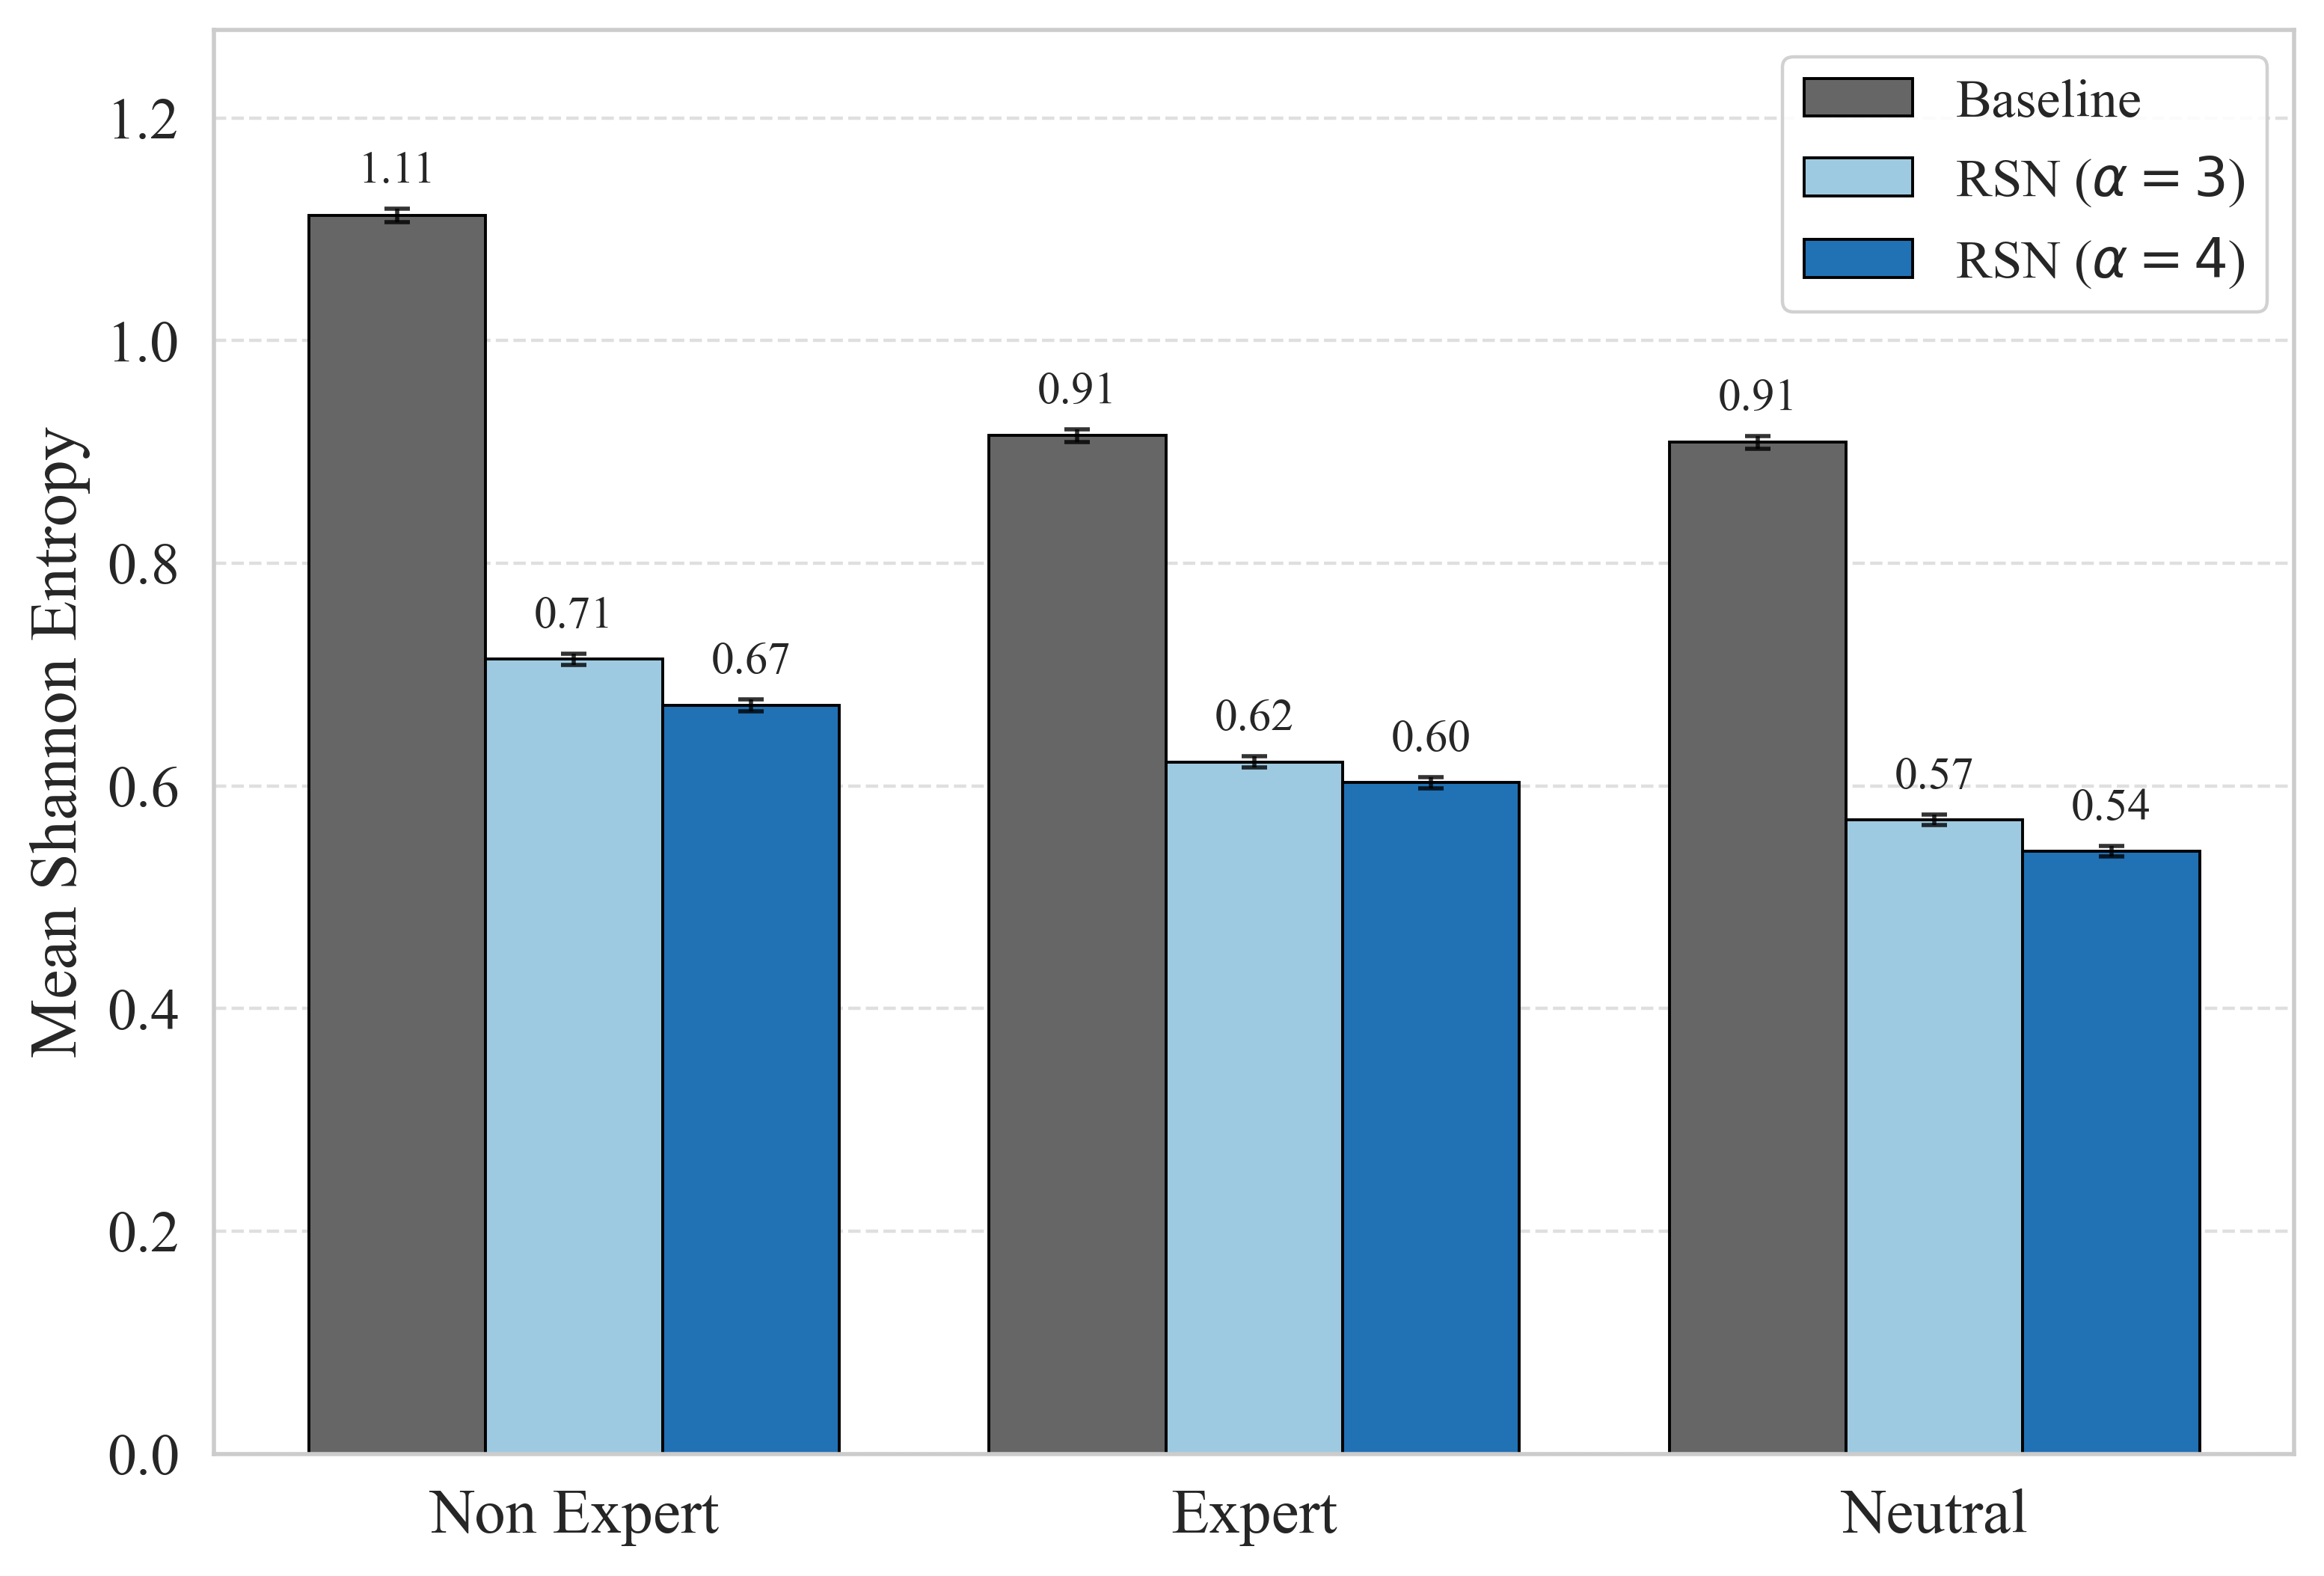
\includegraphics[width=0.95\linewidth]{figure23.png}
\caption{Decoupling Confidence from Capability (Mistral-7B-IT). While accuracy remains flat (Table~\ref{tab:app-mistral-neutral}), RSN editing triggers a drastic drop in Constrained Entropy. This confirms that RSNs amplify certainty independent of correctness.}
\label{fig:mistral-entropy}
\end{figure}

As shown in Figure~\ref{fig:mistral-entropy}, RSN injection triggers a precipitous drop in entropy across all conditions, even though accuracy (Table~\ref{tab:app-mistral-neutral}) does not improve. This decoupling confirms a critical mechanistic insight: RSNs function purely as a \emph{gain control mechanism}. They sharpen the probability distribution to force a decision, but they cannot inject new knowledge. When the underlying knowledge is absent, RSNs simply create "unwarranted certainty," confirming that the mechanism modulates \emph{willingness} rather than \emph{capability}.


\subsection{GSM8K Linguistic Marker Dictionary}
\label{app:gsm8k-markers}

We evaluate linguistic confidence on 300 randomly sampled GSM8K problems per condition (strictly paired across $\alpha \in \{-4, \text{neutral}, +4\}$), with no role prompt. RSN steering is injected solely at the final prompt token during prefill, after which the reasoning chain is generated freely. Detailed per-condition counts and Confidence Ratios for both models are reported in Table~\ref{tab:gsm8k-markers}. The following lexical patterns (exact-match, case-insensitive) define each marker category:

\begin{itemize}[noitemsep]
  \item \textbf{Assertive}: \texttt{the answer is}, \texttt{therefore}, \texttt{we can see / know / conclude}, \texttt{so the answer}, \texttt{simply / simple}, \texttt{just}, \texttt{exact(ly)}, \texttt{hence}
  \item \textbf{Hedging}: \texttt{maybe}, \texttt{I think}, \texttt{might}, \texttt{approximately}, \texttt{I hope it is correct}, \texttt{could be}
  \item \textbf{Self-correction}: \texttt{wait}, \texttt{hmm}, \texttt{actually}, \texttt{I made a mistake}
\end{itemize}


\end{document}